\documentclass[12pt]{report} % Times New Roman, 12pt
\pdfminorversion=7 % Included figure PDFs are PDF 1.7; avoids pdfTeX inclusion warnings
%\usepackage{gscale_thesis_singlespace} % Single spaced thesis
\usepackage{gscale_thesis_doublespace} % Double spaced thesis
\usepackage{fancyheadings} % Header and footer styling
\usepackage[round]{natbib} % Bibliography formatting
\usepackage{setspace} % Allows double spacing but skips headers/footers
\setcounter{tocdepth}{1} % Limits the TOC to chapter and section names

% Additional packages
\usepackage{graphicx} % Allows the inclusion of figures
\usepackage{subcaption} % Allows captions to be added to subfigures
\usepackage[justification=centering]{caption} % Centres caption text
\usepackage{array} % Used for table formatting
\newcolumntype{P}[1]{>{\raggedright\let\newline\\\arraybackslash\hspace{0pt}}m{#1}}
\usepackage{booktabs} % Fancy-style tables
\usepackage{longtable} % Allows for tables that are more than one page long
\usepackage{float} % Better figure placement control
\usepackage{tikz} % Vector diagrams (e.g. candidate-selection flow)
\usetikzlibrary{shapes.geometric, arrows.meta, positioning, fit}
\usepackage{enumerate} % Numbered lists
\usepackage[shortlabels]{enumitem} % For controlling enumerate labels
\usepackage[shortcuts]{extdash} % Allows manual hyphenation of hypenated words
\usepackage{amsmath} % Non-standard math symbols
\usepackage{amsfonts} % Extended fonts for mathematics

\usepackage[hidelinks]{hyperref} % Linking to LaTeX labels and external URLs

% Supplementary project materials (mention-count ranking spreadsheet, source
% catalogue, and measurement data) hosted in the smiths/AIMSS repository.
\newcommand{\suppurl}{\url{https://github.com/smiths/AIMSS/tree/master/StateOfPractice/DomainMeasurements/MPS-Ryan}}

\numberwithin{equation}{section} % Numbers equations based on their section



% ********************************
\begin{document}
\title{A State-of-the-Practice Study of Robotics Software for Motion Planning and Simulation}
\halftitle{Robotics Software State of the Practice} % 60 Characters Max. Including Spaces

\author{Ziyang Fang}
\shortauthor{Z. Fang} % Used for page header

\dept{Department of Computing and Software}
\field{Software Engineering} % What field your thesis is in (e.g. Software Engineering)

\prevdegreeone{B.Eng. (Mechanical Design, Manufacturing and Automation),\\ Fuzhou University, School of Mechanical Engineering, China}
\prevdegreetwo{B.Eng.} % Just your degree's field

\submitdate{June 2026} % TODO: confirm the actual submission month before final submission
\copyrightyear{2026} % Year you are submitting this, usually your graduation
%year

\doctype{Report} % ``Report'' or ``Thesis'' or whatever you need
\degree{Master of Engineering} % The degree you get when you submit this
\degreeabbrv{M.Eng.}
\principaladviser{Spencer Smith} % Supervisor. Dr. Matthew Giamou is the domain expert (see Declaration/Acknowledgements), not a co-supervisor -- confirm if this is wrong.
 % LaTeX variables for preface pages/headers
    
\beforepreface % Half title page, title page, declaration page   
  \prefacesection{Lay Abstract}

Robots are usually tested in software simulations before they are trusted in
the real world. The quality of the software that plans robot motions and
simulates robot behaviour therefore matters to everyone who builds or studies
robots. This report examines 28 widely used open-source packages for robot
motion planning and simulation and grades each one on qualities such as how
easy it is to install, how well it is documented, and how actively it is
maintained, using only publicly visible evidence. The study finds that this
software is generally in good shape: installation support and documentation
are strong, although written design information is often missing. The report
also shows that a package's popularity does not always match its measured
quality.
 % Lay Abstract
  \prefacesection{Abstract}

% TODO: revisit after the developer-interview component is complete (RQ6--RQ9).

Software for motion planning and simulation (MPS) supports the design, testing,
and deployment of robotic systems. Because experiments and applications depend
on this software behaving correctly, its engineering quality matters beyond any
single project. This report assesses the state of the practice for MPS software
by adapting the research-software assessment methodology of Smith et al.
Candidate packages were gathered from academic surveys, community-curated
lists, and auxiliary LLM-assisted discovery; after consolidation of 295 unique
candidate names and filtering by open-source availability, repository-based
measurability, and maintenance activity, 28 packages were selected, spanning
full simulators, physics and dynamics engines, motion planning libraries, and
middleware. Each package was measured in May 2026 against a standard template
covering installability, correctness and verifiability, surface reliability,
surface robustness, surface usability, maintainability, reusability, surface
understandability, and visibility and transparency, together with repository
metrics. A commonality analysis describes the selected packages as a software
family.

The measured packages show strong practical infrastructure: all 28 provide
installation instructions, installation automation, tutorials, user manuals,
and API documentation, and only two installations broke during measurement.
Weaknesses concentrate in formal artifacts: only one package documents expected
user characteristics, and half do not identify a coding standard. Measured
quality and community popularity diverge for several packages, so popularity
indicators such as GitHub stars are not reliable proxies for engineering
quality. Compared with prior studies of the state of the practice for medical imaging
and Lattice Boltzmann method software, MPS software is at least as well
equipped in repository artifacts and development tooling. A developer-interview
component has been designed to investigate pain points and practices; its
execution is left for future work.
 % Abstract
  %\include{dedic} % Dedication (optional) -- re-enable after personalizing dedic.tex
  \prefacesection{Acknowledgements}

% TODO: personalize before submission.

I would like to thank my supervisor, Dr.~Spencer Smith, for his guidance and
feedback throughout this work. I would also like to thank Dr.~Matthew Giamou,
who served as the domain expert for this study, for reviewing the candidate
software list and for his advice on the scope, inclusion, and exclusion
decisions.
 % Acknowledgements
  \referencepages % Table of Contents, List of Figures, List of Tables
  \prefacesection{Notation, Definitions, and Abbreviations}

\section*{Notation}
\begin{description}[font=\rmfamily\bfseries, leftmargin=3cm, style=nextline]
	\item[$s_i$] Impression score (1--10) of package $i$ on a given quality (Analytic Hierarchy Process)
	\item[$a_{ij}$] Pairwise comparison value between packages $i$ and $j$ on a given quality (Analytic Hierarchy Process)
	\item[$w_i$] Priority of package $i$ on a given quality (Analytic Hierarchy Process)
	\item[$c_k$] Weight of quality $k$ (Analytic Hierarchy Process)
	\item[$p_i$] Overall priority of package $i$ across the nine qualities (Analytic Hierarchy Process)
	\item[$n$] Number of packages, i.e.\ the dimension of a pairwise-comparison matrix (Analytic Hierarchy Process)
\end{description}

\section*{Definitions}
\begin{description}[font=\rmfamily\bfseries, leftmargin=3cm, style=nextline]
	\item[Alive package] In this report, a package is considered alive if it has received any commit or release in the 18 months preceding the measurement date.
	\item[Software family] A set of programs whose common properties are extensive enough that studying them collectively is advantageous before analysing individual members~\citep{Parnas1976}.
	\item[State-of-the-Practice study] An assessment of the artifacts, tools, processes, and quality of existing software in a chosen domain, in contrast to a study that designs or implements new software.
	\item[Surface measure] An assessment based on shallow but systematic checks performed within a limited time budget rather than on exhaustive experimental evaluation.
\end{description}

\section*{Abbreviations}
\begin{description}[font=\rmfamily\bfseries, leftmargin=3cm, style=nextline]
	\item[AHP] Analytic Hierarchy Process
	\item[AIST] National Institute of Advanced Industrial Science and Technology (Japan)
	\item[API] Application Programming Interface
	\item[CI] Continuous Integration
	\item[CI/CD] Continuous Integration and Continuous Delivery
	\item[CVC] Computer Vision Center (Barcelona)
	\item[DART] Dynamic Animation and Robotics Toolkit
	\item[DDS] Data Distribution Service
	\item[GIS] Geographic Information Systems
	\item[IIT] Istituto Italiano di Tecnologia (Italian Institute of Technology)
	\item[LBM] Lattice Boltzmann Method
	\item[LLM] Large Language Model
	\item[MI] Medical Imaging
	\item[MREB] McMaster Research Ethics Board
	\item[MJCF] MuJoCo XML configuration format
	\item[MPS] Motion Planning and Simulation
	\item[OMG] Object Management Group
	\item[OMPL] Open Motion Planning Library
	\item[OSS] Open Source Software
	\item[RL] Reinforcement Learning
	\item[ROS] Robot Operating System
	\item[SCC] Sloc, Cloc and Code (the source-code line-counting tool used for the repository measurements)
	\item[SDF] Simulation Description Format
	\item[SDK] Software Development Kit
	\item[SLAM] Simultaneous Localization and Mapping
	\item[SOFA] Simulation Open Framework Architecture
	\item[SOP] State-of-the-Practice
	\item[TRI] Toyota Research Institute
	\item[URDF] Unified Robot Description Format
	\item[YARP] Yet Another Robot Platform
\end{description}

  \academicstatement{academicachievementdeclaration}
\afterpreface
  
  \chapter{Introduction}
\label{ch:introduction}

Robotics software for motion planning and simulation (MPS) enables researchers and engineers to model robot kinematics and dynamics, simulate sensor data, plan collision-free trajectories, and test control strategies before deploying to physical hardware. An application of MPS software is shown in Figure~\ref{fig:motion-planning-example}.

\begin{figure}[H]
    \centering
    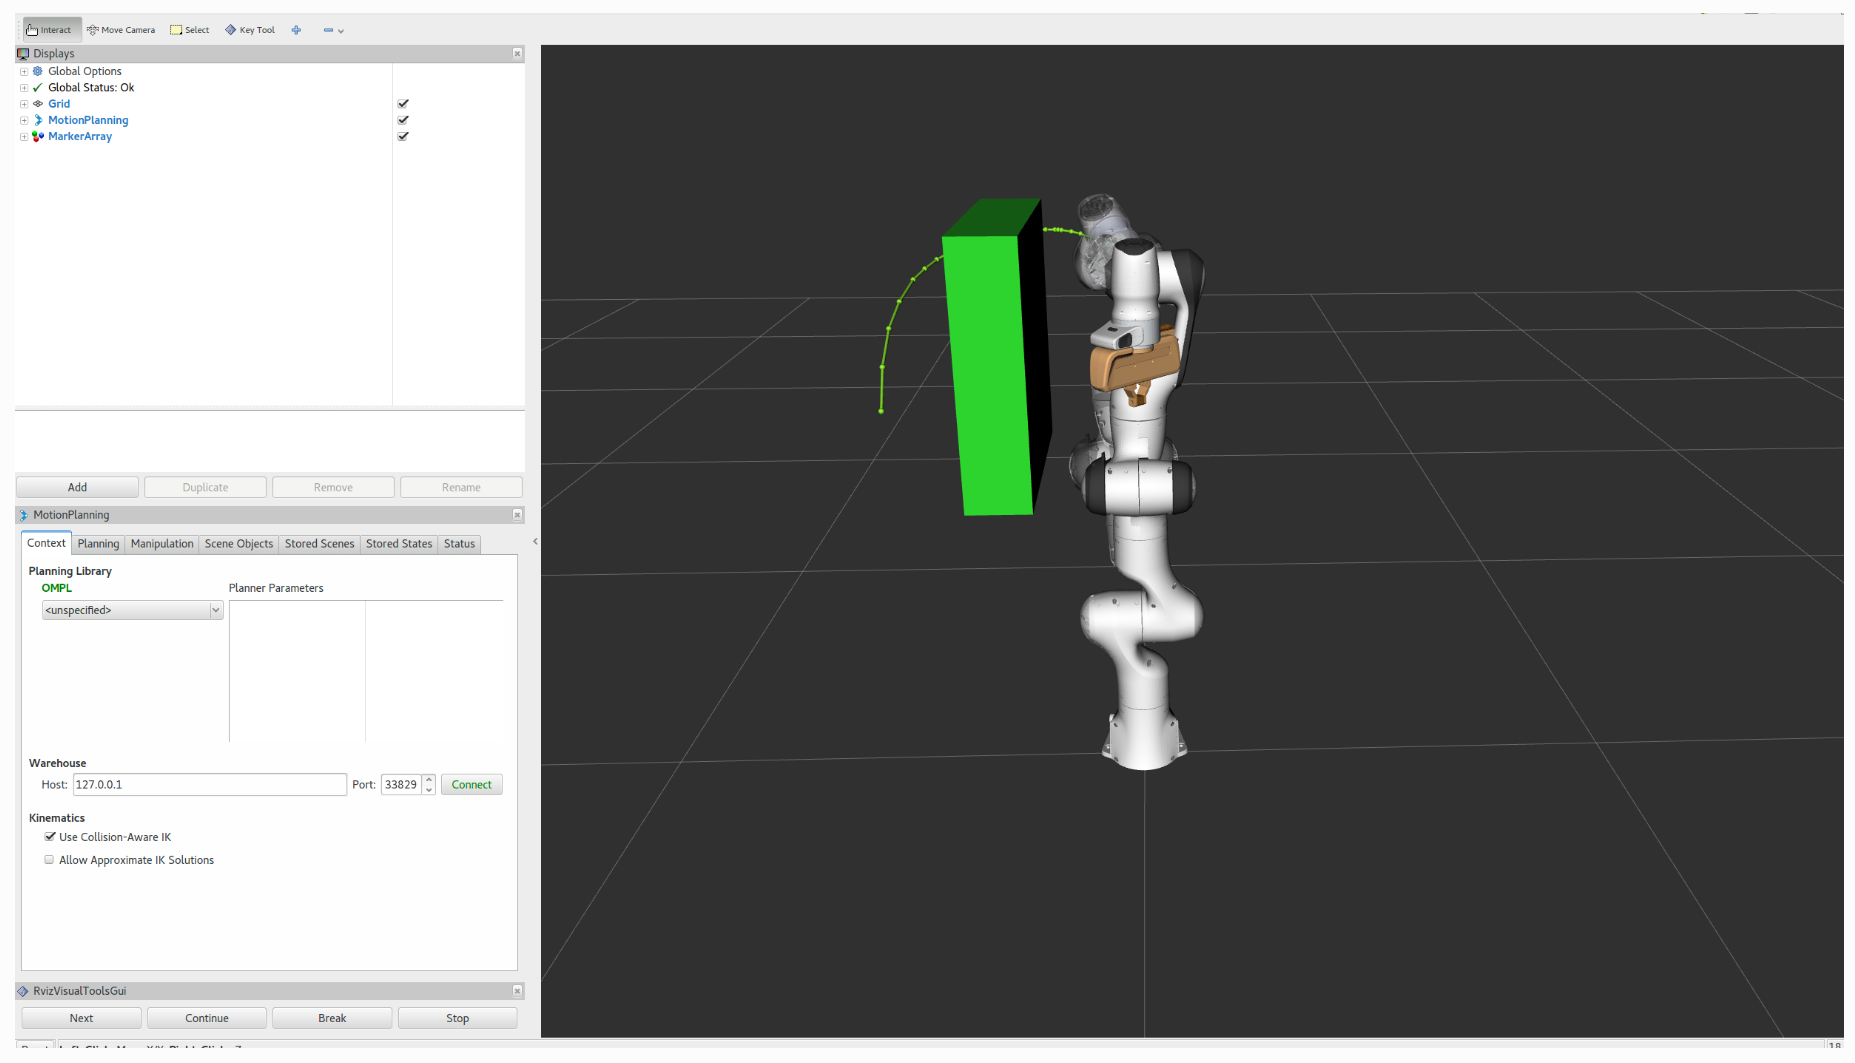
\includegraphics[width=0.95\textwidth]{figures/chapter1-motion-planning}
    \caption{An illustrative path planning task: a manipulator computing a collision-free path around an obstacle.}
    \label{fig:motion-planning-example}
\end{figure}

In practice, this software is central to experimental reproducibility and to the transition from simulation to physical deployment, so qualities such as correctness, reliability, and long-term sustainability have direct consequences for both research and operational outcomes. A simulator that produces incorrect trajectories, or a planner that crashes under realistic inputs, can compromise experimental results.

Software engineers have developed methods and tools for improving software quality: version control, automated testing, and continuous integration are standard practice in professional contexts. However, a gap exists between these practices and what researchers actually do when developing scientific software. Scientists and engineers working on research software tend to learn software engineering skills informally, picking them up from colleagues or through trial and error rather than through formal training~\citep{Hannay2009}. \citet{Hannay2009} observe that many scientists show indifference to standard software engineering concepts, and \citet{Prabhu2011} report that more than half of the scientists they surveyed did not use a debugger. Because much of the software studied in this report originates in research settings, these concerns apply directly to the MPS domain.

Previous studies of the state of the practice have investigated this gap across several scientific software domains, most recently medical imaging~\citep{Smith2024MI} and Lattice Boltzmann method software~\citep{Smith2024LBM}; Section~\ref{sec:state-of-practice-background} reviews these studies. This report adapts the same methodology~\citep{Smith2021} to MPS software. The aim is to understand how MPS software holds up against established software engineering practices and how it compares with other research software domains. The report ranks the selected packages according to the defined quality attributes; these rankings describe the current state of the practice in software development, rather than serving as recommendations for any particular software package.

The remainder of this chapter states the research questions (Section~\ref{sec:research-questions}), defines the scope (Section~\ref{sec:introduction-scope}), overviews the methodology (Section~\ref{sec:methodology-overview}), lists the contributions (Section~\ref{sec:contributions}), and outlines the remaining chapters (Section~\ref{sec:organization}).

\section{Research Questions}
\label{sec:research-questions}

The following research questions guide this report.

\begin{enumerate}[RQ1.]
    \item What software packages are candidates for the study of the state of the practice for MPS software?
    \item What is the ranking of the candidate packages from RQ1 with respect to the software qualities of installability, correctness and verifiability, surface reliability, surface robustness, surface usability, maintainability, reusability, surface understandability, and visibility and transparency?
    \item How do MPS projects compare to other research software domains with respect to the artifacts present in their repositories?
    \item How do MPS projects compare to other research software domains with respect to the use of tools?
    \item How do MPS projects compare to other research software domains with respect to the principles, processes, and methodologies used?
    \item What are the pain points for developers working on MPS software projects?
    \item How do the pain points for MPS developers compare to the pain points for developers in other research software domains?
    \item For MPS developers, what specific best practices address the pain points identified in RQ6 and the software qualities mentioned in RQ2?
    \item What research software development practices, beyond those already used by MPS developers, address the pain points identified in RQ6?
\end{enumerate}

RQ1--RQ5 are answered from public artifacts, while RQ6--RQ9 depend on the developer-interview component.

\section{Scope}
\label{sec:introduction-scope}

This report covers MPS software: robotics packages for motion planning, dynamics, physics, simulation, and supporting middleware. To be included, a package must expose sufficient public evidence, such as a source repository, documentation, issue tracker, releases, or project metadata, to support consistent repository-based measurement. Tools whose core components are proprietary or otherwise closed therefore fall outside the measured set even if they are widely used in robotics practice. Chapter~\ref{ch:methodology} states the full inclusion and exclusion criteria and gives the rationale for individual tools that were considered and removed.

The selected packages play different roles within shared MPS workflows; Chapter~\ref{ch:selected-software-commonality} explains those roles before the measurement results are interpreted.

\section{Overview of the Methodology}
\label{sec:methodology-overview}

This report follows the methodology of \citet{Smith2021} (hereafter the Domain~X methodology): it defines the MPS domain, identifies candidate packages from academic, community-curated, and auxiliary LLM-assisted sources, filters them to a measurable set, measures and ranks the selected packages from their public artifacts, analyzes them as a software family, compares the findings with prior domain studies, and prepares the developer-interview component. Chapter~\ref{ch:methodology} details each step. The scope and exclusions were reviewed with a domain expert to reduce the risk of misrepresenting the MPS domain.

\section{Contributions}
\label{sec:contributions}

This report makes the following contributions:

\begin{enumerate}
    \item A scoped study of the state of the practice for MPS software, applying the methodology of \citet{Smith2021} to a new domain.
    \item A transparent candidate discovery and selection process that combines academic sources, community-curated lists, and auxiliary LLM-assisted discovery, with explicit discussion of the role and limitations of each source type.
    \item A public-artifact measurement dataset for 28 selected software packages, covering repository evidence, documentation, releases, issue trackers, testing and continuous-integration evidence, and project metadata, organized across the nine quality categories defined in the measurement template of \citet{Smith2021}.
    \item A commonality analysis identifying shared capabilities, variability points, and parameters of variation across the selected packages.
    \item A comparison of MPS software with findings from prior studies of the state of the practice in other research software domains~\citep{Smith2024LBM,Smith2024MI,Smith2018Seismology}.
\end{enumerate}

These contributions are descriptive and methodological.

\section{Organization}
\label{sec:organization}

The remainder of this report is organized as follows. The research questions are not confined to a single chapter; they are answered throughout the body, and each chapter notes the research questions it addresses to maintain traceability back to Section~\ref{sec:research-questions}.

\begin{itemize}
    \item \textbf{Chapter~\ref{ch:background}} provides background on the MPS domain, prior studies of the state of the practice, the nine quality attributes, commonality analysis, and the Analytic Hierarchy Process.
    \item \textbf{Chapter~\ref{ch:methodology}} describes the methodology, from domain selection and candidate discovery to measurement, commonality analysis, and the interview component.
    \item \textbf{Chapter~\ref{ch:selected-software-commonality}} presents the 28 selected packages as a software family and reports the commonality analysis.
    \item \textbf{Chapter~\ref{ch:measurement-results}} reports the measurement results, the quality-based rankings, and their comparison with community-facing indicators.
    \item \textbf{Chapter~\ref{ch:comparison-research-software}} compares MPS software with prior studies in other research software domains.
    \item \textbf{Chapter~\ref{ch:developer-interviews}} sets out the developer-interview component for RQ6--RQ9.
    \item \textbf{Chapter~\ref{ch:recommendations}} gives recommendations for future MPS software practice.
    \item \textbf{Chapter~\ref{ch:threats-to-validity}} discusses threats to validity.
    \item \textbf{Chapter~\ref{ch:conclusions}} summarizes the study, answers the research questions, and identifies directions for future work.
\end{itemize}

        \setcounter{figure}{0}
        \setcounter{equation}{0}
        \setcounter{table}{0}

  \chapter{Background}
\label{ch:background}

This chapter sets out the concepts the rest of the report relies on: the MPS domain, the software licensing categories, state-of-the-practice methodology, the nine quality attributes, commonality analysis, the Analytic Hierarchy Process, and the role of repository-based measurement.

\section{Robotics Software for Motion Planning and Simulation}
\label{sec:robotics-software-background}

MPS software supports the design, testing, evaluation, and deployment of robotic systems. Motion planning software generates feasible robot motions under constraints such as geometry, kinematics, dynamics, collisions, and task requirements~\citep{lavalle2006planning}. Simulation software provides virtual environments for representing robots, sensors, actuators, controllers, and physical interactions before, or alongside, work with physical hardware~\citep{collins2021simulators}.

The MPS domain in this report is defined to span more than a single class of software, so that the study includes enough packages to support a meaningful comparison. It covers full simulation environments, physics and dynamics engines, motion planning libraries, manipulation frameworks, and middleware. These classes of software are not interchangeable, but they are unified because they appear together in the same workflow: a simulator may call a physics engine for contact and dynamics, a planning stack may sit on top of a collision-checking library and communicate through middleware, and middleware may call planning, control, perception, and simulation. Figure~\ref{fig:mps-software-stack} sketches these relationships among the four software roles; the report is explicit throughout about which role each package plays.

\begin{figure}[htbp]
\centering
% Figure palette: the two structural rails (middleware, physics) share one
% neutral slate; the two subject roles (planning, simulation) each carry one
% accent. Three colours total, each with a matching deeper border.
\definecolor{mpsSlateFill}{HTML}{EDEEF1}
\definecolor{mpsSlateLine}{HTML}{5E6675}
\definecolor{mpsSlateText}{HTML}{394150}
\definecolor{mpsTealFill}{HTML}{E0F1EC}
\definecolor{mpsTealLine}{HTML}{0F8E78}
\definecolor{mpsTealText}{HTML}{0A5446}
\definecolor{mpsBlueFill}{HTML}{E6EEFA}
\definecolor{mpsBlueLine}{HTML}{2C6FCE}
\definecolor{mpsBlueText}{HTML}{1A4A8F}
\definecolor{mpsArrow}{HTML}{7A828C}
\begin{tikzpicture}[
  font=\small,
  comp/.style={draw, rounded corners, align=center, inner sep=5pt, minimum height=1.15cm, line width=0.8pt},
  mw/.style={comp, fill=mpsSlateFill, draw=mpsSlateLine, text=mpsSlateText, text width=9cm},
  plan/.style={comp, fill=mpsTealFill, draw=mpsTealLine, text=mpsTealText, text width=4cm},
  sim/.style={comp, fill=mpsBlueFill, draw=mpsBlueLine, text=mpsBlueText, text width=4cm},
  phys/.style={comp, fill=mpsSlateFill, draw=mpsSlateLine, text=mpsSlateText, text width=9cm},
  bus/.style={{Latex[length=2mm]}-{Latex[length=2mm]}, thick, draw=mpsArrow},
  uses/.style={-{Latex[length=2.6mm]}, thick, draw=mpsArrow},
]
\node[mw] (mw) at (2.5,0) {\textbf{Middleware} \footnotesize(ROS~2, YARP)\\[1pt]\footnotesize communication, hardware abstraction, system integration};
\node[plan] (plan) at (0,-2.25) {\textbf{Motion planning \&}\\\textbf{manipulation}\\[1pt]\footnotesize OMPL, MoveIt!};
\node[sim] (sim) at (5,-2.25) {\textbf{Simulation}\\\textbf{environments}\\[1pt]\footnotesize Gazebo, Webots, CoppeliaSim, CARLA};
\node[phys] (phys) at (2.5,-5.15) {\textbf{Physics \& dynamics engines}\\[1pt]\footnotesize Bullet, MuJoCo, ODE, DART};
\draw[bus] (plan.north) -- (mw.south -| plan.north);
\draw[bus] (sim.north) -- (mw.south -| sim.north);
\draw[uses] (plan.south) -- node[left=3pt, pos=0.48, font=\footnotesize, align=center, fill=white, inner sep=1pt] {collision /\\dynamics} (phys.north -| plan.south);
\draw[uses] (sim.south) -- node[right=3pt, pos=0.48, font=\footnotesize, align=center, fill=white, inner sep=1pt] {contact /\\dynamics} (phys.north -| sim.south);
\end{tikzpicture}
\caption[Representative MPS software roles]{Representative MPS software roles. Box contents are example packages from the selected set.}
\label{fig:mps-software-stack}
\end{figure}

\section{Software Categories}
\label{sec:software-categories}

Assessing software packages requires understanding the licensing model under which each package is distributed. In particular, the availability of source code determines whether repository-based measurement is possible. Following the terminology used in prior studies of the state of the practice~\citep{Smith2024MI,Smith2024LBM}, this report distinguishes three common software categories:

\begin{description}
    \item[Open Source Software (OSS):] For OSS, the source code is openly accessible. Users have the right to study, change, and distribute it under a license granted by the copyright holder. For many OSS projects, the development process relies on collaboration among contributors worldwide. Accessible source code exposes the underlying logic of software functions, the development practices used to produce them, and the flaws and potential risks in the final product.
    \item[Freeware:] Freeware is software that can be used free of charge. Unlike OSS, the authors of freeware do not permit access to or modification of the source code. To many end users, the distinction between freeware and OSS may not matter.
    \item[Commercial Software:] Commercial software is developed and sold by companies as a product. Typically, commercial software requires payment to access all features and does not include access to the source code. Some commercial software is available free of charge, but its source code is still not accessible.
\end{description}

This report assesses only software that fits under the Open Source Software category. This restriction is a methodological necessity, not a judgement about the quality or importance of freeware or commercial tools.

\section{State-of-the-Practice Studies}
\label{sec:state-of-practice-background}

A study of the state of the practice examines existing tools, artifacts, processes, and evidence in a chosen domain. The goal is not to build new software but to learn from what already exists, by collecting and organizing public evidence in a systematic way. Claims about development activity, documentation, issue management, installation behaviour, or maintainability must be backed by observable project artifacts. When evidence is missing or ambiguous, the gap is recorded rather than filled with assumptions.

The methodology used in this report is based on ``Methodology for Assessing the State of the Practice for Domain X'' by \citet{Smith2021}. It is generic enough to apply to any research software domain and is designed to be completed by a small team within a bounded time budget (Section~\ref{subsec:measurement-execution}). The prescribed process runs from domain selection through candidate filtering, template-based measurement, developer interviews, and AHP-based ranking to answers to a set of research questions; Chapter~\ref{ch:methodology} enumerates the steps as applied to MPS.

The methodology builds on prior assessments of the state of the practice conducted across several research software domains: Geographic Information Systems~\citep{smith2018state}, Mesh Generators~\citep{smith2016state}, Seismology software~\citep{Smith2018Seismology}, and Statistical software for psychology~\citep{smith2018statistical}. More recently, the methodology was refined and applied to Medical Imaging (MI) software~\citep{Smith2024MI} and Lattice Boltzmann Method (LBM) software~\citep{Smith2024LBM,Michalski2021}. These studies are the primary structural and stylistic references for this report.

Practitioner-facing research software checklists provide complementary guidance on themes such as source control, licensing, documentation, testing, automation, distribution, and governance~\citep{Acton2026Checklists}. These themes overlap with several Domain~X quality categories, but this report uses the Domain~X template as its measurement instrument.

\section{Software Quality Attributes}
\label{sec:software-quality-attributes}

This report treats software quality operationally: a package exhibits quality to the extent that observable attributes support dependable installation, use, modification, reuse, and understanding. Following common practice in software engineering, quality is decomposed into distinct attributes, often called ``ilities''~\citep{Smith2021}. This report assesses nine quality attributes drawn from the measurement template in Appendix~B of \citet{Smith2021}; this template is reproduced, as adapted for this study, in Appendix~\ref{appendix:measurement-template} of this report. Several of the qualities use the word ``surface'' to indicate that the assessment is based on shallow but systematic checks performed within a limited time budget, not on exhaustive experimental evaluation~\citep{Smith2024MI}.

\begin{description}
    \item[Installability:] The effort required for the installation and uninstallation of software in a specified environment. Measured through the presence and quality of installation instructions, the number of steps required, the availability of automation, the handling of dependencies, and the presence of validation procedures.
    \item[Correctness and Verifiability:] A program is correct if it matches its specification, which may be stated explicitly or implicitly. The related quality of verifiability is the ease with which the software components or the integrated product can be checked to demonstrate correctness. Measured through the presence of requirements or theory documentation, techniques used to build confidence in correctness (such as automated testing, assertions, or continuous integration), and the availability and quality of tutorials with expected outputs.
    \item[Surface Reliability:] The probability of failure-free operation of a computer program in a specified environment for a specified time. Surface reliability is assessed through whether the software breaks during installation or initial tutorial use, whether descriptive error messages are displayed, and whether recovery is possible.
    \item[Surface Robustness:] Software possesses robustness if it behaves reasonably when it encounters circumstances not anticipated in the requirements specification, and when users violate the assumptions in its requirements specification. Surface robustness is assessed through whether the software handles unexpected or malformed input gracefully, including edge cases such as modified line endings in text input files.
    \item[Surface Usability:] The extent to which a product can be used by specified users to achieve specified goals with effectiveness, efficiency, and satisfaction in a specified context of use. Surface usability is assessed through the presence of getting-started tutorials, user manuals, documented user characteristics, and the availability and variety of user support channels.
    \item[Maintainability:] The effort with which a software system or component can be modified to correct faults, improve performance or other attributes, or satisfy new requirements. Assessed through version information, contribution and review guidance, available non-code artifacts, issue tracking practices, the percentage of identified issues that are closed, the percentage of code that consists of comments, and the version control system in use.
    \item[Reusability:] The extent to which a software component can be used with or without adaptation in a problem solution other than the one for which it was originally developed. Assessed through the number of code files and the presence and quality of API documentation.
    \item[Surface Understandability:] The capability of the software product to enable the user to understand whether the software is suitable, and how it can be used for particular tasks and conditions of use. Surface understandability is assessed through a review of randomly selected source files, examining indentation consistency, coding standards, identifier quality, use of named constants, comment clarity, algorithm references, parameter ordering, and modularization.
    \item[Visibility and Transparency:] The extent to which all steps of a software development process and the current status of that process are conveyed clearly to external observers. Assessed through whether the development process is defined and documented, whether the development environment is documented, and whether release notes are published.
\end{description}

These nine qualities organize public evidence into comparable categories. They are not complete evaluations of each package. Scores may vary with the use case, platform, user background, or measurement date. Later chapters therefore report both the measurements and their limitations.

\section{Commonality Analysis}
\label{sec:commonality-analysis-background}

A domain analysis consists of systematically identifying and documenting the commonalities, variabilities, and parameters of variation of a software family~\citep{Weiss1998}. A software family is defined as ``a set of programs whose common properties are so extensive that it is advantageous to study the common properties of the programs before analyzing individual members''~\citep{Parnas1976}. \citet{Weiss1998} defines commonality analysis as an approach to defining a family by identifying three kinds of information:

\begin{description}
    \item[Commonalities:] Goals, theories, models, definitions, and assumptions that are shared across family members. For example, all robotics simulators share the goal of representing robot kinematics and dynamics in a virtual environment.
    \item[Variabilities:] Goals, theories, models, definitions, and assumptions that differ between family members. For example, simulators may differ in the physics engines they use, the sensor models they support, or the robot platforms they can represent.
    \item[Parameters of Variation:] The possible values for each variability, along with their binding time. Binding time records when a particular variation is fixed: at specification time (when the software is designed), at build time (when the software is compiled), at configuration time (when the software is set up for use), or at run time (when the software is executing).
\end{description}

Commonality analysis was added to the Domain~X methodology after early applications revealed that software packages within a domain can vary considerably, even when they appear to belong to the same family~\citep{Smith2024LBM}. Without it, comparisons risk treating fundamentally different types of software as if they were interchangeable. The analysis records where the packages do similar things and where their roles diverge, so a low score on, for example, installability means different things for a full simulator and a focused dynamics library.

Chapter~\ref{ch:selected-software-commonality} presents this commonality analysis for the selected packages.

\section{Analytic Hierarchy Process}
\label{sec:ahp-background}

The Domain~X methodology ranks the 28 software packages with the Analytic Hierarchy Process (AHP), a pairwise-comparison technique introduced by \citet{Saaty1980}. Each package has one impression score, from 1 to 10, for each of the nine qualities. AHP combines these scores into a single overall priority per package, by which the packages are ordered, following the approach of \citet{smith2016state}.

AHP is applied to one quality at a time. For a given quality, let the package scores be $s_1,\dots,s_n$. Each ordered pair of packages $(i,j)$ is given a comparison value on Saaty's 1--9 scale, read directly from the two scores:
\begin{equation}
a_{ij} =
\begin{cases}
\min\{9,\; s_i - s_j + 1\}, & s_i \ge s_j,\\[4pt]
1 \big/ \min\{9,\; s_j - s_i + 1\}, & s_i < s_j.
\end{cases}
\label{eq:ahp-pairwise}
\end{equation}
Here $a_{ij} = 1$ means the two packages are judged equal on the quality, and $a_{ij} = 9$ is the maximum of the scale, used when package~$i$'s score far exceeds package~$j$'s. The values form an $n \times n$ reciprocal matrix $A$ (with $n = 28$ packages), with $a_{ji} = 1/a_{ij}$. The priority of each package on the quality follows the standard AHP averaging method~\citep{Saaty1980}: each column of $A$ is normalized to sum to one, and the entries of each row are averaged,
\begin{equation}
w_i = \frac{1}{n} \sum_{j=1}^{n} \frac{a_{ij}}{\sum_{l=1}^{n} a_{lj}}.
\label{eq:ahp-priority}
\end{equation}
The priorities $w_1,\dots,w_n$ are non-negative and sum to one, and $w_i$ is the priority of package~$i$ on that quality; sorting the packages by $w_i$ gives their ranking on that quality. Repeating the procedure for all nine qualities gives nine priority vectors $\mathbf{w}^{(1)},\dots,\mathbf{w}^{(9)}$, and hence nine per-quality rankings.

Combining the nine per-quality rankings into a single overall ranking requires weights $c_1,\dots,c_9$ that express the importance of each quality; these weights are obtained by applying the same AHP pairwise-comparison procedure to the qualities themselves. A package's overall priority is the weighted sum of its per-quality priorities:
\begin{equation}
p_i = \sum_{k=1}^{9} c_k\, w_i^{(k)},
\qquad \sum_{k=1}^{9} c_k = 1,
\label{eq:ahp-aggregate}
\end{equation}

The packages are ranked by $p_i$.

AHP is an analysis aid for cross-quality comparison under a stated weighting, not a universal recommendation of any particular package. Selecting a software package for a specific application would involve finding the weights appropriate for that application. The weighting adopted in this report, and the resulting ranking, are stated in Section~\ref{subsec:ahp-ranking} and Chapter~\ref{ch:measurement-results}.

\section{Open Source and Repository-Based Measurement}
\label{sec:open-source-repository-measurement}

The measurement process in this report depends on evidence from public artifacts. Public repositories can reveal commit history, release activity, issue tracking, documentation, source code organization, testing practices, dependencies, and community interaction. Public documentation and project websites can add evidence about installation procedures, usage patterns, supported platforms, and design goals.

Repository-based measurement has inherent limitations. Repository metadata represents a snapshot in time: last commit dates, issue counts, release information, and pull request activity can change after measurement. Some projects distribute their development activity across multiple repositories or use external issue trackers, making it difficult to capture a complete picture from any single repository. The interpretation of repository metrics requires care: a high number of open issues may indicate an active user community rather than poor maintenance, and a low commit frequency may reflect project maturity rather than abandonment.

The measurement record therefore documents snapshot dates, repository choices, and interpretation rules. Proprietary tools and tools with closed core components may be important in robotics practice but fall outside this procedure (Section~\ref{sec:software-categories}); Chapter~\ref{ch:methodology} discusses the specific inclusion and exclusion decisions that follow.

        \setcounter{figure}{0}
        \setcounter{equation}{0}
        \setcounter{table}{0}

  \chapter{Methodology}
\label{ch:methodology}

This chapter describes the methodology used to conduct the State-of-the-Practice study of MPS software and addresses RQ1 (candidate identification) by documenting how the candidate set was assembled. The methodology follows \citet{Smith2021} and adapts it to the MPS domain. Section~\ref{sec:domain-selection} explains how the domain was chosen, and Section~\ref{sec:domain-expert-interaction} describes the role of the domain expert. Section~\ref{sec:candidate-software-discovery} covers the three-source candidate discovery process; Section~\ref{sec:mention-count-ranking} introduces the mention-count ranking that orders those candidates; and Section~\ref{sec:filtering-criteria} sets out the filtering criteria applied to the ranked list. The resulting selected set of 28 packages appears in Section~\ref{sec:final-software-set}. Section~\ref{sec:measurement-procedure} then walks through the measurement procedure using the Domain~X template, Section~\ref{sec:commonality-analysis-procedure} outlines the commonality analysis, and Section~\ref{sec:interview-component} describes the developer interview component.

\section{Domain Selection}
\label{sec:domain-selection}

The first step of the Domain~X methodology is to identify a suitable research software domain. To be applicable for the methodology, the chosen domain must meet four criteria~\citep{Smith2021}: (i)~it must have a well-defined and stable theoretical underpinning, ideally supported by standard textbooks; (ii)~there must be a community of researchers and practitioners studying the domain; (iii)~the software packages in the domain must include open-source options; and (iv)~a preliminary search should suggest that there are close to 30 candidate software packages that qualify as research software.

The selected domain is \emph{MPS (motion planning and simulation)}. Motion planning and simulation are established subfields of robotics with well-defined theoretical foundations~\citep{lavalle2006planning,choset2005principles}. There is an active international research community, regular conferences (such as ICRA, IROS, and RSS), and a substantial body of published work. A preliminary search confirmed the existence of numerous open-source software packages spanning simulation environments, physics engines, dynamics libraries, motion planning libraries, and robotics middleware.

The domain boundary follows the MPS scope defined in Chapter~\ref{ch:background}, Section~\ref{sec:robotics-software-background}, rather than a simulator-only scope.

Earlier project discussions considered a narrower domain focused on inverse kinematics software. After consultation with the supervisor and domain expert, the scope was broadened to the MPS domain, which provides a richer set of candidate packages and better reflects the interconnected nature of robotics software ecosystems.

\section{Interaction with the Domain Expert}
\label{sec:domain-expert-interaction}

The Domain~X methodology emphasizes that a domain expert is an essential member of the assessment team. Pitfalls exist if non-experts attempt to produce an authoritative list of software or definitively rank packages without domain knowledge. Non-experts must rely on information available online, which has two known drawbacks: (i)~online resources may contain false or inaccurate information; and (ii)~online resources may omit relevant information that is so ingrained with experts that nobody thinks to record it explicitly~\citep{Smith2021}.

Domain experts may be recruited from academia or industry. The only requirements are knowledge of the domain and a willingness to be engaged in the assessment process. The domain expert does not need to be a software developer, but they should be a user of domain software. Given that domain experts are likely to be busy people, the methodology is designed to minimize the burden on their time~\citep{Smith2024MI}.

For this report, the domain expert is Dr.~Matthew Giamou of the Department of Computing and Software at McMaster University, whose research includes robotics, motion planning, and state estimation. Dr.~Giamou reviewed the candidate software list and provided feedback on scope and coverage. He confirmed that the list was reasonable and that most of the shortlisted tools were familiar to him. He noted that several packages (ROS~2, MoveIt!, and OMPL) are not full simulators but can fit within a coherent narrative if their roles are explained carefully. He also confirmed that excluding MATLAB/Simulink, Unity, NVIDIA Isaac Sim, and RaiSim on methodological grounds (closed source or non-OSS licensing for core components, as detailed in Section~\ref{subsec:open-source-availability}) was acceptable and would not misrepresent the MPS domain. MRDS and USARSim, which are also excluded, were filtered on independent activity grounds (Section~\ref{subsec:activity-maintenance-status}) rather than as a separate expert decision.

\section{Candidate Software Discovery}
\label{sec:candidate-software-discovery}

Candidate software packages were identified from three types of sources: academic survey papers, community-curated software lists, and LLM-generated software lists. Using multiple source types reduces dependence on any single search method and provides broader coverage of the MPS domain. The collected names were consolidated to merge equivalent entries (for example, ``V-REP'' and ``CoppeliaSim'' refer to the same package), and the consolidated list was used as input to the mention-count ranking described in Section~\ref{sec:mention-count-ranking}.

\subsection{Academic Sources}
\label{subsec:academic-sources}

Academic sources identify software packages that appear in research discussions of robotics simulators, simulation tools, and related challenges. These sources included survey papers and comparative studies, such as \citet{Harris2011}, \citet{collins2021simulators}, \citet{Korber2021}, and \citet{Farley2022}, that discuss packages such as Gazebo, Webots, V-REP/CoppeliaSim, MuJoCo, and PyBullet in the context of robotics research. The full list of academic sources used for mention counting appears in Appendix~\ref{appendix:mention-count-source-list}. Academic sources connect software packages to published research contexts and provide a research-facing view of the MPS domain.

Academic sources have known limitations as the sole basis for candidate discovery. Survey papers tend to emphasize packages relevant to a specific research question, robot type, or time period; some active tools may not appear in any of the surveys consulted, while older tools sometimes remain visible because they were prominent when a survey was written. For that reason, academic sources were combined with community-curated and LLM-assisted sources instead of being used on their own.

\subsection{Community-Curated Sources}
\label{subsec:community-curated-sources}

Community-curated sources broaden the view of robotics software practice beyond what appears in academic surveys. The source catalogue included GitHub Topic pages, ``awesome'' lists (curated collections such as \texttt{awesome-robotics-libraries}, \texttt{awesome-robotic-tooling}, and \texttt{awesome-motion-planning}), best-of lists such as \texttt{best-of-robot-simulators}, and other community-maintained aggregations. Sources covered topics including motion planning, robotics simulation, robotics libraries, ROS~2 ecosystem tools, multibody dynamics simulation, and general robotic tooling. The GitHub Topic pages were manually inspected as dynamic community aggregations, while the static curated-list pages were preserved as copied raw web material where available. Appendix~\ref{appendix:mention-count-source-list} lists the community-curated sources individually.

These sources collect software that practitioners and community contributors consider relevant. They can reveal projects that are underrepresented in academic surveys and can show relationships between simulators, planning libraries, middleware, physics engines, and tools. Community-curated sources also vary in maintenance quality, inclusion criteria, and update frequency. They were therefore used as discovery aids rather than as indicators of software quality.

\subsection{LLM-Assisted Sources}
\label{subsec:llm-assisted-sources}

LLM-generated software lists were used as an auxiliary source for candidate discovery. This modifies the original Domain~X methodology, which prescribes search engine queries and domain expert consultation as the primary discovery methods. The modification is recorded explicitly so that the methodology remains transparent and reproducible in principle.

The reason for including LLM-assisted discovery is practical. Large language models surface software names that appear across a wide range of public information, and they act as a broad aggregator over that data. LLM output can also be incomplete, outdated, or incorrect, so names obtained from LLM-generated lists were consolidated, filtered, and verified against public evidence before any claims in this report were based on them. In this report, LLM-assisted sources contributed to candidate discovery but did not determine the selected set, and they were never treated as authoritative.

This approach was discussed with the supervisor. The use of LLMs is technically a modification of the original methodology, but it is defensible for two reasons: (i)~LLMs were used together with academic and community-curated sources, not as the sole discovery method; and (ii)~an LLM, in this context, is a large-scale aggregator over existing public information, analogous in effect to a broad search over indexed web content.

\section{Mention Count Ranking}
\label{sec:mention-count-ranking}

After consolidating equivalent names across the collected sources, each unique software package was counted once per source to produce a mention count. A package that appeared in five academic papers and three community-curated lists would receive a mention count of eight. The consolidated ranking was recorded during the discovery phase and is a transparent input to the filtering process.

Consolidation produced 295 unique candidate names. The top entries in the consolidated ranking include Gazebo (22 mentions), Webots (16), Bullet/PyBullet (16), CoppeliaSim/V-REP (13), MuJoCo (12), ODE (10), ROS~2 (10), and OpenRAVE (9). These counts help organize the candidate list and make the selection process auditable. Appendix~\ref{appendix:full-candidate-software-list} records every candidate with at least four mentions, together with its mention count and filtering outcome, and Appendix~\ref{appendix:mention-count-source-list} lists the counted sources. The full ranked list of all 295 names, including packages that did not survive the filtering step described in Section~\ref{sec:filtering-criteria}, is preserved in the supplementary project materials that accompany this report (a consolidated ranking spreadsheet and a companion source catalogue).

Mention count is a source-appearance signal and must be interpreted accordingly. It does not measure software quality, user adoption, research impact, maintainability, or the overall suitability of any particular software package. A package may appear frequently because it is historically established, because it is broadly useful across application areas, or simply because the sources collected happened to surface it. A more specialized or newer package may be under-represented even when it is technically strong. The mention count is one input to candidate filtering, not the final ranking of the software.

\section{Filtering Criteria}
\label{sec:filtering-criteria}

The ranked candidate list was filtered to identify packages suitable for repository-based State-of-the-Practice measurement. In the Domain~X methodology, the initial filters are scope, usage, and age, applied in priority order until the list reaches a manageable size of approximately 30 packages~\citep{Smith2021}. In this report, these filters are implemented through three criteria: open-source availability, repository-based measurability, and activity and maintenance status. Both the initial and filtered lists are preserved for traceability.

\subsection{Open Source Availability}
\label{subsec:open-source-availability}

Open-source availability was required because the study depends on public software artifacts for measurement. The Domain~X candidate criteria require that source code be viewable and express a preference for GitHub-style repositories from which empirical measures can be collected~\citep{Smith2021}. Source code, repository history, issue trackers, documentation, and release information provide the evidence base for the measurements reported in Chapter~\ref{ch:measurement-results}.

This criterion led to the exclusion of several prominent robotics tools whose core components are not open source:

\begin{itemize}
    \item \textbf{MATLAB and Simulink} are major platforms in both robotics research and industry, widely used for algorithm development, control design, and simulation. However, MATLAB is proprietary software. Its source code is not publicly available, and its development process is not accessible through public repositories. These properties prevent the kind of repository-based measurement that this report depends on.
    \item \textbf{Unity} is a widely used game engine with robotics simulation capabilities, but its core simulation engine is proprietary.
    \item \textbf{NVIDIA Isaac Sim} builds on NVIDIA Omniverse and provides advanced robotics simulation features, but its core platform components are not open source.
    \item \textbf{RaiSim} is a high-performance physics simulator for robotics, but its source code is not publicly available under an open-source license.
\end{itemize}

The exclusions above are methodological constraints, not judgements about the quality or importance of the excluded tools. Each of these platforms plays a significant role in robotics research and industry, and their exclusion limits the coverage of the study. Chapter~\ref{ch:threats-to-validity} discusses this limitation further.

\subsection{Repository-Based Measurability}
\label{subsec:repository-based-measurability}

Repository-based measurability requires that a package have sufficient public evidence to support the measurement process described in Section~\ref{sec:measurement-procedure}. Relevant evidence includes source repositories, commit history, issue data, documentation, release information, build or installation instructions, test artifacts, and project metadata. Packages without sufficient public evidence cannot be measured consistently and were excluded.

This criterion also governs how multi-repository projects are handled. Some robotics software systems are distributed across multiple repositories or GitHub organizations. In such cases, the repositories most representative of the core software were selected for measurement, and this choice was documented as part of the measurement record. The same principle applies to projects that have changed names, migrated repositories, or spawned successor projects.

\subsection{Activity and Maintenance Status}
\label{subsec:activity-maintenance-status}

Activity and maintenance status were considered because the study focuses on contemporary software practice. In the Domain~X methodology, age is one of the initial filtering criteria, measured by the last date when a change was made, with exceptions for older packages that remain highly recommended and currently in use~\citep{Smith2021}. Tools that are no longer maintained provide weaker evidence about current development practices.

The primary activity indicator used in this report is the Domain~X alive/dead rule: a package is considered alive if it has received commits or version releases within the last 18 months from the measurement date. The following packages were excluded on maintenance grounds:

\begin{itemize}
    \item \textbf{MRDS} (Microsoft Robotics Developer Studio) has not received updates since 2012 and is no longer supported by Microsoft.
    \item \textbf{USARSim} (Unified System for Automation and Robot Simulation) is no longer actively maintained and does not represent current practice.
\end{itemize}

\subsection{Scope and Coverage Filters}
\label{subsec:scope-coverage-filters}

Two algorithm-level reference implementations were excluded to keep the selected packages methodologically coherent rather than for quality reasons. \textbf{GPMP2} (Gaussian Process Motion Planner 2) and \textbf{CHOMP} (Covariant Hamiltonian Optimization for Motion Planning) are optimization-based motion planning algorithms with public reference implementations. They are relevant to motion planning research but are narrower in scope than the general-purpose simulators, physics engines, planning frameworks, and middleware tools that dominate the candidate list. Including them alongside Gazebo, MoveIt!, or ROS~2 would force a comparison between full software stacks and single-algorithm libraries, which would distort the commonality analysis and the cross-package measurements. They were therefore excluded to maintain methodological consistency, not because of any quality concern.

Filtering decisions, including the alive/dead status used in Section~\ref{subsec:activity-maintenance-status}, are based on a measurement-time snapshot of repository activity, last commit dates, and release status. These signals can change after measurement, so the measurement records in Chapter~\ref{ch:measurement-results} include the measurement date.

\section{Final Software Set}
\label{sec:final-software-set}

After ranking by mention count and applying the filtering criteria described above, the selected set consists of 28 software packages. Appendix~\ref{appendix:full-candidate-software-list} records the disposition of the leading candidates, and Appendix~\ref{appendix:excluded-software-packages} details the excluded tools. Figure~\ref{fig:candidate-selection} summarizes the full selection pipeline, from the three discovery sources through the mention-count ranking and the filtering criteria to the final set. Table~\ref{tab:final-software-set} lists the packages alphabetically with their primary roles in the robotics software ecosystem.

\begin{figure}[htbp]
\centering
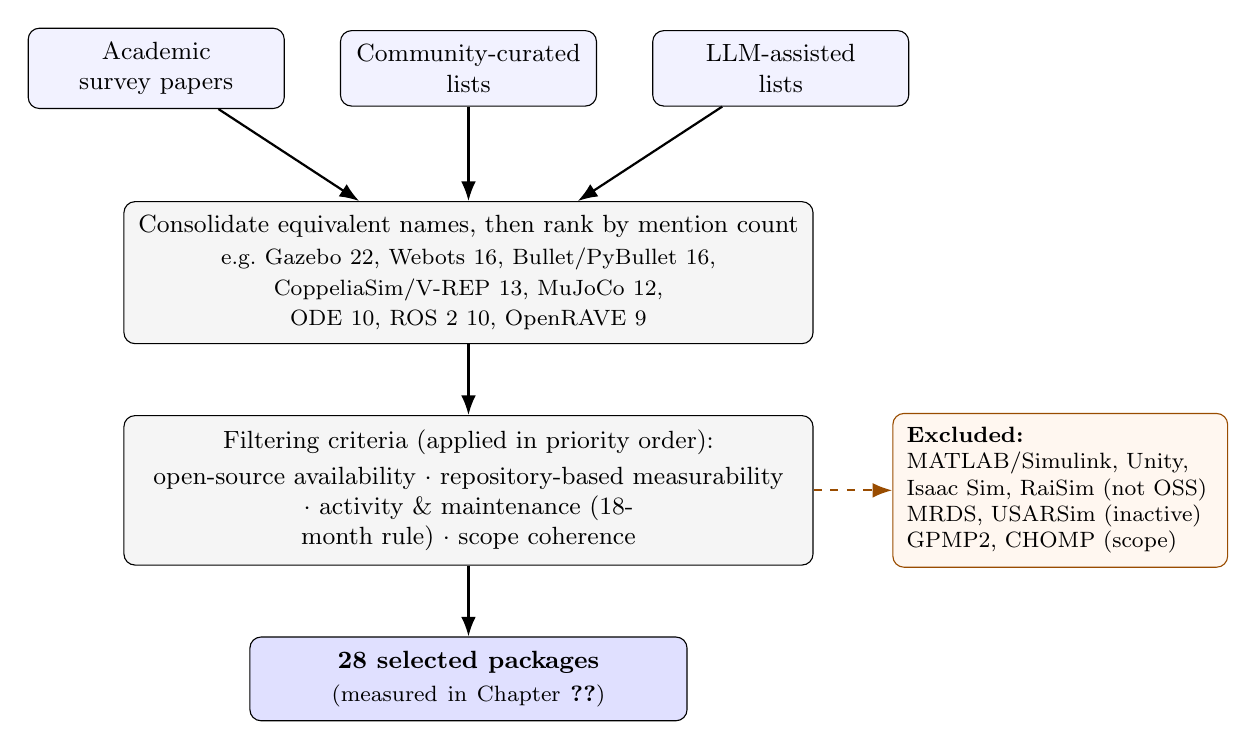
\begin{tikzpicture}[
    font=\small,
    box/.style={draw, rounded corners, align=center, inner sep=5pt, minimum height=0.85cm},
    src/.style={box, fill=blue!5, text width=2.9cm},
    proc/.style={box, fill=black!4, text width=8.4cm},
    final/.style={box, fill=blue!12, text width=5.2cm, font=\small\bfseries},
    excl/.style={box, draw=orange!60!black, fill=orange!6, align=left, text width=3.9cm, font=\footnotesize},
    arr/.style={-{Latex[length=2.5mm]}, thick},
    node distance=9mm and 7mm,
]
\node[src] (s1) {Academic\\survey papers};
\node[src, right=of s1] (s2) {Community-curated\\lists};
\node[src, right=of s2] (s3) {LLM-assisted\\lists};
\node[proc, below=12mm of s2] (cons) {Consolidate equivalent names, then rank by mention count\\[2pt]\footnotesize e.g.\ Gazebo~22, Webots~16, Bullet/PyBullet~16,\\\footnotesize CoppeliaSim/V-REP~13, MuJoCo~12, ODE~10, ROS~2~10, OpenRAVE~9};
\node[proc, below=of cons] (filt) {Filtering criteria (applied in priority order):\\[2pt]open-source availability $\cdot$ repository-based measurability\\$\cdot$ activity \& maintenance (18-month rule) $\cdot$ scope coherence};
\node[final, below=of filt] (fin) {28 selected packages\\[1pt]\footnotesize\mdseries(measured in Chapter~\ref{ch:measurement-results})};
\node[excl, right=10mm of filt] (ex) {\textbf{Excluded:}\\MATLAB/Simulink, Unity, Isaac~Sim, RaiSim (not OSS)\\MRDS, USARSim (inactive)\\GPMP2, CHOMP (scope)};
\draw[arr] (s1) -- (cons);
\draw[arr] (s2) -- (cons);
\draw[arr] (s3) -- (cons);
\draw[arr] (cons) -- (filt);
\draw[arr] (filt) -- (fin);
\draw[arr, dashed, draw=orange!60!black] (filt) -- (ex);
\end{tikzpicture}
\caption{Candidate selection pipeline. Packages discovered from three source types are consolidated and ranked by mention count, then reduced by the filtering criteria of Section~\ref{sec:filtering-criteria} to the 28 measured packages. Mention counts are source-appearance signals only (Section~\ref{sec:mention-count-ranking}); representative excluded tools and the reason for each exclusion are shown at right.}
\label{fig:candidate-selection}
\end{figure}

\begin{table}[p]
\centering
\caption{Final software set with primary roles.}
\label{tab:final-software-set}
\singlespacing
\begin{tabular}{@{}ll@{}}
\toprule
\textbf{Software} & \textbf{Primary Role} \\
\midrule
AirSim & Simulator (autonomous vehicles) \\
Bullet/PyBullet & Physics engine \\
CARLA & Simulator (autonomous driving) \\
CoppeliaSim (V-REP) & Simulator (general robotics) \\
DART & Dynamics library \\
Drake & Toolbox (dynamics, planning, control) \\
Flightmare & Simulator (quadrotor) \\
Gazebo & Simulator (general robotics) \\
GraspIt! & Manipulation (grasping) \\
Habitat & Simulator (embodied AI) \\
MORSE & Simulator (academic robotics) \\
MoveIt! & Manipulation (motion planning) \\
MRPT & Library (mobile robotics) \\
MuJoCo & Physics engine \\
Newton Dynamics & Physics engine \\
ODE (Open Dynamics Engine) & Physics engine \\
OMPL & Motion planning library \\
OpenRAVE & Planning framework \\
OpenRTM-aist & Middleware (RT components) \\
OROCOS & Control framework \\
PhysX (open-source SDK) & Physics engine \\
Pinocchio & Dynamics library \\
Project Chrono & Multi-physics simulation \\
ROS~2 & Middleware and SDK \\
Simbody & Multibody dynamics library \\
SOFA & Simulation framework \\
Webots & Simulator (general robotics) \\
YARP & Middleware (humanoid robotics) \\
\bottomrule
\end{tabular}
\end{table}

The role column is necessary because the packages are not direct substitutes. ROS~2, MoveIt!, and OMPL are boundary cases because they are not full simulators in the same sense as Gazebo or Webots; Chapter~\ref{ch:selected-software-commonality} provides the detailed category and commonality analysis used to interpret them.

\section{Measurement Procedure}
\label{sec:measurement-procedure}

The measurement procedure follows the Domain~X method for collecting structured evidence about software packages in a selected domain~\citep{Smith2021}. For each of the 28 selected packages, the study gathered source code, documentation, publications where applicable, repository metadata, issue-tracker evidence, release information, and installation evidence. The measurement record identifies the specific repository or repositories measured, since some robotics projects are distributed across multiple repositories.

\subsection{Measurement Template}
\label{subsec:measurement-template}

The primary measurement instrument is the measurement template from Appendix~B of \citet{Smith2021}; the version used in this study is reproduced in Appendix~\ref{appendix:measurement-template}. The template contains approximately 108 fields when supplementary entries (free-text ``additional comments'' fields after each section and the GitHub-style and GitStats/SCC repository metric panels) are counted alongside the substantive questions. The substantive questions are grouped into the following sections:

\begin{enumerate}
    \item \textbf{Summary Information} (17 questions): software name, URL, affiliation, purpose, number of developers, funding, initial release date, last commit date, status, license, platforms, software category, development model, publications, source code URL, programming languages, and evidence of performance consideration.
    \item \textbf{Installability} (14 questions): installation instructions (presence, single-document organization, linear ordering, completeness, and assumed pre-installed dependencies), compatible operating system versions, installation automation, error handling, installation validation procedure, number of installation steps, operating system used during measurement, dependencies (presence of guidance and required version listing), and uninstall behaviour (problems and residue).
    \item \textbf{Correctness and Verifiability} (8 questions): requirements or theory documentation, correctness techniques, tutorial availability and quality, unit tests, and continuous integration evidence.
    \item \textbf{Surface Reliability} (5 questions): installation and tutorial breakage, error messages, and recoverability.
    \item \textbf{Surface Robustness} (2 questions): handling of unexpected input and edge cases.
    \item \textbf{Surface Usability} (4 questions): tutorial, user manual, user characteristics, support model.
    \item \textbf{Maintainability} (7 questions): version number, contribution guidance, available artifacts, issue tracking, issue closure rate, comment percentage, and version control.
    \item \textbf{Reusability} (2 questions): number of code files and API documentation.
    \item \textbf{Surface Understandability} (8 questions): code formatting, coding standards, identifier quality, constant usage, comment clarity, algorithm references, parameter ordering, and modularization.
    \item \textbf{Visibility and Transparency} (4 questions): development process definition, process documentation, development environment documentation, and release notes.
\end{enumerate}

Applying the same template to every package ensures that comparisons are based on a consistent set of observations rather than ad hoc impressions. Each quality section concludes with an overall impression score on a scale of 1 to 10, assigned using the scoring guidelines of the impression calculator in Appendix~C of \citet{Smith2021}. The impression scores summarize more than the recorded checklist answers alone: they also reflect observations made during measurement, such as the quality and currency of documentation, the clarity of error messages, and the overall installation and tutorial experience, which the mostly binary checklist fields do not capture. Two packages with identical checklist answers can therefore receive different impression scores; Chapter~\ref{ch:threats-to-validity} discusses the subjectivity this introduces.

\subsection{Repository Metrics}
\label{subsec:repository-metrics}

Repository metrics are collected separately from the quality impression scores. Three categories of repository data are gathered:

\begin{enumerate}
    \item \textbf{GitHub-style metrics:} stars, forks, watchers, open pull requests, closed pull requests, number of developers, open issues, closed issues, initial release date, and last commit date.
    \item \textbf{GitStats-style metrics:} number of text-based files, number of binary files, total lines, lines added, lines deleted, total commits, commits by year (last 5 years), and commits by month (last 12 months).
    \item \textbf{SCC-style metrics:} number of text-based files, total lines, code lines, comment lines, and blank lines.
\end{enumerate}

From these raw data, three processed measures are calculated:

\begin{enumerate}
    \item \textbf{Alive/dead status:} alive is defined as the presence of commits or version releases within the last 18 months from the measurement date.
    \item \textbf{Percentage of identified issues that are closed:} computed as closed issues divided by total identified issues.
    \item \textbf{Percentage of code that is comments:} computed as comment lines divided by total lines.
\end{enumerate}

\subsection{Measurement Execution}
\label{subsec:measurement-execution}

The Domain~X methodology recommends performing installation-based measurements in a controlled environment, typically a virtual machine, to ensure a clean and reproducible starting state~\citep{Smith2021}. For this report, installation measurements were performed on a Linux-based virtual machine. The operating system, installation steps, dependencies, and any issues encountered were recorded for each package.

The methodology also recommends a time budget to keep the overall measurement workload feasible. The full assessment is estimated at roughly 173 person-hours per domain, against a stated goal of about one person-month (160 hours), with 1 to 4 hours allocated per package for template completion and up to 2 hours for installation~\citep{Smith2021}. Measurement was conducted during May 2026. All time-sensitive data (last commit dates, issue counts, stars, forks, etc.) should be understood as snapshots taken during this period.

Several measurement questions require explicit interpretation rules:

\begin{itemize}
    \item \textbf{Last commit date} is recorded at the time of measurement and may change for active repositories.
    \item \textbf{Percentage of identified issues that are closed} is computed consistently as closed issues divided by total identified issues, using GitHub issue data where available.
    \item \textbf{Evidence that performance was considered} is assessed by searching software artifacts for explicit references to speed, storage, throughput, performance optimization, parallelism, multi-core processing, or similar considerations.
    \item \textbf{Percentage of code that is comments} is computed using the SCC tool's line-based method, as comment lines divided by total lines.
\end{itemize}

\subsection{Ranking with AHP}
\label{subsec:ahp-ranking}

After the quality measures are collected, the Domain~X methodology uses the Analytic Hierarchy Process (AHP) to support ranking across the nine quality categories~\citep{Saaty1980}. AHP is a decision-making technique that uses pairwise comparisons between alternatives to calculate relative scores. It organizes multiple criteria in a hierarchical structure and enables the combination of individual quality rankings into an overall ranking based on the relative priorities assigned to each quality.

In this report, AHP would be applied to the nine quality impression scores for the 28 software packages and would produce a ranking that depends on the chosen criterion weights. Sensitivity analysis would then assess whether the ranking is stable under reasonable variations in those weights. An elicited-weight AHP ranking is not computed here, because a defensible criterion-weighting elicitation has not been completed at the time of writing; Chapter~\ref{ch:measurement-results} therefore reports the per-package quality-mean ranking and a comparison with community indicators, together with an illustrative equal-weight AHP computation that demonstrates the weighting step.

\section{Commonality Analysis Procedure}
\label{sec:commonality-analysis-procedure}

The commonality analysis identifies shared and variable capabilities across the selected software packages, treating them as members of a software family as defined by \citet{Parnas1976} and \citet{Weiss1998}. The analysis supplements repository-based metrics by describing what the packages do and how their roles differ, providing context for interpreting the measurement results reported in Chapter~\ref{ch:measurement-results}.

Following the Domain~X methodology, the analysis proceeds in six steps:

\begin{enumerate}
    \item \textbf{Write an introduction} to the domain and the software family.
    \item \textbf{Write an overview of domain knowledge,} summarizing the key concepts and terminology relevant to MPS software.
    \item \textbf{List commonalities:} identify goals, assumptions, functions, artifacts, and domain concepts that recur across multiple family members. For example, many of the selected packages share the goal of simulating robot dynamics, the assumption that robot models are described using standard formats (such as URDF or SDF), and the function of providing an API for programmatic control.
    \item \textbf{List variabilities:} identify dimensions on which family members differ. These include software role (simulator, physics engine, planning library, middleware), supported platforms, licensing, programming language interfaces, documentation style, and intended use cases.
    \item \textbf{List parameters of variation:} for each variability, describe the possible values. For example, the software role parameter can take values such as general-purpose simulator, domain-specific simulator, physics engine, dynamics library, motion planning library, manipulation framework, or middleware.
    \item \textbf{Add terminology, definitions, and acronyms} that are standard in the domain, to ensure that the analysis is accessible to readers outside robotics.
\end{enumerate}

The procedure first groups the selected packages into broad categories based on their primary roles: robotics simulators, physics and dynamics engines, and planning or middleware tools. It then identifies capabilities that appear across multiple categories, such as support for robot model representation, simulated environments, motion planning workflows, dynamics computation, and integration with robotics ecosystems.

Because the selected packages span multiple roles, the commonality analysis does not force all tools into a single comparison template. Its purpose is to describe shared concerns and meaningful differences, not to claim that every package provides identical functionality. The analysis is based on checked evidence from documentation, repositories, publications, and other reliable project materials. Capabilities that could not be verified against these materials are not reported.

\section{Interview Component}
\label{sec:interview-component}

The Domain~X methodology includes a developer survey component designed to capture information that is not visible in public repositories: the development process as experienced by practitioners, the pain points they encounter, their perceptions of software quality threats, and the strategies they use to address those threats~\citep{Smith2021}. The methodology prescribes semi-structured interviews based on a list of 20 questions covering developer background, project organization, user understanding, development obstacles (past and present), documentation practices, and specific software qualities including maintainability, understandability, usability, and reproducibility.

For this report, the interview component requires research ethics approval from the McMaster Research Ethics Board (MREB), with the application submitted through the MacREM online system, before recruitment or data collection. The planned interview participants are software developers, maintainers, or programmers associated with the studied packages. Approved ethics materials and the interview protocol will be archived in Appendix~\ref{appendix:interview-materials}.

Chapter~\ref{ch:developer-interviews} records the planned reporting structure for the interview component. Until ethics approval, recruitment, and analysis are complete, that chapter does not report developer findings; it identifies RQ6--RQ9 as questions that require interview evidence.

The methodology recommends sending interview requests to developers from all packages in the study set to avoid selection bias. Prior applications of the methodology report response rates roughly in the 15\%--30\% range~\citep{Smith2021,Smith2024MI}; the exact rate for this report will depend on outreach timing and the response practices of the contacted developers. Interview contacts are typically identified through project websites, code repositories, publications, or institutional biography pages.

        \setcounter{figure}{0}
        \setcounter{equation}{0}
        \setcounter{table}{0}

  \chapter{Selected Software and Commonality Analysis}
\label{ch:selected-software-commonality}

This chapter characterizes the final 28 packages (Section~\ref{sec:final-software-set}) for RQ1 and gives the commonality context used later when interpreting the RQ2 measurements. The commonality analysis follows the \citet{Weiss1998} procedure described in Section~\ref{sec:commonality-analysis-procedure}; capabilities are reported only where they could be verified against the project materials.

\section{Overview of Selected Software}
\label{sec:overview-selected-software}

The selected packages come from a mix of development settings---academic research groups, open-source foundations and companies, corporate research labs, and smaller communities or individual maintainers---detailed under V9 (Section~\ref{sec:variabilities}).

The packages span a period of active development from 2001 (ODE's initial release) to the present, with most showing recent repository activity as of the May 2026 measurement date. Licensing, language, and platform details are reported with the measurement data in Section~\ref{sec:repository-project-metadata} (Table~\ref{tab:summary-metadata}).

\section{Functional Software Roles}
\label{sec:robotics-software-categories}

The selected packages can be grouped into three broad functional roles by their primary function in a robotics workflow. These roles are not strict boundaries---some packages span several (see Section~\ref{sec:boundary-cases})---but they structure the commonality analysis.

\subsection{Robotics Simulators}
\label{subsec:robotics-simulators}

Robotics simulators provide virtual environments for representing robots, worlds, sensors, and actuators, letting users test algorithms, validate designs, and collect synthetic data before deploying to hardware. They typically offer graphical rendering, physics simulation, sensor models, and programmatic interfaces for controlling simulated robots. The selected packages primarily classified as simulators are:

\begin{itemize}
    \item \textbf{Gazebo} (including the Ignition/Gazebo Sim lineage) is a long-established open-source 3D robotics simulator developed by Open Robotics. It provides physics simulation through multiple backends, rendering, sensor models, and ROS integration.
    \item \textbf{Webots} is a multi-platform robot simulator maintained by Cyberbotics. It supports modelling, programming, and simulating robots, vehicles, and mechanical systems, with a large library of pre-built robot models.
    \item \textbf{CoppeliaSim} (formerly V-REP) is a versatile robot simulation framework developed by Coppelia Robotics. It supports rapid algorithm development, factory automation simulation, prototyping, verification, and digital twin applications.
    \item \textbf{AirSim} is an open-source simulator for autonomous vehicles (drones and ground vehicles) built on Unreal Engine and developed by Microsoft Research. Its repository-activity classification and officially discontinued status are discussed in Section~\ref{subsec:activity-maintenance-status}.
    \item \textbf{CARLA} is an open-source autonomous driving simulator built on Unreal Engine and developed by the Computer Vision Center in Barcelona and Intel. It provides photorealistic urban environments and a broad sensor suite for autonomous driving research.
    \item \textbf{MORSE} (Modular OpenRobots Simulation Engine) is a generic academic robotic simulator based on Blender and the Bullet physics engine, designed to remain middleware-agnostic across ROS, YARP, and other frameworks.
    \item \textbf{Habitat} is a 3D simulator for embodied AI research developed by Meta AI Research. It supports training and evaluation of embodied AI agents in photorealistic indoor environments.
    \item \textbf{Flightmare} is a flexible modular quadrotor simulator developed by the Robotics and Perception Group at the University of Zurich and ETH Zurich. It separates rendering from the RL environment for flexible configuration between fast and photorealistic modes.
\end{itemize}

Drake, MRPT, and SOFA also provide simulation capabilities as part of broader roles (Section~\ref{sec:boundary-cases}).

\subsection{Physics Engines and Dynamics Libraries}
\label{subsec:physics-engines-dynamics-libraries}

Physics engines and dynamics libraries provide the computational foundation for simulating rigid-body and multibody dynamics, collision detection, and contact resolution. They often serve as backends to higher-level simulators but can also be used directly. The selected packages primarily classified as physics engines or dynamics libraries are:

\begin{itemize}
    \item \textbf{Bullet/PyBullet} is a widely used open-source physics engine for simulation, robotics, and deep reinforcement learning. PyBullet provides Python bindings that have made it popular in the machine learning community.
    \item \textbf{MuJoCo} (Multi-Joint dynamics with Contact) is a general-purpose physics simulator maintained by Google DeepMind. It is designed for fast and accurate simulation of articulated structures and is widely used in robotics and reinforcement learning research.
    \item \textbf{ODE} (Open Dynamics Engine) is one of the earliest open-source libraries for simulating rigid body dynamics. It has been used extensively in robotics and served as a physics backend for Gazebo Classic.
    \item \textbf{PhysX} is NVIDIA's real-time physics engine SDK. The open-source SDK provides capabilities for simulating rigid bodies, particles, vehicles, and deformable bodies, primarily targeted at real-time simulation applications.
    \item \textbf{DART} (Dynamic Animation and Robotics Toolkit) is a C++ physics engine and kinematics/dynamics library developed at Georgia Tech and other institutions. It is designed for stable simulation in manipulation and locomotion research.
    \item \textbf{Simbody} is a multibody dynamics library developed at Stanford University for simulating articulated biomechanical and mechanical systems. It is the physics engine underlying OpenSim (biomedical simulation software).
    \item \textbf{Pinocchio} is a fast and flexible C++ library for rigid-body dynamics computations and their analytical derivatives, developed primarily at Inria and LAAS-CNRS. It implements state-of-the-art algorithms for kinematics, dynamics, and Jacobians.
    \item \textbf{Project Chrono} is an open-source multi-physics simulation library developed at the University of Wisconsin-Madison and the University of Parma. It supports multibody dynamics, finite element analysis, vehicle dynamics, and GPU-accelerated simulation.
    \item \textbf{Newton Dynamics} is a cross-platform physics simulation engine optimized for real-time deterministic rigid-body simulation. It is used in game development and robotics simulation.
    \item \textbf{SOFA} (Simulation Open Framework Architecture) is an open-source real-time simulation framework developed primarily at Inria. It focuses on deformable object simulation, finite element methods, and haptic feedback, with applications in surgical simulation and soft robotics.
\end{itemize}

\subsection{Motion Planning, Middleware, and Manipulation Packages}
\label{subsec:motion-planning-middleware-manipulation}

Motion planning libraries, robotics middleware, and manipulation packages cover parts of the workflow outside full-world simulation: planning algorithms, communication layers, grasp planning, and system integration. They are included because MPS workflows typically combine planning, simulation, and execution rather than using simulators alone. The selected packages primarily classified as planning or middleware packages are:

\begin{itemize}
    \item \textbf{ROS~2} (Robot Operating System 2) is an open-source software development kit and middleware framework for building robot applications. It provides communication infrastructure (based on DDS), hardware abstraction, drivers, libraries, visualization tools, and a large ecosystem of community packages. ROS~2 is the successor to ROS~1 and represents a major redesign with emphasis on real-time control, multi-robot deployment, and production use.
    \item \textbf{MoveIt!} refers to the active MoveIt~2 generation for ROS~2 in this report. It is an open-source robotics manipulation framework that provides motion planning, kinematics, collision checking, trajectory execution, and perception integration for robot arms and manipulators, integrating OMPL and other planners as plugins.
    \item \textbf{OMPL} (Open Motion Planning Library) is an open-source C++ library for sampling-based motion planning algorithms developed at Rice University. It provides implementations of widely used planners such as PRM, RRT, RRT*, and EST, and is the default planning backend for MoveIt!.
    \item \textbf{OpenRAVE} (Open Robotics Automation Virtual Environment) is an open-source robotics planning framework focused on simulation and analysis of kinematic and geometric information for motion planning, particularly for manipulation tasks.
    \item \textbf{Drake} is an open-source C++ and Python toolbox for model-based design and verification of robotics systems, developed by MIT and the Toyota Research Institute (TRI). It covers multibody dynamics, trajectory optimization, model predictive control, perception, and manipulation planning.
    \item \textbf{OROCOS} (Open RObot COntrol Software) is an open-source C++ framework for real-time robot control developed at KU Leuven. Its major components include the Real-Time Toolkit for component-based hard real-time software and the Kinematics and Dynamics Library.
    \item \textbf{MRPT} (Mobile Robot Programming Toolkit) is an open-source cross-platform C++ library for mobile robotics research, providing algorithms for SLAM, computer vision, motion planning, and sensor data processing.
    \item \textbf{YARP} (Yet Another Robot Platform) is open-source middleware for humanoid and general robotics, developed at the Istituto Italiano di Tecnologia. It provides communication infrastructure for distributed robot systems and is the primary middleware for the iCub humanoid robot platform.
    \item \textbf{OpenRTM-\allowbreak aist} implements the OMG Robot Technology Component standard and was developed at AIST in Japan. It provides a component-based framework for creating and connecting robot software modules.
    \item \textbf{GraspIt!} is a simulation environment for robotic grasping research developed at Columbia University. It supports loading robot hand models and 3D object models to plan, evaluate, and visualize grasps.
\end{itemize}

\section{Family and Sub-family Commonalities}
\label{sec:commonalities}

For this analysis, a commonality must hold at the level where it is claimed. A family-wide commonality must hold for every member of the 28-package study set; a feature shared only by one role group is stated as a sub-family commonality; and a feature whose values differ across packages is treated as a variability. This layered structure follows the role grouping in Section~\ref{sec:robotics-software-categories} and avoids presenting a simulator property as if it also characterized middleware or a focused planning library. Figure~\ref{fig:feature-model} summarizes the resulting structure.

\begin{figure}[htbp]
\centering
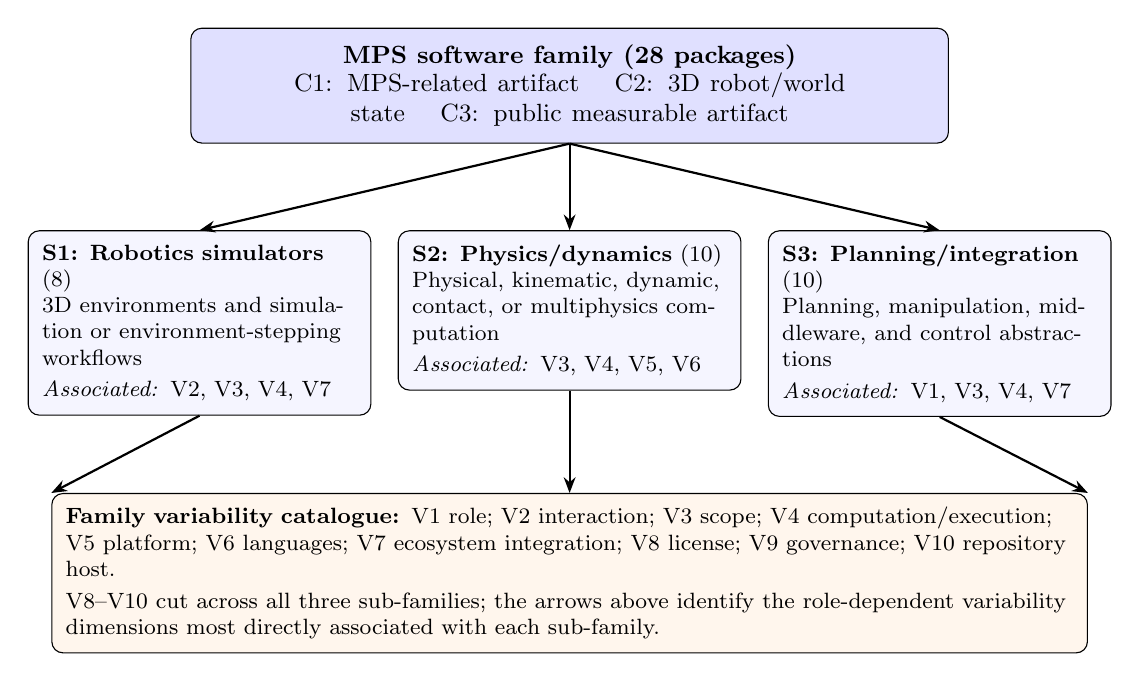
\begin{tikzpicture}[
  font=\footnotesize,
  root/.style={draw, rounded corners, fill=blue!12, font=\small\bfseries, inner sep=6pt, align=center, text width=9.2cm},
  sub/.style={draw, rounded corners, fill=blue!4, align=left, inner sep=5pt, text width=4.0cm},
  var/.style={draw, rounded corners, fill=orange!7, align=left, inner sep=5pt, text width=12.8cm},
  arr/.style={-{Stealth[length=2mm]}, thick},
]
\node[root] (root) {MPS software family (28 packages)\\[-1pt]
\mdseries C1: MPS-related artifact \quad C2: 3D robot/world state \quad C3: public measurable artifact};
\node[sub, below=11mm of root, xshift=-4.7cm] (s1) {\textbf{S1: Robotics simulators} (8)\\
3D environments and simulation or environment-stepping workflows\\[2pt]
\textit{Associated:} V2, V3, V4, V7};
\node[sub, below=11mm of root] (s2) {\textbf{S2: Physics/dynamics} (10)\\
Physical, kinematic, dynamic, contact, or multiphysics computation\\[2pt]
\textit{Associated:} V3, V4, V5, V6};
\node[sub, below=11mm of root, xshift=4.7cm] (s3) {\textbf{S3: Planning/integration} (10)\\
Planning, manipulation, middleware, and control abstractions\\[2pt]
\textit{Associated:} V1, V3, V4, V7};
\node[var, below=13mm of s2] (vars) {\textbf{Family variability catalogue:}
V1 role; V2 interaction; V3 scope; V4 computation/execution; V5 platform; V6 languages; V7 ecosystem integration; V8 license; V9 governance; V10 repository host.\\[2pt]
V8--V10 cut across all three sub-families; the arrows above identify the role-dependent variability dimensions most directly associated with each sub-family.};
\draw[arr] (root.south) -- (s1.north);
\draw[arr] (root.south) -- (s2.north);
\draw[arr] (root.south) -- (s3.north);
\draw[arr] (s1.south) -- (vars.north west);
\draw[arr] (s2.south) -- (vars.north);
\draw[arr] (s3.south) -- (vars.north east);
\end{tikzpicture}
\caption{Relationship between the MPS family, its three role-based sub-families, and the ten variability dimensions. The sub-family boxes identify their most direct role-dependent variabilities; V8--V10 apply across all three groups.}
\label{fig:feature-model}
\end{figure}

\textbf{C1: MPS-related software artifact.} Every selected package performs at least one task in an MPS workflow: planning, simulation, dynamics, control, manipulation, or integration. This is the top-level commonality. The packages are not interchangeable, but each belongs to the domain this thesis studies, and the sub-families below (with V1--V4) record the different roles they play.

\textbf{C2: Three-dimensional robot or world state.} Every selected package supports three-dimensional robot or environment state. Simulators and physics libraries provide 3D geometry, kinematics, and dynamics directly; planning and manipulation software plans in 3D configuration spaces or workspaces, even when, as in OMPL, the underlying algorithms are dimension-agnostic; middleware carries 3D pose and transform data. How this state is used differs (V3, V4), but support for three dimensions is universal. The one two-dimensional candidate considered, Player/Stage, was not selected (Appendix~\ref{appendix:full-candidate-software-list}).

\textbf{C3: Public measurable technical artifact.} Every package has a public source repository and enough user-facing documentation to be measured. The measurement records confirm a documented API, installation instructions, a getting-started tutorial, and a user manual for all 28 packages. This commonality is partly a product of the selection criteria (Section~\ref{subsec:repository-based-measurability}); it does not mean that all MPS software is equally open or equally documented. License (V8), governance (V9), and repository host (V10) remain variable.

The three sub-families in Table~\ref{tab:subfamily-commonalities} make the role-specific commonalities explicit. These commonalities should not be read as claims about all 28 packages; they hold within the stated sub-family and become variabilities when the whole family is compared.

\begin{table}[H]
\centering
\caption{Sub-family commonalities and associated variabilities.}
\label{tab:subfamily-commonalities}
\singlespacing
\footnotesize
\setlength{\tabcolsep}{2.5pt}
\begin{tabular}{@{}P{2.4cm}P{3.8cm}P{4.3cm}P{2.4cm}@{}}
\toprule
\textbf{Sub-family} & \textbf{Members} & \textbf{Sub-family commonalities} & \textbf{Associated variabilities} \\
\midrule
S1: Robotics simulators & AirSim, CARLA, CoppeliaSim, Flightmare, Gazebo, Habitat, MORSE, Webots & Provide 3D virtual environments for representing robots, worlds, sensors, or agents; support a simulation or environment-stepping workflow used for testing, data generation, or algorithm development. & Interaction mode (V2), application scope (V3), computation/execution model (V4), ecosystem integration (V7) \\
\hline
S2: Physics engines and dynamics libraries & Bullet/PyBullet, DART, MuJoCo, Newton Dynamics, ODE, PhysX, Pinocchio, Project Chrono, Simbody, SOFA & Compute physical, kinematic, or dynamic properties of bodies, articulated systems, contacts, or deformable/multiphysics models; expose solver or library interfaces for use directly or as backends. & Application scope (V3), computation model (V4), platform support (V5), programming languages (V6) \\
\hline
S3: Planning, middleware, and manipulation software & Drake, GraspIt!, MoveIt!, MRPT, OMPL, OpenRAVE, OpenRTM-\allowbreak aist, OROCOS, ROS~2, YARP & Expose reusable application-level robotics abstractions rather than standalone physics backends. Planning and manipulation packages express these abstractions as motions and grasps; middleware and control packages express them as components, devices, controllers, and messages. & Primary role (V1), application scope (V3), computation/execution model (V4), ecosystem integration (V7) \\
\bottomrule
\end{tabular}
\end{table}

\section{Variabilities}
\label{sec:variabilities}

The family-wide and sub-family commonalities above are realized differently across the selected packages. The ten variability dimensions below include role-specific patterns such as physics or kinematics computation, ecosystem integration, and simulation or planning loops. These patterns are common within some sub-families but are variabilities at the level of the full 28-package family.

\textbf{V1: Primary Software Role.} The most fundamental variability is the role a package plays in a robotics workflow, ranging from full simulation environments to physics engines to planning libraries to middleware frameworks (Section~\ref{sec:robotics-software-categories}).

\textbf{V2: Interaction Mode.} Some packages combine a graphical environment with a programmatic API (Gazebo, Webots, and CoppeliaSim), whereas focused libraries are primarily API-driven (OMPL, Pinocchio, and ODE). This variability describes the user-facing interaction mode, not the C3 measurement baseline that all selected packages provide enough technical material to be studied.

\textbf{V3: Application Scope.} General-purpose robotics simulators and engines coexist with packages specialized for autonomous driving, aerial vehicles, embodied AI, medical or soft robotics, grasping, mobile robotics, manipulation, and real-time control (Section~\ref{sec:robotics-software-categories}).

\textbf{V4: Computation or Execution Model.} The software may implement a time-stepped simulation loop, a dynamics or kinematics solver, a planning or optimization pipeline, a middleware/component runtime, or several of these models in one toolbox. This variability captures capabilities that are common within some sub-families, such as physics computation and iterative simulation or planning loops, but not across all 28 packages.

\textbf{V5: Platform Support.} All packages support Linux, and support for other platforms varies. Some packages provide first-class support for Windows and macOS (Webots, CoppeliaSim, Bullet), while others are primarily developed for Linux with limited cross-platform support.

\textbf{V6: Recorded Programming Languages.} C++ and Python are the dominant languages in the measurement records, but the recorded sets differ. Some packages use C or C++ without Python, many pair C++ with Python, and larger frameworks record additional languages such as Java, MATLAB, or IDL. This variability reports the languages in the measurement dataset; it does not infer a public API from repository language counts.

\textbf{V7: Robotics-Ecosystem Integration.} MoveIt! is ROS-native, Gazebo is closely ROS-integrated, and simulators such as Webots and CARLA provide bridges. MORSE supports several middleware systems. YARP, OROCOS, and OpenRTM-\allowbreak aist provide alternative middleware or component models, while other libraries are usable independently. Ecosystem integration is therefore a variability with native, bridge, multi-middleware, alternative-middleware, and standalone values.

\textbf{V8: License Model.} The measured source artifacts use permissive, reciprocal, dual, and mixed distribution models. CoppeliaSim is the principal mixed-model case because the measured GPL source coexists with commercial and educational distribution licences. License choice affects how software can be redistributed and integrated.

\textbf{V9: Governance Model.} Governance ranges across companies, open-source foundations, academic or public research institutions, mixed consortia, and independent communities or maintainers. The categories describe the primary stewardship visible in the measurement snapshot rather than legal ownership of every component.

\textbf{V10: Repository Host.} GitHub hosts the measured source for 27 packages. ODE is the exception: its primary repository is on Bitbucket, with a GitHub mirror also recorded. The commonality is public Git-based measurability (C3), while the hosting service is variable.

\section{Parameters of Variation}
\label{sec:parameters-of-variation}

For each variability identified in Section~\ref{sec:variabilities}, Table~\ref{tab:parameters-of-variation} summarizes the parameters of variation and their typical binding times (defined in Section~\ref{sec:commonality-analysis-background}). Binding time records when a value is fixed for a package or selected by an integrator; it is not the date on which the measurement was collected.

\begin{table}[H]
\centering
\caption{Parameters of variation and binding times.}
\label{tab:parameters-of-variation}
\singlespacing
\small
\begin{tabular}{@{}P{3.2cm}P{7.1cm}P{3.0cm}@{}}
\toprule
\textbf{Variability} & \textbf{Parameters of Variation} & \textbf{Binding Time} \\
\midrule
V1: Primary role & Simulator; physics/dynamics engine, library, or framework; planning or manipulation library/framework; middleware or control framework; multi-purpose or multiphysics package & Specification time \\
\hline
V2: Interaction mode & Graphical plus API, primarily API & Specification / run time \\
\hline
V3: Application scope & General robotics/physics; autonomous vehicles; aerial vehicles; embodied AI; medical/soft robotics; grasping; mobile robotics; motion/manipulation planning; real-time control; rigid-body, multibody, or multiphysics applications & Specification time \\
\hline
V4: Computation/execution & Simulation loop; dynamics or kinematics solver; planning, search, or optimization pipeline; middleware/component runtime; combined planning/simulation, dynamics/simulation, component/kinematics, or multi-role model & Specification / configuration time \\
\hline
V5: Platform support & Linux, with the measured combinations of Windows, macOS, Android, or BSD support & Specification / build time \\
\hline
V6: Recorded languages & C++; C/C++; C/Python; C++/Python; multi-language; unclear in the measurement record & Build / configuration time \\
\hline
V7: Ecosystem integration & ROS-native/integrated, ROS bridge, multi-middleware, alternative middleware/component model, standalone & Build / configuration / run time \\
\hline
V8: License & Specific permissive, reciprocal, dual, or mixed open-source/commercial licence recorded in the sub-family package maps below & Specification time \\
\hline
V9: Governance & Company, foundation, academic/public institution, mixed consortium, independent/community & Specification time \\
\hline
V10: Repository host & GitHub, Bitbucket with GitHub mirror & Specification time \\
\bottomrule
\end{tabular}
\end{table}

The binding times reflect when a user or integrator can still make a choice. Roles, governance, and repository hosting are fixed at specification or project-organization time, whereas ecosystem integration may also be selected when a package is built, configured, or connected at run time.

Tables~\ref{tab:simulator-variability-map}--\ref{tab:planning-variability-map} map all ten variabilities at package level, one table per sub-family. This arrangement keeps a package's functional, delivery, and governance values in one row. The values synthesize the final-set roles in Table~\ref{tab:final-software-set}, the metadata in Table~\ref{tab:summary-metadata}, and the package purposes in the measurement dataset; they are descriptive, not quality scores.

For compactness, L, W, M, A, and B denote Linux, Windows, macOS, Android, and BSD; GH and BB denote GitHub and Bitbucket; and MW denotes middleware. V7 distinguishes ROS-native or closely integrated software, optional ROS bridges, multi-middleware support, alternative middleware/component models, and standalone use.

\newcommand{\variationmapheader}{%
\toprule
\textbf{Software} & \textbf{V1 Role} & \textbf{V2 Interact.} & \textbf{V3 Scope} & \textbf{V4 Execution} & \textbf{V5 Platform} & \textbf{V6 Languages} & \textbf{V7 Integration} & \textbf{V8 License} & \textbf{V9 Governance} & \textbf{V10 Host} \\
\midrule}

\begin{landscape}
\begin{table}[H]
\centering
\caption{Complete V1--V10 package map for S1: robotics simulators.}
\label{tab:simulator-variability-map}
\begingroup
\singlespacing
\fontsize{7pt}{8.2pt}\selectfont
\setlength{\tabcolsep}{1.2pt}
\begin{tabular}{@{}P{2.0cm}P{2.2cm}P{1.25cm}P{2.15cm}P{2.35cm}P{1.35cm}P{1.65cm}P{1.65cm}P{1.4cm}P{1.65cm}P{1.05cm}@{}}
\variationmapheader
AirSim & Simulator & GUI + API & Autonomous vehicles & Simulation loop & L/W & C++/\allowbreak{}Python & ROS bridge & MIT & Company & GH \\
CARLA & Simulator & GUI + API & Autonomous driving & Simulation loop & L/W & C++/\allowbreak{}Python & ROS bridge & MIT & Mixed consortium & GH \\
CoppeliaSim & Simulator & GUI + API & General robotics & Simulation loop & L/W/M & C++/\allowbreak{}Python & ROS bridge & GPL + commercial & Company & GH \\
Flightmare & Simulator & GUI + API & Aerial vehicles & Simulation loop & L & C++/\allowbreak{}Python & Standalone & MIT & Academic & GH \\
Gazebo & Simulator & GUI + API & General robotics & Simulation loop & L/W/M & C++/\allowbreak{}Python & ROS integrated & Apache-2.0 & Foundation & GH \\
Habitat & Simulator & API & Embodied AI & Simulation loop & L/M & C++/\allowbreak{}Python & Standalone & MIT & Company & GH \\
MORSE & Simulator & GUI + API & General robotics & Simulation loop & L/W/M & C/\allowbreak{}Python & Multi-MW & BSD & Academic & GH \\
Webots & Simulator & GUI + API & General robotics & Simulation loop & L/W/M & Multi-language & ROS bridge & Apache-2.0 & Company & GH \\
\bottomrule
\end{tabular}
\endgroup
\end{table}
\end{landscape}

\begin{landscape}
\begin{table}[H]
\centering
\caption{Complete V1--V10 package map for S2: physics engines and dynamics libraries.}
\label{tab:physics-variability-map}
\begingroup
\singlespacing
\fontsize{7pt}{8.2pt}\selectfont
\setlength{\tabcolsep}{1.2pt}
\begin{tabular}{@{}P{2.0cm}P{2.2cm}P{1.25cm}P{2.15cm}P{2.35cm}P{1.35cm}P{1.65cm}P{1.65cm}P{1.4cm}P{1.65cm}P{1.05cm}@{}}
\variationmapheader
Bullet/PyBullet & Physics engine & API & General physics/robotics & Dynamics solver & L/W/M & C++/\allowbreak{}Python & Standalone & zlib & Community & GH \\
DART & Dynamics library & API & General robotics/\allowbreak{}dynamics & Dynamics/kinematics solver & L/W/M/\allowbreak{}B & C++/\allowbreak{}Python & Standalone & BSD & Academic & GH \\
MuJoCo & Physics engine & GUI + API & General physics/robotics & Dynamics solver & L/W/M & C++/\allowbreak{}Python & Standalone & Apache-2.0 & Company & GH \\
Newton Dynamics & Physics engine & API & General physics & Dynamics solver & L/W/M/\allowbreak{}A & C/\allowbreak{}C++ & Standalone & zlib & Independent & GH \\
ODE & Physics engine & API & General physics & Dynamics solver & L/W/M & Unclear & Standalone & BSD/\allowbreak{}LGPL & Independent & BB + GH \\
PhysX & Physics engine & API & General physics & Dynamics solver & L/W & C++ & Standalone & BSD & Company & GH \\
Pinocchio & Dynamics library & API & Rigid-body robotics & Dynamics/kinematics solver & L/W/M & C++/\allowbreak{}Python & Standalone & BSD & Academic & GH \\
Project Chrono & Multi-physics simulation & API & Multiphysics/vehicles & Dynamics/simulation & L/W/M & C++/\allowbreak{}Python & Standalone & BSD & Academic & GH \\
Simbody & Dynamics library & API & Multibody/\allowbreak{}biomechanics & Dynamics solver & L/W/M & C/\allowbreak{}C++ & Standalone & Apache-2.0 & Academic & GH \\
SOFA & Simulation framework & GUI + API & Medical/soft robotics & Simulation loop & L/W/M & C++/\allowbreak{}Python & Standalone & LGPL-2.1 & Academic & GH \\
\bottomrule
\end{tabular}
\endgroup
\end{table}
\end{landscape}

\begin{landscape}
\begin{table}[H]
\centering
\caption{Complete V1--V10 package map for S3: planning, middleware, and manipulation software.}
\label{tab:planning-variability-map}
\begingroup
\singlespacing
\fontsize{7pt}{8.2pt}\selectfont
\setlength{\tabcolsep}{1.2pt}
\begin{tabular}{@{}P{2.0cm}P{2.2cm}P{1.25cm}P{2.15cm}P{2.35cm}P{1.35cm}P{1.65cm}P{1.65cm}P{1.4cm}P{1.65cm}P{1.05cm}@{}}
\variationmapheader
Drake & Multi-purpose toolbox & API & General robotics & Multi-role & L/M & C++/\allowbreak{}Python & Standalone & BSD & Mixed consortium & GH \\
GraspIt! & Manipulation framework & GUI + API & Robotic grasping & Planning/simulation & L/W/M & C/\allowbreak{}C++/\allowbreak{}IDL & Standalone & GPL v3+ & Academic & GH \\
MoveIt! & Manipulation framework & GUI + API & Manipulation & Planning pipeline & L & C++/\allowbreak{}Python & ROS native & BSD & Mixed consortium & GH \\
MRPT & Multi-purpose library & GUI + API & Mobile robotics & Multi-role & L/W/M & C++/\allowbreak{}Python & ROS bridge & BSD & Academic & GH \\
OMPL & Motion planning library & API & Motion planning & Planning/search & L/W/M & C++/\allowbreak{}Python & Standalone & BSD & Academic & GH \\
OpenRAVE & Planning framework & GUI + API & Manipulation/planning & Planning pipeline & L/W/M & C++/\allowbreak{}Python & ROS bridge & LGPL/\allowbreak{}A2.0 & Mixed & GH \\
OpenRTM-\allowbreak aist & Middleware & GUI + API & General robotics & Component runtime & L/W/M & C++/\allowbreak{}Python & Alternative MW & LGPL-2.1 & Public institute & GH \\
OROCOS & Control framework & API & Real-time control & Component/kinematics & L/W/M & C++/\allowbreak{}Python & Alternative MW & GPL/\allowbreak{}LGPL & Academic/\allowbreak{}community & GH \\
ROS~2 & Middleware and SDK & GUI + API & General robotics & Middleware runtime & L/W/M & Multi-language & ROS native & Apache-2.0 & Foundation & GH \\
YARP & Middleware & API & Humanoid/general robotics & Middleware runtime & L/W/M & Multi-language & Alternative MW & BSD & Public institute & GH \\
\bottomrule
\end{tabular}
\endgroup
\end{table}
\end{landscape}

\let\variationmapheader\relax

\section{Boundary Cases}
\label{sec:boundary-cases}

Several of the selected packages occupy intermediate positions in the classification above; the boundaries between roles are not always sharp.

\textbf{ROS~2} is classified as middleware in this analysis, but its scope extends well beyond communication infrastructure. It is the de facto integration layer for robotics software components, and many other packages in the selected set assume it as their runtime environment.

\textbf{Drake} spans multiple roles. It provides simulation capabilities without being a full simulator in the sense of Gazebo or Webots. It includes sophisticated multibody dynamics without being solely a physics engine. It offers trajectory optimization and model predictive control without being only a planning library.

The boundary between \textbf{MoveIt!} and \textbf{OMPL} reflects architectural layering rather than functional separation: OMPL is a general-purpose planning library usable independently, while MoveIt! builds kinematics, collision checking, and trajectory execution around it (Section~\ref{subsec:motion-planning-middleware-manipulation}).

\textbf{SOFA} is grouped with the physics engines because the measured materials emphasize deformable-body physics rather than whole-robot simulation (Section~\ref{subsec:physics-engines-dynamics-libraries}); it is a boundary case rather than a direct peer of rigid-body engines such as ODE or Bullet.

\textbf{GraspIt!} sits between the manipulation and simulator roles. It is grouped with the manipulation packages because grasp planning is its purpose, but in practice it runs as a standalone grasp simulator: it loads hand and object models, simulates contacts, and scores candidate grasps through its own interface. Its robot-level grasp abstractions satisfy the sub-family commonality in Table~\ref{tab:subfamily-commonalities}, although users generally run GraspIt! as an application rather than embed it as a component.

In the chapters that follow, measurements are reported for each package individually and interpreted in the context of its role, so these boundary cases are not treated as measurement anomalies.

        \setcounter{figure}{0}
        \setcounter{equation}{0}
        \setcounter{table}{0}

  \chapter{Ranking Projects by Quality Measure}
\label{ch:measurement-results}

This chapter answers RQ2 by ranking the 28 selected packages across the nine quality categories (Section~\ref{sec:software-quality-attributes}) and comparing the result with community-facing indicators. Sections~\ref{sec:repository-project-metadata}--\ref{sec:visibility-transparency-results} report the metadata and category-level findings; Section~\ref{sec:repository-metrics-results} gives the repository measures; Section~\ref{sec:overall-observations} presents the complete score matrix and AHP ranking; and Section~\ref{sec:quality-vs-community} compares the AHP ranking with repository stars. The May 2026 data capture the repositories, documentation, and project activity visible during measurement, so the results are public-artifact assessments rather than full product evaluations.

The complete package-by-question measurement table is archived with the thesis materials in the \href{https://github.com/FangZiyang/Robotics-Software-for-Motion-Planning-and-Simulation/blob/main/AI-Agent/summary_measured.csv}{project repository}. The tables in this chapter summarize that record; Table~\ref{tab:overall-impressions} later reports every package's nine impression scores.

\section{Repository and Project Metadata}
\label{sec:repository-project-metadata}

Table~\ref{tab:summary-metadata} presents summary metadata for all 28 packages, listed alphabetically by software name; platform support is summarized below.

\begingroup
\small
\singlespacing
\begin{longtable}{@{}P{2.2cm}P{2.7cm}rP{1.7cm}P{1.3cm}P{1.8cm}@{}}
\caption{Summary metadata for the 28 selected software packages (May 2026). The Initial Release column records the date associated with the measured public repository: for packages with a single continuous open-source history this is the first public release, while for packages that were renamed, re-licensed, or migrated to open source after an earlier proprietary or pre-release phase (for example CoppeliaSim, MuJoCo, Webots, Gazebo, PhysX), the date reflects that later event rather than the project's original creation.}
\label{tab:summary-metadata}\\
\toprule
\textbf{Software} & \textbf{Primary Affiliation} & \textbf{Developers} & \textbf{License} & \textbf{Initial Release} & \textbf{Primary Languages} \\
\midrule
\endfirsthead
\toprule
\textbf{Software} & \textbf{Primary Affiliation} & \textbf{Developers} & \textbf{License} & \textbf{Initial Release} & \textbf{Primary Languages} \\
\midrule
\endhead
\bottomrule
\endlastfoot
AirSim & Microsoft Research & 279 & MIT & 2017 & C++, Python \\
Bullet/\allowbreak{}PyBullet & Community & 311 & zlib & 2006 & C++, Python \\
CARLA & CVC Barcelona, Intel & 279 & MIT & 2017 & C++, Python \\
CoppeliaSim & Coppelia Robotics & 6 & GPL + comm. & 2019 & C++, Python \\
DART & Georgia Tech & 102 & BSD & 2011 & C++, Python \\
Drake & TRI, MIT & 381 & BSD & 2010 & C++, Python \\
Flightmare & U. Zurich, ETH & 6 & MIT & 2020 & C++, Python \\
Gazebo & Open Robotics & 224 & Apache-2.0 & 2014 & C++, Python \\
GraspIt! & Columbia U. & 34 & GPL v3+ & 2010 & C++, Python \\
Habitat & Meta AI Research & 80 & MIT & 2019 & C++, Python \\
MORSE & LAAS-CNRS & 63 & BSD & 2009 & C, Python \\
MoveIt! & PickNik Robotics & 598 & BSD & 2011 & C++, Python \\
MRPT & U. Almer\'{i}a & 132 & BSD & 2010 & C++, Python \\
MuJoCo & Google DeepMind & 116 & Apache-2.0 & 2021 & C++, Python \\
Newton Dynamics & Independent & 41 & zlib & 2013 & C++, C \\
ODE & Independent & 46 & BSD/\allowbreak{}LGPL & 2001 & unclear \\
OMPL & Rice University & 150 & BSD & 2010 & C++, Python \\
OpenRAVE & CMU & 146 & LGPL + A2.0 & 2009 & C++, Python \\
OpenRTM-aist & AIST (Japan) & 30 & LGPL-2.1 & 2005 & C++, Python \\
OROCOS & KU Leuven & 81 & GPL + LGPL & 2007 & C++, Python \\
PhysX (OSS) & NVIDIA & 13 & BSD & 2022 & C++, Python \\
Pinocchio & Inria, LAAS-CNRS & 167 & BSD & 2014 & C++, Python \\
Project Chrono & U. Wisconsin, Parma & 222 & BSD & 2010 & C++, Python \\
ROS~2 & Open Robotics & 77 & Apache-2.0 & 2015 & unclear (core C++) \\
Simbody & Stanford U. & 74 & Apache-2.0 & 2005 & C++, C \\
SOFA & Inria & 370 & LGPL-2.1 & 2005 & C++, Python \\
Webots & Cyberbotics & 168 & Apache-2.0 & 2018 & C++, Python \\
YARP & IIT (Italy) & 125 & BSD & 2006 & C++, Python \\
\end{longtable}
\endgroup

All 28 packages have publicly accessible source repositories. Twenty-seven follow an open-source development model under standard permissive or copyleft licenses; CoppeliaSim is the exception, with a mixed model that combines a GPL-licensed open-source codebase with commercial and educational licenses for its packaged distribution. The most common licenses are BSD (11 packages), Apache~2.0 (5), and MIT (4). The packages span more than two decades of measured public release history: ODE is the oldest, with a first public release in 2001, while PhysX's open-source SDK is the newest, with a release date in 2022.

C++ is the dominant implementation language, listed as a primary or major language by 25 of 28 packages in the measurement records. Three packages fall outside that count: MORSE (primary languages: C and Python), ODE (primary language listed as ``unclear'' because the public source tree mixes C and C++ files without a single declared primary), and ROS~2 (also ``unclear'' because the ROS~2 organization spans hundreds of repositories with different primary languages, although the core communication libraries themselves are in C++). Python is a primary or secondary language in most packages, reflecting its growing role in robotics research and its use for scripting, bindings, and machine learning integration. All 28 packages support Linux. Twenty-four packages support Windows and 23 support macOS.

As of the May 2026 measurement date, 24 of the 28 packages (86\%) received an alive value under the Domain~X 18-month repository-activity flag, which records the presence of any commit or release in the preceding 18 months. Four packages received a dead value: OpenRAVE (last commit August 2024), MORSE (last commit March 2022), GraspIt! (last commit July 2020), and Flightmare (last commit May 2023). These four packages were retained because they remain prominent in the domain (Section~\ref{subsec:activity-maintenance-status}); the flag is a measured repository outcome rather than a selection decision or a complete maintenance assessment. AirSim illustrates this distinction: it receives an alive flag even though it is officially discontinued, as explained in Section~\ref{subsec:activity-maintenance-status}. ODE also receives an alive flag (last commit 2026-04-14), but its trailing twelve-month activity is sparse (five commits). The analysis therefore interprets the flag together with commit content and official project statements.

Table~\ref{tab:summary-metadata} records the measured contributor count for each package, where a contributor is anyone with at least one accepted commit. Commit counts and the other repository measures appear together in Table~\ref{tab:repository-metrics}. These values are snapshots and are not direct measures of project scale or quality because repository age, commit granularity, and multi-repository development differ across packages.

PhysX requires a particular caveat. The measured repository (\texttt{NVIDIA-\allowbreak Omniverse/\allowbreak PhysX}) is the public open-source SDK release of NVIDIA's PhysX engine; the broader production engine and its associated engineering process are developed in an internal NVIDIA codebase that is not publicly accessible. All PhysX scores reported in this chapter, including the small public commit count and the per-quality impression scores, reflect only the public SDK surface as it appeared at the measurement date. They should not be read as an assessment of the PhysX engine as a product, or of NVIDIA's internal development practices.

Two further repository-identity caveats apply. The OROCOS measurements are based on the \texttt{orocos\_kinematics\_dynamics} repository, which hosts the Kinematics and Dynamics Library (KDL); the project's other components, such as the Real-Time Toolkit, live in separate repositories and are not represented in the OROCOS code-size, commit, or activity figures. For Newton Dynamics, the measured repository is the maintainer's current development home, created in January 2026 when development moved away from the project's long-standing original repository. Its star and fork counts therefore describe a repository that was only a few months old at measurement time, not the community attention the project accumulated over two decades.

\section{Installability}
\label{sec:installability-results}

Installability (Section~\ref{sec:software-quality-attributes}) was assessed on Linux-based virtual machines (Section~\ref{subsec:measurement-execution}). Table~\ref{tab:installability} summarizes key installability indicators across the selected packages.

\begin{table}[H]
\centering
\caption{Key installability indicators across 28 packages.}
\label{tab:installability}
\begin{tabular}{@{}lrr@{}}
\toprule
\textbf{Indicator} & \textbf{Packages} & \textbf{\%} \\
\midrule
Installation instructions present & 28 & 100\% \\
Instructions in a single document or page & 26 & 93\% \\
Instructions are linear (single series of steps) & 26 & 93\% \\
Instructions assume no pre-installed dependencies & 22 & 79\% \\
Compatible OS versions listed & 17 & 61\% \\
Installation automation provided (script, makefile, etc.) & 28 & 100\% \\
Installation validation procedure available & 27 & 96\% \\
Dependency installation instructions provided & 21 & 75\% \\
Required package versions listed & 19 & 68\% \\
No problems caused by uninstall (where available) & 27 & 96\% \\
\bottomrule
\end{tabular}
\end{table}

All 28 packages provide installation instructions and some form of installation automation (makefiles, scripts, package managers, or container definitions).

The number of installation steps ranged from 1 to 11, with a median of 2. The number of extra software packages required before or during installation ranged from 0 to 10, with a median of 1. GraspIt! required the most manual effort (11 steps, 10 extra packages). At the other extreme, ten packages (including Webots, MuJoCo, DART, and Simbody) needed no extra packages at all, and nine could be installed in a single step using package managers or pre-built binaries (MuJoCo, Simbody, and MORSE achieved both).

All 28 packages were installed successfully. Installation initially broke for OpenRAVE and YARP, but both instances were recoverable; no package broke during initial tutorial testing. This 2-of-28 recoverable-breakage rate compares favourably with the Medical Imaging study, where installation instructions were found for only 16 of 29 packages and three packages could not be installed at all~\citep{Smith2024MI}.

The mean installability score was 7.4 (range 4--10). Gazebo and Pinocchio scored 10; ODE and PhysX scored 4. The two low scores reflect documentation gaps: ODE's official installation guide dates from 2006 and refers to GNU make, VC6 project files, and manual copying of library files, while PhysX's correct build documentation is hard to locate. MuJoCo's score of 7, despite a one-step pip installation with no extra packages, reflects a recorded mismatch between installation and verification: running the documented example script after the standard installation failed with a file-not-found error.

\section{Correctness and Verifiability}
\label{sec:correctness-verifiability-results}

Table~\ref{tab:correctness-summary} summarizes key correctness and verifiability indicators.

\begin{table}[H]
\centering
\caption{Correctness and verifiability indicators.}
\label{tab:correctness-summary}
\begin{tabular}{@{}lrr@{}}
\toprule
\textbf{Indicator} & \textbf{Packages} & \textbf{\%} \\
\midrule
Reference to requirements specifications or theory manuals & 26 & 93\% \\
Getting-started tutorial present & 28 & 100\% \\
Tutorial instructions are linear & 27 & 96\% \\
Tutorial provides expected output & 25 & 89\% \\
Tutorial output matches expected output & 23 & 82\% \\
Unit tests available & 27 & 96\% \\
Evidence that performance was considered & 28 & 100\% \\
\bottomrule
\end{tabular}
\end{table}

All 28 packages use at least one technique intended to support correctness. Table~\ref{tab:correctness-summary} records unit tests for 27 of 28 packages (96\%). Automated testing is recorded separately: 26 of 28 packages have CI or an equivalent setup that exercises tests or related checks on each push or pull request, giving an automated-testing rate of 93\%. Assertions in code are used by 23 of 28 packages (82\%). Documentation generation tools such as Doxygen or Sphinx are used by 12 packages (43\%). Ten packages combine all three techniques: DART, Drake, Habitat, Newton Dynamics, OMPL, OROCOS, PhysX, Pinocchio, Project Chrono, and SOFA all use automated testing, assertions, and a documentation generator together.

The tutorial-output check succeeded for 23 of the full 28-package set (82\%). Five packages fall outside that positive count: SOFA, Flightmare, and Newton Dynamics did not publish an expected tutorial output, while MuJoCo and OpenRTM-aist had environment-dependent outputs that the standard measurement procedure could not reproduce.

CoppeliaSim is the one package without visible unit tests: its status is unclear because its test infrastructure is not publicly visible in the same way as the other packages, a consequence of its mixed commercial/open-source licensing model.

Correctness and verifiability averaged 7.7 (5--10). Gazebo and Drake scored 10; GraspIt! and Newton~Dynamics scored 5.

\section{Surface Reliability}
\label{sec:surface-reliability-results}

Surface reliability covers only the interactions performed during measurement: installation and initial tutorial use.

The two installation breakages noted in Section~\ref{sec:installability-results} (OpenRAVE, YARP) feed surface reliability: OpenRAVE displayed a descriptive error message, whereas the YARP measurement record contains no captured error text. YARP's error-message quality therefore could not be assessed from the retained evidence.

Surface reliability had a mean of 7.8 (6--10). Gazebo and Drake scored 10; GraspIt!, Newton~Dynamics, and PhysX scored 6.

\section{Surface Robustness}
\label{sec:surface-robustness-results}

Surface robustness was assessed for all 28 packages as handling unexpected input reasonably (producing appropriate error messages or graceful degradation rather than crashes or undefined behaviour). For the newline-conversion check (replacing newlines with carriage returns and newlines in plain-text input files), 25 of 28 packages handled the conversion gracefully; the remaining three (CoppeliaSim, ODE, PhysX) were recorded as not applicable because their workflows do not take plain-text input files in this form.

For surface robustness the mean was 7.4 (5--10). Gazebo scored 10 and Drake 9; GraspIt! scored 5, followed by Newton~Dynamics, OROCOS, and PhysX at 6. Because both binary checks pass for nearly all packages, the score spread comes from the broader observations feeding the impression calculator: the quality of error messages and input validation encountered during installation and tutorial use (Section~\ref{subsec:measurement-template}).

\section{Surface Usability}
\label{sec:surface-usability-results}

Surface usability covers user-facing documentation, tutorials, and support infrastructure; no user studies or task-completion experiments were conducted.

All 28 packages provide a getting-started tutorial and a user manual. Only one package in the current measurement (MuJoCo) documents expected user characteristics; the LBM study similarly reported this artifact as rare~\citep{Smith2024LBM}, while the MI study does not report it as a count~\citep{Smith2024MI}.

Table~\ref{tab:support-models} summarizes the user support models adopted by the study packages; most use multiple channels. A support route is counted only when the measurement record treats it as current user or developer support, so historical channels, commercial-inquiry contacts, and indirectly affiliated community spaces are excluded from the totals.

\begin{table}[H]
\centering
\caption{User support models across 28 packages.}
\label{tab:support-models}
\begin{tabular}{@{}lr@{}}
\toprule
\textbf{Support Channel} & \textbf{Packages Using} \\
\midrule
GitHub Issues / equivalent issue tracker & 28 \\
GitHub Discussions & 10 \\
Official forum or discussion board & 9 \\
Mailing list / Google Group & 8 \\
Discord server & 6 \\
Documentation website or wiki & 28 \\
Stack Exchange / Stack Overflow tag & 5 \\
ROS Answers integration & 4 \\
\bottomrule
\end{tabular}
\end{table}

Beyond the universal issue tracker and documentation website, the pattern partly tracks project age and governance model. Newer packages and those stewarded by companies or large labs tend to favour Discord and GitHub Discussions, while older academic packages more commonly use mailing lists and dedicated forums.

Surface usability averaged 7.3 (5--10). Gazebo scored 10; Drake, MoveIt!, and ROS~2 scored 9. GraspIt! and Newton~Dynamics scored 5. The leading packages pair multiple support channels with thorough user, developer, and API documentation.

\section{Maintainability}
\label{sec:maintainability-results}

Table~\ref{tab:maintainability-summary} summarizes key maintainability indicators.

\begin{table}[H]
\centering
\caption{Maintainability indicators across 28 packages.}
\label{tab:maintainability-summary}
\begin{tabular}{@{}lrr@{}}
\toprule
\textbf{Indicator} & \textbf{Count} & \textbf{\%} \\
\midrule
Version number documented & 28 & 100\% \\
Code review / contribution guide & 26 & 93\% \\
Non-code artifacts present & 28 & 100\% \\
Issue tracking via GitHub or equivalent & 28 & 100\% \\
Version control via git (GitHub or BitBucket) & 28 & 100\% \\
\bottomrule
\end{tabular}
\end{table}

All 28 packages use git for version control. Twenty-seven of the 28 host their primary repository on GitHub; ODE is the exception, hosting on BitBucket alongside a GitHub mirror. All 28 use GitHub Issues or the equivalent (BitBucket Issues for ODE) for issue tracking. This uniformity is partly a selection effect, since the Domain~X methodology expresses a preference for GitHub-style repositories because they facilitate consistent measurement; it also reflects the near-universal adoption of git and GitHub in the contemporary robotics software community.

The percentage of identified issues that are closed ranges from 34.6\% (Flightmare) to 100\% (DART, Newton Dynamics), with a mean of 79.1\% and a median of 82.0\% across the 27 packages measured in May. The automated collection left ODE blank. A manual follow-up query to the Bitbucket issue tracker on July~15, 2026 found 63 closed-state issues among 88 total issues (71.6\%); Table~\ref{tab:repository-metrics} reports this follow-up value separately rather than folding it into the May summary. A high closure rate can indicate active issue management, but it can also reflect a low rate of new issue reporting or a practice of closing stale issues aggressively.

The percentage of code that consists of comments ranges from 1.1\% (Project Chrono) to 28.0\% (OROCOS), with a mean of 13.2\% across the 27 packages with comparable single-repository measurements. The ROS~2 entry is excluded from this range and mean because its multi-repository structure does not yield a comparable single-repository code-line count (Table~\ref{tab:repository-metrics} marks it as not measured rather than as zero). The Domain~X methodology treats 10\% as a threshold for the maintainability impression calculator.

The mean maintainability score was 7.5 (4--10). Gazebo scored 10; Drake, MoveIt!, Pinocchio, and ROS~2 scored 9. GraspIt! and Flightmare scored 4, held back by dead or very low repository activity and limited contribution infrastructure.

\section{Reusability}
\label{sec:reusability-results}

Reusability is measured through two indicators: the number of code files (a rough proxy for component granularity) and the presence of API documentation.

The number of code files varies widely across the 27 packages with a comparable single-repository count, from 118 (Flightmare) to 7,823 (Newton Dynamics), with a median of 1,266 (Pinocchio at the midpoint of the sorted list). ROS~2 is again excluded, for the multi-repository reason noted in Section~\ref{sec:maintainability-results}. All 28 packages provide API documentation. The measurement records identify a documentation generator (most often Doxygen or Sphinx) for twelve packages: DART, Drake, Habitat, MRPT, Newton~Dynamics, OMPL, OpenRTM-aist, OROCOS, PhysX, Pinocchio, Project~Chrono, and SOFA.

Reusability had a mean of 7.6 (5--10). Gazebo scored 10; MoveIt!, MuJoCo, OMPL, Pinocchio, and ROS~2 scored 9. GraspIt! and MORSE scored 5. The highest-scoring packages are built for integration into larger robotics systems or as foundations for other tools.

\section{Surface Understandability}
\label{sec:surface-understandability-results}

Surface understandability was assessed through a review of 10 randomly selected source files per package. One template question, whether parameters appear in the same order across functions, was not recorded during measurement; the discussion and scores below rest on the remaining checks.

Table~\ref{tab:understandability-summary} summarizes the surface understandability indicators.

\begin{table}[H]
\centering
\caption{Surface understandability indicators across 28 packages.}
\label{tab:understandability-summary}
\begin{tabular}{@{}lrr@{}}
\toprule
\textbf{Indicator} & \textbf{Packages} & \textbf{\%} \\
\midrule
Consistent indentation and formatting style & 28 & 100\% \\
Explicit identification of a coding standard & 14 & 50\% \\
Consistent, distinctive, and meaningful identifiers & 28 & 100\% \\
Hard-coded constants (other than 0 and 1) present & 28 & 100\% \\
Comments are clear and describe what is being done & 28 & 100\% \\
Name/URL of algorithms used is mentioned & 28 & 100\% \\
Code is modularized & 28 & 100\% \\
\bottomrule
\end{tabular}
\end{table}

All 28 packages exhibit consistent indentation and formatting, meaningful identifiers, clear comments, and modularized code organization. These are baseline indicators of professional software development practice, and their universal presence is a positive signal for the MPS domain.

Fourteen of 28 packages (50\%) explicitly identify a coding standard. This is stronger than the MI comparison point, where code style guides were rare~\citep{Smith2024MI}, but it still leaves half of the measured MPS packages without an explicit coding-standard artifact. Packages that do identify a coding standard include Gazebo, Webots, Bullet/PyBullet, MuJoCo, ROS~2, Drake, OMPL, Pinocchio, MoveIt!, Habitat, Project Chrono, MRPT, YARP, and OpenRTM-aist.

Surface understandability averaged 7.3 (5--10). Gazebo scored 10; MoveIt! and OMPL scored 9. GraspIt! scored 5, while Flightmare, MORSE, Newton~Dynamics, and OROCOS scored 6. Table~\ref{tab:overall-impressions} gives the complete per-package scores used for this comparison.

\section{Visibility and Transparency}
\label{sec:visibility-transparency-results}

Table~\ref{tab:visibility-summary} summarizes the key visibility and transparency indicators.

\begin{table}[H]
\centering
\caption{Visibility and transparency indicators.}
\label{tab:visibility-summary}
\begin{tabular}{@{}lrr@{}}
\toprule
\textbf{Indicator} & \textbf{Packages} & \textbf{\%} \\
\midrule
Development process defined (CI, contributing guide, etc.) & 25 & 89\% \\
Documents recording development process and status & 28 & 100\% \\
Development environment documented & 28 & 100\% \\
Release notes published & 27 & 96\% \\
\bottomrule
\end{tabular}
\end{table}

A defined development process (25 of 28 packages) is typically manifested through CI/CD workflows, contributing guidelines, pull request templates, and issue templates.

Three packages are recorded as unclear for the defined-development-process metric: CoppeliaSim, ODE, and OMPL. For CoppeliaSim, the mixed licensing model means parts of the development process are not publicly visible. For ODE, the unclear result is consistent with its low activity level and sparse process documentation. For OMPL, the result is best read narrowly as the outcome of this measurement item, not as a claim that the project lacks public development infrastructure in every respect.

The mean visibility and transparency score was 7.4 (5--10). Gazebo scored 10; Drake, MoveIt!, OMPL, and ROS~2 scored 9. GraspIt!, Flightmare, MORSE, and Newton~Dynamics scored 5. The leaders publish thorough documentation of their development workflows.

\section{Repository Metrics}
\label{sec:repository-metrics-results}

Table~\ref{tab:repository-metrics} presents key repository metrics for all 28 packages (Section~\ref{subsec:repository-metrics}), including GitHub popularity indicators and codebase size measures.

\begin{table}[p]
\centering
\caption{Repository metrics for the 28 selected packages, listed alphabetically. Values are from the May 2026 measurement except the starred ODE host-specific fields, which were collected manually on July~15, 2026.}
\label{tab:repository-metrics}
\small
\singlespacing
\setlength{\tabcolsep}{2pt}
\begin{tabular}{@{}p{2.2cm}rrrrrr@{}}
\toprule
\textbf{Software} & \multicolumn{1}{c}{\textbf{\shortstack{Stars /\\watchers}}} & \textbf{Forks} & \textbf{Commits} & \multicolumn{1}{c}{\textbf{\shortstack{Code\\lines}}} & \multicolumn{1}{c}{\textbf{\shortstack{Comment\\lines (\%)}}} & \multicolumn{1}{c}{\textbf{\shortstack{Issues\\closed (\%)}}} \\
\midrule
AirSim & 18,159 & 4,889 & 3,562 & 134,331 & 10.3\% & 80.0\% \\
Bullet/\allowbreak{}PyBullet & 14,465 & 3,074 & 9,405 & 1,528,236 & 2.8\% & 87.3\% \\
CARLA & 13,941 & 4,559 & 6,713 & 138,801 & 9.4\% & 82.0\% \\
CoppeliaSim & 146 & 46 & 1,206 & 292,460 & 5.1\% & 95.5\% \\
DART & 1,081 & 300 & 6,727 & 339,389 & 9.2\% & 100.0\% \\
Drake & 4,025 & 1,366 & 34,786 & 705,686 & 20.5\% & 90.0\% \\
Flightmare & 1,353 & 400 & 139 & 14,543 & 20.1\% & 34.6\% \\
Gazebo & 1,337 & 411 & 7,500 & 193,808 & 11.9\% & 56.7\% \\
GraspIt! & 213 & 86 & 733 & 110,614 & 2.1\% & 56.6\% \\
Habitat & 3,662 & 530 & 1,664 & 143,150 & 7.7\% & 75.7\% \\
MORSE & 367 & 156 & 4,356 & 141,241 & 2.7\% & 77.6\% \\
MoveIt! & 1,803 & 744 & 9,462 & 159,789 & 26.1\% & 80.5\% \\
MRPT & 2,133 & 658 & 10,231 & 504,916 & 9.4\% & 95.4\% \\
MuJoCo & 13,440 & 1,501 & 4,676 & 349,490 & 6.7\% & 91.7\% \\
Newton Dynamics & 24$^\ddagger$ & 5$^\ddagger$ & 17,755 & 1,585,430 & 15.7\% & 100.0\% \\
ODE & 7$^*$ & 0$^*$ & 2,119 & 147,055 & 18.8\% & 71.6\%$^*$ \\
OMPL & 2,047 & 690 & 5,341 & 105,532 & 27.4\% & 93.2\% \\
OpenRAVE & 801 & 355 & 10,375 & 623,306 & 19.2\% & 42.9\% \\
OpenRTM-aist & 24 & 14 & 4,360 & 86,965 & 26.3\% & 81.4\% \\
OROCOS & 879 & 443 & 1,229 & 18,063 & 28.0\% & 78.0\% \\
PhysX (OSS) & 4,532 & 614 & 40$^\dagger$ & 1,030,524 & 17.3\% & 67.9\% \\
Pinocchio & 3,354 & 537 & 13,081 & 185,472 & 11.9\% & 92.3\% \\
Project Chrono & 2,836 & 595 & 19,510 & 657,303 & 1.1\% & 96.8\% \\
ROS~2 & 5,475 & 903 & 309 & --- & --- & 86.2\% \\
Simbody & 2,521 & 492 & 5,041 & 259,447 & 25.3\% & 59.5\% \\
SOFA & 1,194 & 352 & 27,404 & 349,961 & 4.5\% & 64.1\% \\
Webots & 4,345 & 2,025 & 15,746 & 581,442 & 1.9\% & 87.9\% \\
YARP & 590 & 214 & 19,020 & 843,982 & 15.1\% & 82.3\% \\
\bottomrule
\end{tabular}
\end{table}

\noindent\textit{Notes:} ROS~2 code line and comment counts are not directly comparable because the ROS~2 organization spans hundreds of repositories. $^*$~ODE is hosted on Bitbucket. A manual query of its public API on July~15, 2026 returned 7 watchers, 0 forks, and 63 issues in closed states among 88 total issues (71.6\%). Bitbucket watchers are not treated as GitHub stars in the cross-platform ranking below. The ``code lines'' column reports SCC-measured code lines in the primary measured repository. $^\dagger$~PhysX and $^\ddagger$~Newton Dynamics carry the repository-identity caveats of Section~\ref{sec:repository-project-metadata} (public SDK only; post-migration repository), as does the OROCOS (KDL) row; Newton Dynamics' star and fork counts exclude the project's original repository (roughly 1{,}000 stars as of June 2026).

GitHub stars (a rough proxy for community attention) span almost three orders of magnitude, from 24 (OpenRTM-aist, and Newton Dynamics with the repository-migration caveat noted under Table~\ref{tab:repository-metrics}) to 18,159 (AirSim). The median among the 27 packages with GitHub star data is approximately 2,050. Stars accumulate with repository age, are lost or split when a project migrates, and are unavailable or differently defined on other hosts. They therefore measure attention to a particular repository rather than adoption or engineering quality, the same limitations noted in the LBM assessment~\citep{Smith2024LBM}; Section~\ref{sec:threat-construct-validity} treats this as a construct-validity threat. AirSim leads in stars but is not among the top-scoring packages in most categories. Gazebo shows the reverse pattern, most likely because its community predates the current GitHub organization and often reaches it through ROS rather than its repository page.

The number of commits ranges from 40 (PhysX) to 34,786 (Drake). If PhysX is excluded as a special public-SDK mirror of a broader internal codebase, the smallest measured commit count is 139 (Flightmare, which is now inactive). Commit activity in the last 12 months shows a similar range: the most active projects (such as Newton Dynamics, Pinocchio, MuJoCo, and Drake) sustain high monthly activity, while several dead packages (MORSE, GraspIt!, Flightmare) show zero or near-zero recent commits.

Against the 10\% comment-density threshold used by the maintainability calculator (Section~\ref{sec:maintainability-results}), 15 of the 27 packages with comparable measurements (about 56\%) exceed it. Some of the largest codebases in the study fall below the threshold, so codebase size alone does not determine comment density.

\section{Overall Observations}
\label{sec:overall-observations}

Table~\ref{tab:overall-impressions} reports the complete matrix of 1--10 impression scores assigned with the Domain~X Appendix~C calculator. Its arithmetic mean is retained as a descriptive check, while the equal-weight AHP result in Figure~\ref{fig:ahp-ranking} is the ranking used in this chapter. Figure~\ref{fig:quality-heatmap} displays the score matrix, and Figure~\ref{fig:category-distribution} shows the within-category score distributions.

\begin{table}[p]
\centering
\caption{Overall impression scores by quality category (1--10 scale) with an unweighted per-package mean. I = Installability, C = Correctness, SR = Surface Reliability, SRo = Surface Robustness, SU = Surface Usability, M = Maintainability, Re = Reusability, SUnd = Surface Understandability, VT = Visibility/Transparency. The Mean column is the simple arithmetic mean of the nine category scores.}
\label{tab:overall-impressions}
\small
\singlespacing
\begin{tabular}{@{}p{2.5cm}cccccccccc@{}}
\toprule
\textbf{Software} & \textbf{I} & \textbf{C} & \textbf{SR} & \textbf{SRo} & \textbf{SU} & \textbf{M} & \textbf{Re} & \textbf{SUnd} & \textbf{VT} & \textbf{Mean} \\
\midrule
AirSim & 8 & 8 & 8 & 8 & 8 & 8 & 8 & 7 & 7 & 7.8 \\
Bullet/\allowbreak{}PyBullet & 9 & 7 & 8 & 7 & 7 & 7 & 8 & 7 & 7 & 7.4 \\
CARLA & 7 & 8 & 8 & 7 & 8 & 8 & 8 & 7 & 8 & 7.7 \\
CoppeliaSim & 8 & 8 & 8 & 7 & 7 & 7 & 8 & 7 & 7 & 7.4 \\
DART & 8 & 8 & 8 & 7 & 7 & 8 & 8 & 7 & 7 & 7.6 \\
Drake & 7 & 10 & 10 & 9 & 9 & 9 & 8 & 8 & 9 & 8.8 \\
Flightmare & 7 & 6 & 7 & 8 & 6 & 4 & 6 & 6 & 5 & 6.1 \\
Gazebo & 10 & 10 & 10 & 10 & 10 & 10 & 10 & 10 & 10 & 10.0 \\
GraspIt! & 5 & 5 & 6 & 5 & 5 & 4 & 5 & 5 & 5 & 5.0 \\
Habitat & 8 & 8 & 8 & 8 & 8 & 8 & 8 & 8 & 8 & 8.0 \\
MORSE & 9 & 8 & 8 & 8 & 8 & 8 & 5 & 6 & 5 & 7.2 \\
MoveIt! & 7 & 9 & 9 & 8 & 9 & 9 & 9 & 9 & 9 & 8.7 \\
MRPT & 8 & 8 & 7 & 8 & 7 & 8 & 8 & 8 & 8 & 7.8 \\
MuJoCo & 7 & 7 & 8 & 8 & 8 & 8 & 9 & 8 & 8 & 7.9 \\
Newton Dynamics & 6 & 5 & 6 & 6 & 5 & 5 & 6 & 6 & 5 & 5.6 \\
ODE & 4 & 6 & 7 & 7 & 6 & 6 & 7 & 7 & 7 & 6.3 \\
OMPL & 9 & 9 & 9 & 8 & 8 & 8 & 9 & 9 & 9 & 8.7 \\
OpenRAVE & 8 & 8 & 8 & 7 & 8 & 8 & 7 & 8 & 7 & 7.7 \\
OpenRTM-aist & 7 & 8 & 7 & 7 & 6 & 7 & 6 & 7 & 7 & 6.9 \\
OROCOS & 7 & 8 & 7 & 6 & 6 & 6 & 7 & 6 & 6 & 6.6 \\
PhysX (OSS) & 4 & 6 & 6 & 6 & 7 & 8 & 8 & 8 & 8 & 6.8 \\
Pinocchio & 10 & 9 & 9 & 8 & 8 & 9 & 9 & 8 & 8 & 8.7 \\
Project Chrono & 7 & 8 & 8 & 7 & 7 & 8 & 7 & 7 & 8 & 7.4 \\
ROS~2 & 8 & 9 & 9 & 8 & 9 & 9 & 9 & 8 & 9 & 8.7 \\
Simbody & 7 & 7 & 7 & 7 & 7 & 7 & 7 & 7 & 7 & 7.0 \\
SOFA & 6 & 6 & 8 & 7 & 6 & 7 & 7 & 7 & 7 & 6.8 \\
Webots & 8 & 8 & 8 & 7 & 8 & 8 & 8 & 7 & 8 & 7.8 \\
YARP & 7 & 8 & 7 & 7 & 7 & 8 & 7 & 7 & 8 & 7.3 \\
\bottomrule
\end{tabular}
\end{table}

\begin{figure}[htbp]
    \centering
    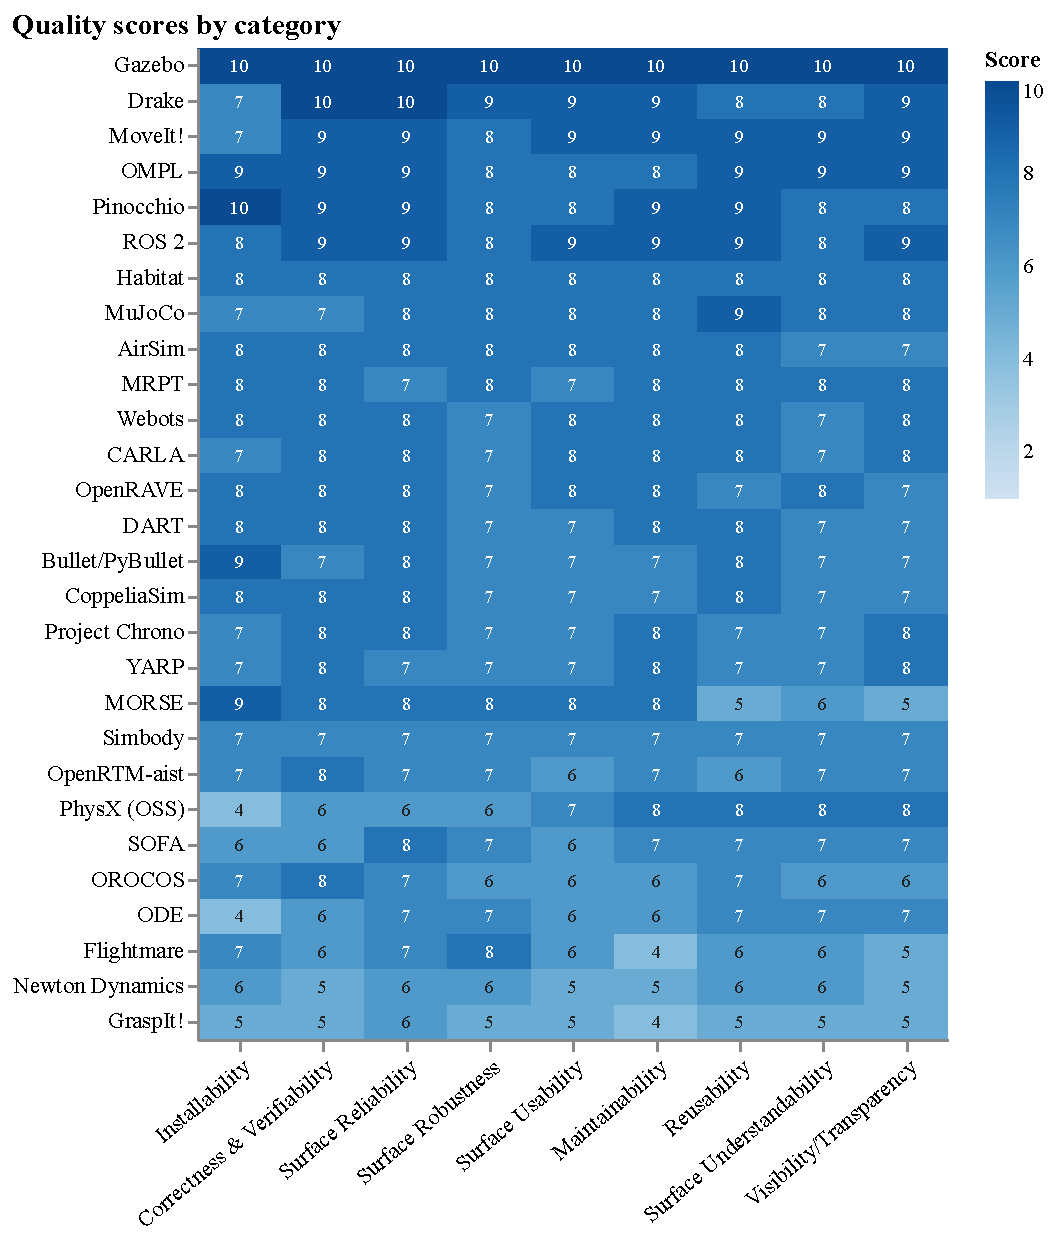
\includegraphics[width=0.95\textwidth]{figures/fig_quality_heatmap}
    \caption{Heatmap of the quality impression scores (1--10) for the 28 packages across the nine quality categories, ordered by unweighted mean.}
    \label{fig:quality-heatmap}
\end{figure}

\begin{figure}[htbp]
    \centering
    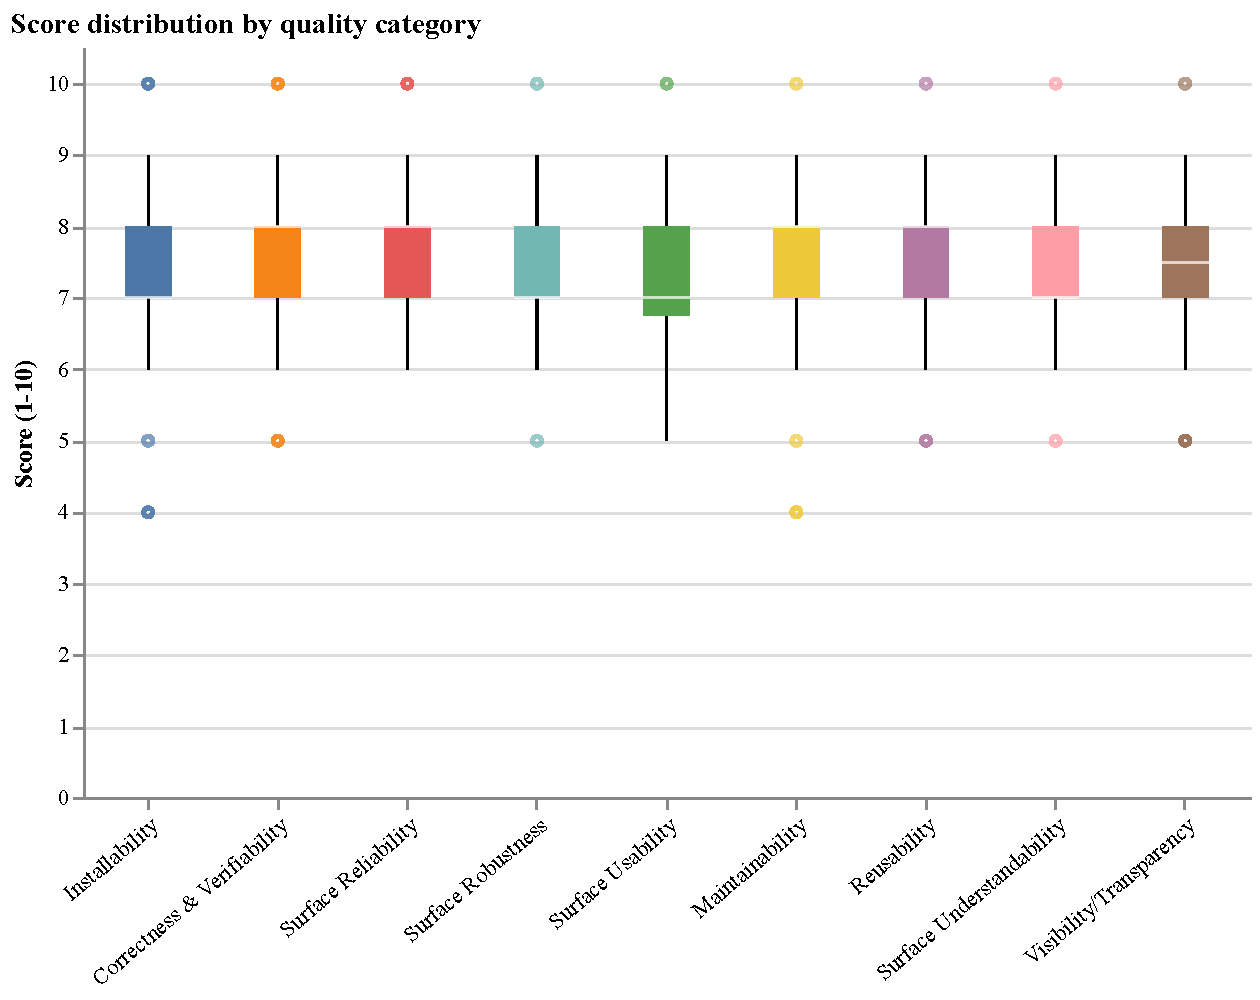
\includegraphics[width=0.95\textwidth]{figures/fig_category_distribution}
    \caption{Distribution of the impression scores across the 28 packages within each of the nine quality categories (box plots).}
    \label{fig:category-distribution}
\end{figure}

A handful of packages anchor the top of the table. Gazebo scores 10 in all nine categories, the only such sweep in the study. Within this template and time budget, no measured indicator separated it from the top of each scale; this is not a claim that the software is flawless. Drake and MoveIt! score 9 or 10 across most categories, and ROS~2, OMPL, and Pinocchio sit just below them. These packages share several traits: established stewardship (large organizations or active research groups), continuous contributor activity, comprehensive documentation, automated testing wired into CI/CD, and published contribution guidelines and release notes. None of these traits is individually decisive, but the combination separates the top tier from the rest.

For comparability with the descriptive summaries reported in the LBM and Medical Imaging assessments~\citep{Smith2024LBM,Smith2024MI}, Table~\ref{tab:overall-impressions} was also examined using a top-two coverage rule. A package was counted when it occupied one of the two highest distinct impression-score tiers in at least two of the nine quality categories. Six of the 28 packages (21\%) meet this criterion: Gazebo, Drake, MoveIt!, OMPL, Pinocchio, and ROS~2. The corresponding studies reported 67\% for LBM and almost 70\% for Medical Imaging. This difference does not establish that the MPS domain is unhealthy: the statistic is sensitive to tied scores, score calibration, the qualities measured, and the package-selection process in each study. Here it is used only to characterize the concentration of top-tier performance, which is clustered in a small leading group rather than broadly distributed across the sample.

\begin{figure}[htbp]
    \centering
    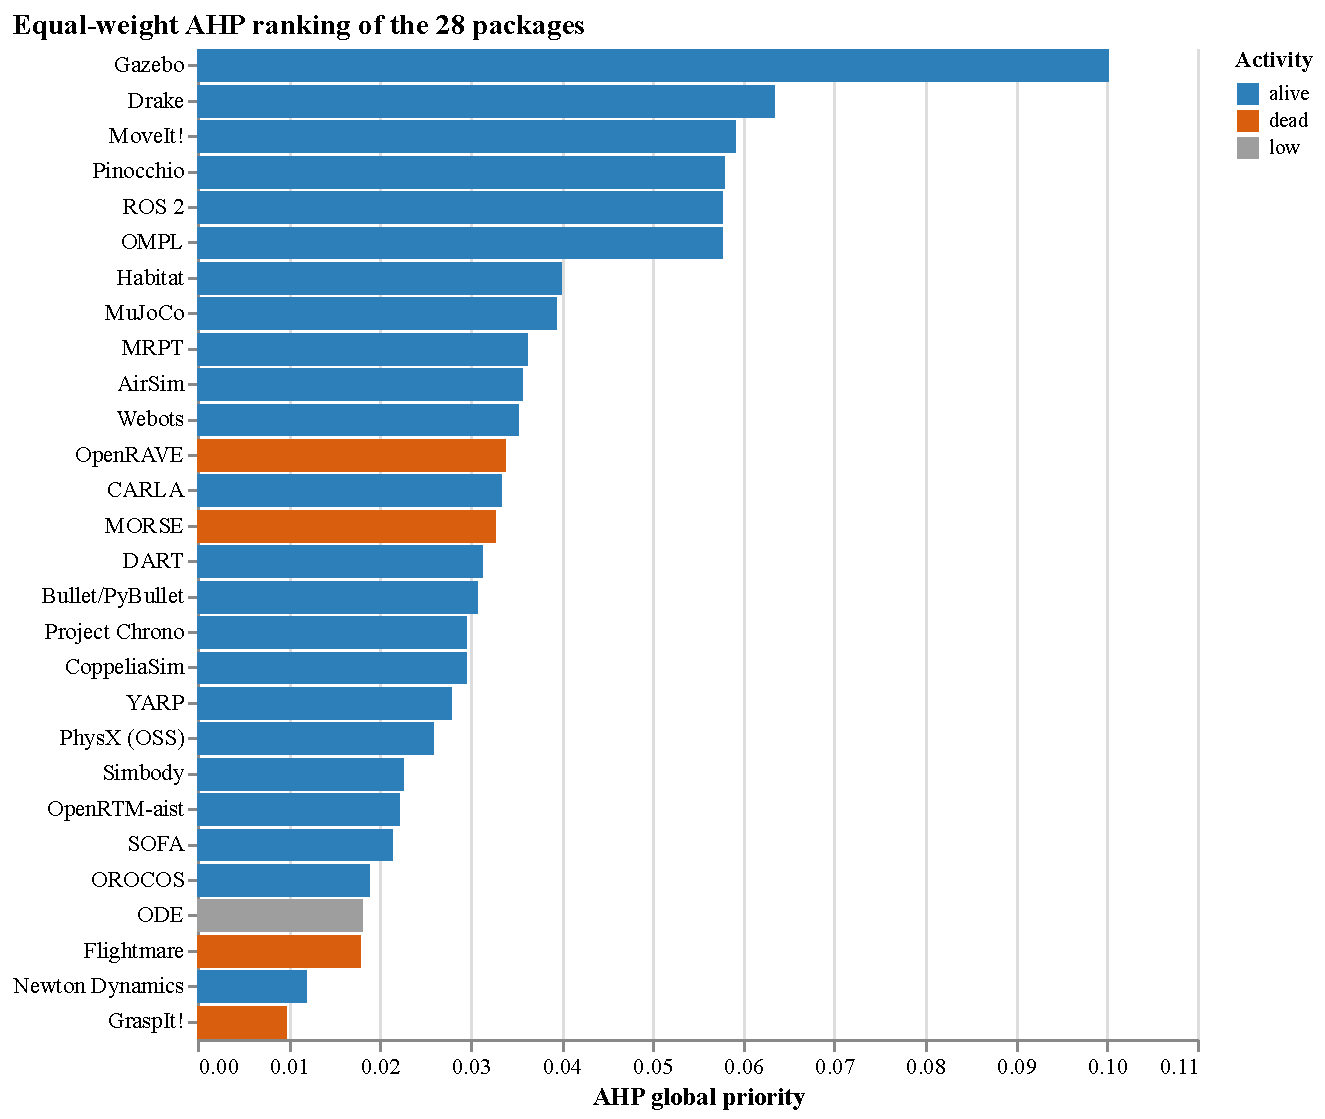
\includegraphics[width=0.92\textwidth]{figures/fig_ahp_ranking}
    \caption{Equal-weight AHP global-priority ranking ($c_k = 1/9$) of the 28 packages.}
    \label{fig:ahp-ranking}
\end{figure}

The AHP and arithmetic-mean orderings are close but not identical. Across the 28 packages, their ranks have Spearman correlation $\rho=0.987$ and Kendall correlation $\tau=0.944$. Gazebo, Drake, and MoveIt! occupy the same first three positions. The largest change is MORSE, which moves from 19th by arithmetic mean to 14th by AHP; all other packages move by at most three positions. AHP first converts each quality's pairwise score differences into a local priority vector and then aggregates those vectors. Equal criterion weights therefore do not reduce the calculation to an arithmetic mean of the original 1--10 scores.

To check that this ordering does not hinge on the precise impression scores, the AHP ranking was recomputed under a Monte~Carlo perturbation of its inputs. Each of the 252 score entries in Table~\ref{tab:overall-impressions} was independently scaled by a factor drawn uniformly from $[0.9, 1.1]$ (a $\pm 10\%$ perturbation clipped to the 1--10 range), and the equal-weight global priorities were re-derived over $1{,}000$ trials with a fixed random seed.

The ordering is well preserved: the mean Spearman rank correlation with the baseline is $0.97$ (minimum $0.87$) and the mean Kendall~$\tau$ is $0.88$ (minimum $0.74$). Gazebo remains top-ranked in every trial, and the two lowest, Newton~Dynamics and GraspIt!, are likewise fixed. The five highest-scoring packages after Gazebo never leave the top eight positions, though they are interchangeable within that band, with Drake alone ranging over ranks 2--6 (Figure~\ref{fig:ahp-sensitivity}).

The exact ordering among the leaders should therefore not be over-interpreted: the precise top-three and top-five sets recur in only $22\%$ and $26\%$ of trials, because their score gaps are smaller than the perturbation. The largest movement, up to ten positions, occurs in the densely packed middle of the table. The check thus supports the coarse structure of the ranking: a clear leader, a stable leading tier, a closely packed middle, and a fixed bottom (Section~\ref{sec:ahp-background}).

\begin{figure}[htbp]
    \centering
    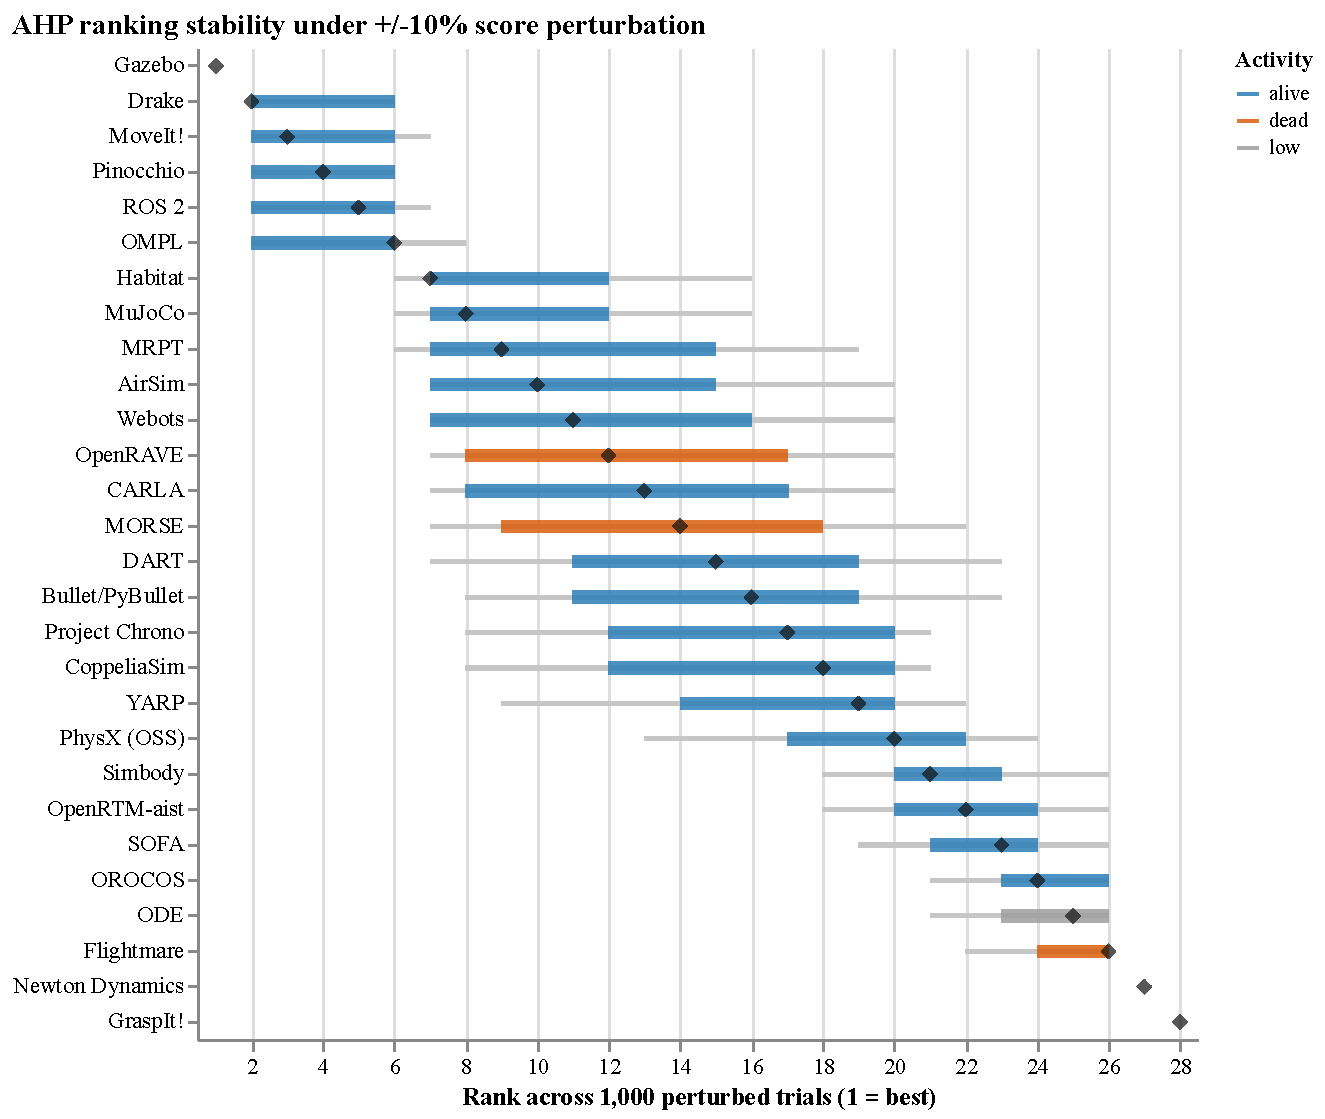
\includegraphics[width=0.92\textwidth]{figures/fig_ahp_sensitivity}
    \caption{Stability of the equal-weight AHP ranking under a $\pm 10\%$ score perturbation. Diamond, baseline rank; thick bar, 5th--95th percentile; thin line, full range.}
    \label{fig:ahp-sensitivity}
\end{figure}

The bottom of the table tracks maintenance status, but only loosely. GraspIt!, Flightmare, and MORSE (the dead packages of Section~\ref{sec:repository-project-metadata}) appear in the lower tier for most quality categories. Newton Dynamics, though technically alive at the May 2026 measurement date, joins them, reflecting its largely individual-maintained codebase and thin documentation infrastructure. OpenRAVE is also classified as dead under the 18-month rule, but its quality scores cluster in the middle of the table rather than the bottom; the documentation, test infrastructure, and codebase organization built during years of active development have not visibly degraded. In short, packages that go inactive tend to accumulate outdated documentation, broken installation procedures, and unresolved issues, but the rate at which they do so depends on the engineering capital accumulated before they went quiet.

Installability is generally strong across the MPS domain, most plausibly because of the widespread adoption of standard package managers (APT, pip, Conda), containerization (Docker), and CMake-based builds in the robotics community.

Documentation is universally present but varies in depth. All packages provide tutorials, user manuals, and API documentation, but the two indicators that record explicit engineering intent, coding standards and documented user characteristics, are far less common. The same gaps appear in the medical imaging and LBM samples~\citep{Smith2024MI,Smith2024LBM}, so they look more like patterns of research software practice than peculiarities of MPS. Figure~\ref{fig:key-indicators} summarizes this contrast across the template: the indicators tied to day-to-day installation and use sit at or near full coverage, while coding standards and documented user characteristics fall to 50\% and 4\%.

\begin{figure}[htbp]
    \centering
    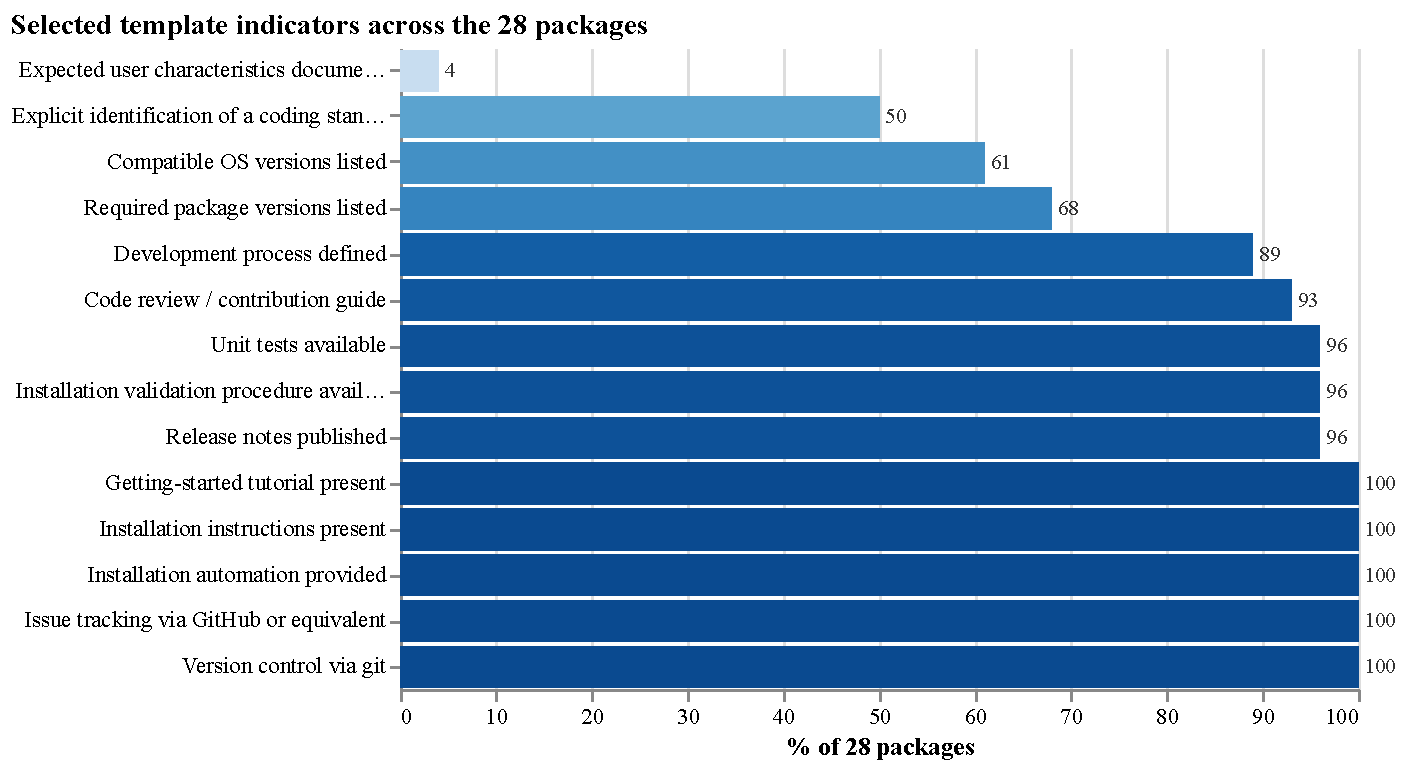
\includegraphics[width=0.92\textwidth]{figures/fig_key_indicators}
    \caption{Coverage of selected measurement-template indicators across the 28 packages, sorted from least to most common.}
    \label{fig:key-indicators}
\end{figure}

Repository activity is concentrated in a small subset of packages, with a few large or long-running projects accounting for a disproportionate share of total commits while several others show minimal activity in the last 12 months (Section~\ref{sec:repository-metrics-results}).
\section{Comparison with Community Indicators}
\label{sec:quality-vs-community}

The AHP priority (Section~\ref{sec:overall-observations}) combines the nine measured quality scores, while repository stars capture attention accumulated by a particular GitHub repository. Table~\ref{tab:quality-vs-community} compares these two rankings; ODE is omitted from the star ranking because its Bitbucket watcher count is not the same measure.

\begin{table}[p]
\centering
\caption{Equal-weight AHP rank versus GitHub stars rank. $\Delta = S - A$: positive values indicate a higher AHP rank than stars rank; negative values indicate a higher stars rank. Ties receive the same rank. ODE is excluded from the stars rank because its host reports watchers rather than GitHub stars (Table~\ref{tab:repository-metrics}).}
\label{tab:quality-vs-community}
\small
\singlespacing
\begin{tabular}{@{}P{2.5cm}rcrrr@{}}
\toprule
\textbf{Software} & \textbf{AHP Priority} & \textbf{A-Rank} & \textbf{Stars} & \textbf{S-Rank} & \textbf{$\Delta$} \\
\midrule
Gazebo          & 0.10012 & 1  & 1,337  & 17 & $+16$ \\
Drake           & 0.06339 & 2  & 4,025  & 8  & $+6$  \\
MoveIt!         & 0.05909 & 3  & 1,803  & 15 & $+12$ \\
Pinocchio       & 0.05795 & 4  & 3,354  & 10 & $+6$  \\
ROS~2           & 0.05775 & 5  & 5,475  & 5  & $0$   \\
OMPL            & 0.05765 & 6  & 2,047  & 14 & $+8$  \\
Habitat         & 0.03994 & 7  & 3,662  & 9  & $+2$  \\
MuJoCo          & 0.03939 & 8  & 13,440 & 4  & $-4$  \\
MRPT            & 0.03621 & 9  & 2,133  & 13 & $+4$  \\
AirSim          & 0.03571 & 10 & 18,159 & 1  & $-9$  \\
Webots          & 0.03527 & 11 & 4,345  & 7  & $-4$  \\
OpenRAVE        & 0.03387 & 12 & 801    & 21 & $+9$  \\
CARLA           & 0.03336 & 13 & 13,941 & 3  & $-10$ \\
MORSE           & 0.03276 & 14 & 367    & 23 & $+9$  \\
DART            & 0.03128 & 15 & 1,081  & 19 & $+4$  \\
Bullet/\allowbreak{}PyBullet & 0.03078 & 16 & 14,465 & 2 & $-14$ \\
Project Chrono  & 0.02953 & 17 & 2,836  & 11 & $-6$  \\
CoppeliaSim     & 0.02953 & 17 & 146    & 25 & $+8$  \\
YARP            & 0.02785 & 19 & 590    & 22 & $+3$  \\
PhysX (OSS)     & 0.02586 & 20 & 4,532  & 6  & $-14$ \\
Simbody         & 0.02257 & 21 & 2,521  & 12 & $-9$  \\
OpenRTM-aist    & 0.02216 & 22 & 24     & 26 & $+4$  \\
SOFA            & 0.02138 & 23 & 1,194  & 18 & $-5$  \\
OROCOS          & 0.01893 & 24 & 879    & 20 & $-4$  \\
ODE             & 0.01810 & 25 & ---    & ---& ---   \\
Flightmare      & 0.01793 & 26 & 1,353  & 16 & $-10$ \\
Newton Dynamics& 0.01195 & 27 & 24     & 26 & $-1$  \\
GraspIt!        & 0.00971 & 28 & 213    & 24 & $-4$  \\
\bottomrule
\end{tabular}
\end{table}

The 28 packages fall into four broad patterns in Table~\ref{tab:quality-vs-community}.

\textbf{Rough agreement at the top.} ROS~2 has rank 5 on both indicators. Drake ($\Delta=+6$), Pinocchio ($+6$), and Habitat ($+2$) also sit near the top of both lists.

\textbf{High AHP priority, lower repository visibility.} Gazebo ($\Delta=+16$), MoveIt! ($+12$), and OMPL ($+8$) are near the top of the AHP ranking but lower in stars. Gazebo's current repository omits attention accumulated before its repository reorganization; OMPL and MoveIt! are also used as dependencies inside larger workflows.

\textbf{High repository visibility, mid-pack AHP priority.} Bullet/PyBullet and PhysX (both $\Delta=-14$), CARLA ($-10$), and AirSim ($-9$) sit near the top in stars but in the middle or lower half of the AHP ranking. Their audiences extend into gaming, autonomous-driving research, and real-time physics, so repository attention need not track the research-software practices measured here.

\textbf{Low on both indicators.} GraspIt! ($\Delta=-4$) and Newton Dynamics ($-1$) are near the bottom on both lists. Newton Dynamics is a repository-migration case (Section~\ref{sec:repository-project-metadata}); its original repository would place it higher in stars without changing its AHP result.

These patterns agree with the medical imaging study's finding that repository popularity and measurement-based rankings do not have a simple relationship~\citep{Smith2024MI}. The comparison is descriptive: stars are host-, age-, and migration-dependent, so Table~\ref{tab:quality-vs-community} does not test whether engineering practice causes popularity (Section~\ref{sec:threat-construct-validity}).

        \setcounter{figure}{0}
        \setcounter{equation}{0}
        \setcounter{table}{0}

  \chapter{Comparison with Other Research Software Domains}
\label{ch:comparison-research-software}

This chapter compares the findings for motion planning and simulation (MPS) software with prior State-of-the-Practice studies in other research software domains, especially Medical Imaging (MI) software~\citep{Dong2021} and Lattice Boltzmann Method (LBM) software~\citep{Smith2024LBM}. The goal is not to claim that one domain is better than another. The domains differ in age, user communities, computational goals, and measurement dates. Instead, the comparison identifies where MPS software follows patterns already observed in research software and where it appears to differ.

The comparison follows the structure used in the LBM study. That study compared LBM projects with other research software in terms of repository artifacts, tool usage, and development principles, processes, and methodologies~\citep{Smith2024LBM}. The same three dimensions map directly to RQ3, RQ4, and RQ5 in this report.

\section{Comparison of Repository Artifacts}
\label{sec:comparison-artifacts}

RQ3 asks how MPS projects compare to other research software domains with respect to the artifacts present in their repositories. In the LBM study, repository artifacts were grouped by frequency and compared with research software development guidelines~\citep{Smith2024LBM}. The same idea applies here: artifacts such as installation instructions, user manuals, API documentation, issue trackers, tests, release notes, and contribution guides make development activity visible and make software easier to install, inspect, reuse, and maintain.

Table~\ref{tab:mps-artifact-comparison-summary} summarizes the main artifact observations from Chapter~\ref{ch:measurement-results}. These counts are based on the May 2026 measurement snapshot.

\begin{table}[H]
\centering
\caption{Summary of selected artifacts and visible development evidence in MPS packages.}
\label{tab:mps-artifact-comparison-summary}
\begin{tabular}{@{}lrr@{}}
\toprule
\textbf{Artifact or evidence type} & \textbf{Packages} & \textbf{\%} \\
\midrule
Public source repository & 28/28 & 100\% \\
Installation instructions & 28/28 & 100\% \\
Installation automation & 28/28 & 100\% \\
Getting-started tutorial & 28/28 & 100\% \\
User manual & 28/28 & 100\% \\
API documentation & 28/28 & 100\% \\
Issue tracking & 28/28 & 100\% \\
Version control & 28/28 & 100\% \\
Unit tests visible or available & 27/28 & 96\% \\
Release notes & 27/28 & 96\% \\
Contribution or code-review guidance & 26/28 & 93\% \\
Explicit coding standard & 14/28 & 50\% \\
Documented expected user characteristics & 1/28 & 4\% \\
\bottomrule
\end{tabular}
\end{table}

The main artifact finding for MPS software is the near-universal presence of user-facing and developer-facing infrastructure. Every measured package provides installation instructions, some form of installation automation, a getting-started tutorial, a user manual, API documentation, issue tracking, and version control evidence. MPS compares well with prior State-of-the-Practice studies on this dimension. The MI study reported that 22 of 29 packages provided a user manual~\citep{Dong2021}, while all 28 MPS packages do so in the current measurement. The LBM study found that installation guides and tutorials were common artifacts but API documentation was rare in the measured LBM sample~\citep{Smith2024LBM}; in this study, every MPS package provides API documentation.

This difference likely reflects the way MPS software is used. Many MPS projects are not stand-alone research scripts; they are simulators, middleware systems, planning libraries, physics engines, or integration frameworks. Their users often need to install them into larger toolchains, call their APIs from other software, and combine them with robotics ecosystems such as ROS. That use pattern creates pressure for installation documentation, tutorials, and API references. The presence of these artifacts does not by itself prove high quality, but it does show that the MPS ecosystem has adopted many of the artifacts that make research software inspectable and reusable.

The comparison is less uniformly positive for formal software engineering artifacts. Only one MPS package documents expected user characteristics, and 14 of 28 explicitly identify a coding standard. The coding-standard result is stronger than in the MI and LBM comparison studies, but it still means that half of the measured MPS packages do not expose this artifact. The LBM study observed that research software projects often fall short of recommended artifacts such as roadmaps, coding standards, checklists, uninstall instructions, and formal design or requirements documentation~\citep{Smith2024LBM}. The MPS results follow the same broad pattern: practical artifacts that help users install, run, and call the software are widespread, while artifacts that record design intent, expected user assumptions, and explicit development rules are less common.

The MPS artifact profile therefore appears stronger than MI and LBM in several public-facing documentation categories, especially manuals and API documentation. Still, it does not eliminate the usual gap between research software practice and software engineering recommendations. MPS packages are generally well equipped for use and integration, but their repositories less often expose the rationale, process rules, and user assumptions behind that software.

\section{Comparison of Tool Usage}
\label{sec:comparison-tools}

RQ4 asks how MPS projects compare to other research software domains with respect to tool usage. In the LBM study, tool usage was discussed in terms of development tools, dependencies, and project management tools, with special attention to version control and continuous integration~\citep{Smith2024LBM}. The current measurement provides strong evidence for version control, issue tracking, build or installation automation, testing, API documentation, and visible development infrastructure. Evidence for documentation-generation tools is narrower, since these tools are recorded for 12 of 28 packages.

Version control and issue tracking provide the most direct tool comparison. All 28 MPS packages use git-based version control and host public repositories on GitHub or an equivalent public platform. All 28 packages also use GitHub Issues or an equivalent issue tracker. The LBM study reported version control for 67\% of all LBM packages and 73\% of alive LBM packages~\citep{Smith2024LBM}. The MPS result is higher, although part of that difference comes from the current study design: repository-based measurement requires public repository evidence, so packages without suitable public repositories are filtered out before measurement. Even with that caveat, the result shows that the measured MPS ecosystem is strongly aligned with contemporary repository-centered development.

Build and installation automation are also widespread in the MPS sample. All 28 packages provide some form of installation automation, such as build files, scripts, package-manager support, or container-based installation support. This matters because MPS packages often depend on compiled C++ code, Python bindings, physics libraries, graphics systems, middleware, and operating-system packages. Manual installation would make such systems difficult to reproduce. The strong installability result in Chapter~\ref{ch:measurement-results} suggests that MPS maintainers have invested in build and installation tooling to reduce this burden.

Testing and verification tooling are also visible. Unit tests are available for 27 of 28 packages, automated testing is recorded for 26 packages, assertions are recorded for 23 packages, and documentation-generation tools are recorded for 12 packages. This matters for the LBM comparison because the LBM study treated test cases as an uncommon artifact and discussed automated testing as one of the prerequisites for effective continuous integration~\citep{Smith2024LBM}. In the MPS sample, testing evidence is much more common. This does not mean that every package has complete test coverage, nor that the tests exercise realistic robotics workloads. It does show, however, that test infrastructure is a visible part of most measured MPS projects.

Continuous integration should be interpreted more cautiously. Chapter~\ref{ch:measurement-results} records whether packages have a defined development process, often visible through CI/CD workflows, contribution guides, pull request templates, or issue templates. Twenty-five of 28 packages have such visible development-process evidence. This does not mean that 25 packages all use continuous integration in the same way or to the same depth. Some may use CI for builds, others for tests, documentation, static checks, packaging, or release automation. The narrower conclusion is that MPS repositories often expose automation and workflow infrastructure, but this report does not treat CI maturity as a separately ranked measure.

API documentation is another point of difference. The MPS measurement found API documentation for all 28 packages. This should be separated from tool usage: documentation-generation tools such as Doxygen or Sphinx are explicitly recorded for 12 MPS packages, not for the full set. The LBM paper reported that roughly half of the LBM packages mentioned documentation-generation tools and that API documentation was rare~\citep{Smith2024LBM}. The MPS result is stronger on API documentation itself, likely because many MPS packages are libraries, frameworks, or middleware systems whose adoption depends on programmable interfaces.

Overall, MPS projects appear to use modern repository and development tools consistently in the categories visible from public repositories. The best-supported observations concern version control, issue tracking, installation automation, tests, and API documentation. Compared with MI and LBM, the clearest advantages are API documentation and testing evidence; basic repository infrastructure is at least comparable with MI and stronger than the LBM comparison point. The weaker point is not the absence of tools, but the uneven visibility of how tools are governed: coding standards, process rules, review expectations, and user assumptions are not documented as consistently as the tools themselves.

\section{Comparison of Principles, Processes, and Methodologies}
\label{sec:comparison-practices}

RQ5 asks how MPS projects compare to other research software domains with respect to principles, processes, and methodologies. This question is harder to answer from public artifacts alone because process is partly social. Repositories can show issue trackers, pull requests, release notes, contribution guides, and automated workflows, but they cannot fully reveal how teams make design decisions, how maintainers negotiate priorities, or how much informal review occurs outside the public repository.

Within that limitation, MPS projects show more visible process structure than many research software projects described in prior studies. Twenty-five of 28 MPS packages have evidence of a defined development process, typically through CI/CD workflows, contribution guides, pull request templates, issue templates, or similar repository artifacts. Twenty-seven of 28 publish release notes. Twenty-six of 28 provide contribution or code-review guidance. These artifacts indicate that many measured MPS projects expect external users or contributors and have created at least minimal structures for managing that interaction.

This contrasts with the LBM discussion of principles and process, where process evidence was often informal and was strengthened by interviews with developers~\citep{Smith2024LBM}. LBM developers described small-team practices, lead developer roles, informal peer review, and issue tracking. The current MPS study does not yet have approved interview findings, so it cannot make equivalent claims about internal team behaviour. What it can say is that public MPS repositories frequently expose the artifacts associated with open collaboration: issues, pull requests, contribution instructions, release records, and workflow files.

The MPS process picture is still incomplete in two ways. First, 14 of 28 packages explicitly identify a coding standard, so this artifact is more common in MPS than in the comparison studies but still absent from half of the sample. Second, only one package documents expected user characteristics. This limits traceability between the intended audience and the design of tutorials, APIs, examples, and support channels. These gaps echo the LBM paper's observation that research software often has practical documentation but weaker formal requirements and design rationale~\citep{Smith2024LBM}.

The heterogeneity of MPS software also affects process comparison. A full simulator such as Gazebo or Webots, a middleware platform such as ROS~2, and a planning library such as OMPL do not have identical development needs. Large ecosystem projects tend to expose more formal governance, release management, and contribution infrastructure. Smaller or older packages may provide source code and documentation but little explicit process description. For that reason, the comparison should not treat the 28 MPS packages as interchangeable products. The commonality analysis in Chapter~\ref{ch:selected-software-commonality} is important because it explains why different process expectations may be reasonable for different kinds of MPS software.

Taken together, the evidence suggests that MPS projects are relatively mature in visible, repository-based process infrastructure. They align with modern open-source practice through public issue tracking, version control, release notes, contribution guidance, and automation. They still resemble other research software domains in the weaker documentation of design rationale, user assumptions, coding standards, and formal process principles.

\section{Summary of Cross-Domain Findings}
\label{sec:cross-domain-summary}

The cross-domain comparison answers RQ3--RQ5 as follows.

For RQ3, MPS projects compare favourably with prior research software domains in the presence of repository artifacts. Installation instructions, installation automation, tutorials, user manuals, API documentation, issue tracking, version control, unit tests, release notes, and contribution guidance are common or near-universal in the measured MPS set. Compared with MI and LBM, the MPS sample appears especially strong in user manuals, API documentation, and testing evidence. Its basic repository infrastructure is comparable with MI and stronger than the LBM comparison point. The main gaps are formal artifacts: documented user characteristics, requirements-style information, design rationale, and explicit coding standards for the half of packages that do not record one.

For RQ4, MPS projects show strong tool adoption in the categories visible from public repositories. Version control and issue tracking are universal in the measured set, installation automation is universal, unit-test evidence is present in nearly all packages, and API documentation is present for every package. Read together, these numbers indicate that MPS software development is tightly connected to modern open-source tooling. The comparison should be read with care because the study filters for public, repository-measurable software; proprietary or closed-core robotics tools may follow different practices.

For RQ5, MPS projects show substantial public evidence of development processes, but the evidence is mostly artifact-based. Contribution guidance, release notes, issue tracking, and visible workflow infrastructure are common. More formal principles and process documentation are less consistent. This pattern places MPS software between two tendencies: it is more visibly tooled and documented than some prior research software domains, but it still shares the broader research software tendency to under-document design intent, requirements assumptions, and coding rules.

Taken as a whole, the measured MPS ecosystem shows a solid public-artifact profile. Its strengths are practical and integration-oriented: installability, tutorials, API documentation, version control, issue tracking, testing evidence, and release visibility. Its weaknesses are also familiar from prior research software studies: formal requirements, explicit user assumptions, coding standards, and design rationale remain less consistently documented. That mixed picture is the substance of this report's contribution: it characterizes the state of the practice in MPS software rather than recommending a single package as superior for all robotics tasks.

        \setcounter{figure}{0}
        \setcounter{equation}{0}
        \setcounter{table}{0}

  % Discussion folded into the body chapters per supervisor feedback;
  % research questions are answered throughout the report.
  %% Retired draft chapter.
%
% This file is intentionally not included from main.tex. Supervisor feedback folded
% the discussion material into the body chapters, recommendations, threats to
% validity, and conclusions. Do not re-enable this chapter without rewriting it
% against the current chapter structure; otherwise it will duplicate
% conclusion.tex and may revive stale interview wording.

  %      \setcounter{figure}{0}
  %      \setcounter{equation}{0}
  %      \setcounter{table}{0}

  \chapter{Developer Pain Points and Interview Findings}
\label{ch:developer-interviews}

This chapter is the result chapter for the developer interview component and addresses RQ6--RQ9. The interview protocol, recruitment logic, ethics status, and analysis procedure are described in Section~\ref{sec:interview-component} of Chapter~\ref{ch:methodology}; they are not repeated here. The purpose of this chapter is to report the developer pain points identified from the interviews, analyze the practices developers use or propose in response to those pain points, and relate the interview findings to the public-artifact evidence reported in Chapters~\ref{ch:selected-software-commonality} through~\ref{ch:comparison-research-software}.

The chapter is organized around the evidence base for the interviews, the recurring pain points reported by developers, the practices developers use to address those pain points, and the relationship between interview findings and repository-based measurements.

\section{Interview Evidence Base}
\label{sec:interview-evidence-base}

This section describes the evidence base for the interview findings. It reports the number of contacted projects, the number of participating developers, the number of represented MPS software packages, the form of the records used for analysis, and any limits imposed by consent or confidentiality.

\noindent\textit{[Interview evidence summary to be inserted: contacted projects, participating developers, represented packages, record type, and reporting constraints.]}

The interview evidence is distinct from the repository evidence used earlier in the report. Public artifacts show visible practices, such as documentation, issue tracking, releases, test evidence, and continuous-integration configuration. Interviews provide less visible information, such as internal decision making, perceived development obstacles, informal review practices, funding or time constraints, and the reasons behind particular engineering choices.

\section{Overview of Developer Pain Points}
\label{sec:developer-pain-points-overview}

This section answers RQ6 by summarizing the recurring pain points reported by MPS developers. The grouping is derived from the interview evidence rather than imposed only from prior studies. Prior State-of-the-Practice reports suggest useful comparison categories, such as resource constraints, testing and correctness, documentation, maintainability, tooling, and project management, but the final categories for the MPS domain reflect the interview responses.

\noindent\textit{[Pain-point summary table to be inserted: theme, number of participants or projects, supporting interview question or code, and brief interpretation.]}

If a developer reports a pain point that is specific to a single project or software role, the text identifies it as such rather than presenting it as a domain-wide finding.

\section{Practices Used to Address Pain Points}
\label{sec:practices-address-pain-points}

This section analyzes what developers report doing in response to the pain points identified in Section~\ref{sec:developer-pain-points-overview}. It separates practices that developers already use from practices they propose or are considering. That distinction is important because an implemented practice provides different evidence from a recommendation or aspiration.

\noindent\textit{[Practice-response analysis to be inserted: pain point, reported practice, status of the practice, and evidence of effect.]}

The analysis connects each practice to the pain point it addresses. For example, if developers discuss practices related to documentation, testing, continuous integration, release management, contribution review, modularization, or user support, the chapter states whether those practices were reported as current practice, past attempts, or future plans.

\section{Analysis by Software Quality}
\label{sec:interview-analysis-software-quality}

This section connects the interview findings to the software qualities measured in Chapter~\ref{ch:measurement-results}. The repository-based measurements cover installability, correctness and verifiability, surface reliability, surface robustness, surface usability, maintainability, reusability, surface understandability, and visibility and transparency. The interviews add developer explanations for why those qualities are difficult to improve or how teams try to improve them in practice.

\noindent\textit{[Quality-by-quality interview analysis to be inserted.]}

The analysis keeps developer-reported evidence separate from public-artifact evidence. For instance, an interview may reveal testing, review, release, or documentation practices that are not obvious from the repository. Conversely, a repository may expose artifacts that were not emphasized by the developer. The chapter uses these differences to refine the interpretation of the measurements, not to replace the measurement record.

\section{Comparison with Other Research Software Domains}
\label{sec:interview-cross-domain-comparison}

This section addresses RQ7 and RQ9 by comparing the MPS interview findings with findings from prior State-of-the-Practice studies, particularly the medical imaging and Lattice Boltzmann method reports discussed in Chapter~\ref{ch:comparison-research-software}. The comparison identifies pain points that appear across multiple domains and pain points that seem more specific to MPS software.

\noindent\textit{[Cross-domain comparison to be inserted: MPS pain point, similar MI/LBM finding, difference in context, and implication for future practice.]}

The comparison also supports future-practice recommendations. A practice observed in another research software domain is presented as a candidate practice for MPS only when the connection to an MPS pain point is clear. This avoids treating recommendations from other domains as automatically transferable.

\section{Summary of Interview Findings}
\label{sec:interview-summary}

This chapter closes by summarizing the evidence-based answers to RQ6--RQ9. The summary identifies the main MPS developer pain points, the practices developers use or propose to address them, how those pain points compare with other research software domains, and which future-practice recommendations are supported by the interview evidence.

\noindent\textit{[Summary of interview findings to be inserted: RQ6--RQ9 answers and recommendations supported by the interview evidence.]}

        \setcounter{figure}{0}
        \setcounter{equation}{0}
        \setcounter{table}{0}

  \chapter{Threats to Validity}
\label{ch:threats-to-validity}

This chapter discusses the main threats to the validity of the study. The threats arise from the candidate discovery process, the public-artifact measurement approach, the interpretation of quality scores, and the auxiliary data sources used.

\section{Candidate Discovery}
\label{sec:threat-candidate-discovery}

The candidate package set was assembled from academic survey papers, community-curated lists, and auxiliary LLM-assisted discovery. Source appearance counts reflect how often a package is cited across the collected sources, not the quality or fitness-for-purpose of the software. A package with high mention counts may simply have been available earlier or targeted at a broader audience than packages with fewer citations. Packages that were not referenced in any of the collected sources would not appear in the candidate set regardless of their technical merit.

\section{Measurement Consistency}
\label{sec:threat-measurement-consistency}

The quality measurements are based on evidence that was publicly available at the time of the study (May 2026). Scores reflect the state of the public repository and documentation at a single point in time; they may not reflect the current or historical state of a project. Different evaluators examining the same evidence may reach different conclusions on some quality questions. Where scoring required a judgement call, the rationale is recorded in the measurement template, but some subjectivity remains.

\section{Snapshot-Based Repository Data}
\label{sec:threat-snapshot-repository-data}

Repository metrics such as star counts, fork counts, open issues, commit frequency, and lines of code are snapshots recorded in May 2026. These metrics change continuously and should not be interpreted as stable measures of project health. A project with low activity at the time of measurement may have been more active in prior periods or may resume activity later.

\section{Use of LLM-Assisted Candidate Sources}
\label{sec:threat-llm-assisted-sources}

LLM-generated candidate lists were used as an auxiliary discovery source to supplement academic and community-curated sources. These lists may reflect the training data of the underlying model rather than an authoritative survey of the domain. They were treated as one input among several and were not used as the sole or primary basis for inclusion or exclusion decisions.

\section{Scope Boundaries}
\label{sec:threat-scope-boundaries}

The scope of this study is robotics software for motion planning and simulation. The boundary between in-scope and out-of-scope software requires judgement in some cases. Proprietary tools, discontinued projects, and narrowly scoped libraries were excluded based on criteria described in Chapter~\ref{ch:methodology}, but the boundary decisions affect which packages are measured and which comparisons are possible.

        \setcounter{figure}{0}
        \setcounter{equation}{0}
        \setcounter{table}{0}

  \chapter{Threats to Validity}
\label{ch:threats-to-validity}

Any study based on publicly available artifacts is constrained by what those artifacts can reveal. The threats below are organized by threat type: reliability, construct validity, internal validity, and external validity.

\section{Reliability}
\label{sec:threat-reliability}

All measurements are based on public evidence collected in May 2026 and reflect a snapshot of each repository at that moment (Section~\ref{sec:open-source-repository-measurement}); the same project measured earlier or later might score differently. Some quality questions also require judgement, such as whether documentation is adequate or project metadata complete enough to support a score, and these were performed by a single assessor without an independent inter-rater check. The rationale is recorded in the measurement template (Section~\ref{subsec:measurement-template}), but the impression scores summarize observations beyond the recorded checklist answers, so the recorded data alone cannot fully reconstruct them. The time budget of one to four hours per package bounds the depth of every check; the surface measures are shallow by design.

\section{Construct Validity}
\label{sec:threat-construct-validity}

The measurements use public artifacts as evidence for software qualities, a practical proxy that does not capture every aspect of the underlying constructs: visible testing evidence does not prove that a package is correct, and visible issue-tracking activity does not fully describe maintainability. Mention counts likewise measure how often a package appears across candidate sources, not how good the software is (Section~\ref{sec:mention-count-ranking}).

\section{Internal Validity}
\label{sec:threat-internal-validity}

The candidate set was built from academic survey papers, community-curated lists, and LLM-assisted discovery, with the LLM lists supplementing rather than driving the other two sources. Those lists reflect the training data of the model rather than an independent survey of the MPS domain, so a package unknown to the model could be absent from its output. The filtering decisions described in Section~\ref{sec:filtering-criteria} further shape the measured set, since a package can be excluded for being out of scope, closed source, inactive, or not measurable from public repositories.

\section{External Validity}
\label{sec:threat-external-validity}

The selected set covers open-source MPS software measurable through public artifacts. Proprietary platforms, discontinued projects, and narrowly scoped libraries may differ from the measured packages, so the results describe the selected open-source MPS sample, not all robotics software. Because the packages play different roles, comparisons are evidence about development practice across a domain rather than direct product-to-product comparisons.

The installation-based measurements were performed on a Linux virtual machine, so the installability, surface reliability, and surface robustness results reflect Linux behaviour only. The same packages may install and behave differently on Windows or macOS, and installation routes available at measurement time, such as distribution packages, may be absent on other operating systems or later distribution releases.

        \setcounter{figure}{0}
        \setcounter{equation}{0}
        \setcounter{table}{0}

  \chapter{Conclusions}
\label{ch:conclusions}

\section{Summary}
\label{sec:conclusion-summary}

This study assessed the state of the practice for robotics motion planning and
simulation (MPS) software by adapting the Domain~X methodology
(Chapter~\ref{ch:methodology}) to a new domain. From 295 consolidated candidate
names, 28 packages were selected and measured in May 2026 against the Domain~X
template, spanning full simulators, physics and dynamics engines, planning
libraries, manipulation frameworks, and middleware. A commonality analysis
(Chapter~\ref{ch:selected-software-commonality}) described the selected packages
as a software family, and the findings were compared with prior studies of the
state of the practice for medical imaging and Lattice Boltzmann method software.
A developer-interview component was designed and received MREB ethics clearance
(project~\#8215, 2026-06-22); recruitment is underway, but the interviews have
not yet been conducted, so their evidence is not reported here.

\section{Answers to Research Questions}
\label{sec:answers-research-questions}

\textbf{RQ1 (candidate packages).} Filtering the
295 candidates by open-source availability, repository-based measurability,
activity status, and scope coherence (Chapter~\ref{ch:methodology},
Appendix~\ref{appendix:full-candidate-software-list}) yielded the 28 measured packages; notable
exclusions include MATLAB/Simulink, Unity, NVIDIA Isaac Sim, and RaiSim (closed
core components), MRDS and USARSim (inactive), and GPMP2 and CHOMP
(single-algorithm scope).

\textbf{RQ2 (quality ranking).} Across the nine quality categories
(Chapter~\ref{ch:measurement-results}), the unweighted quality mean is led by
Gazebo (10.0), Drake (8.8), and a tied group of MoveIt!, OMPL, Pinocchio, and
ROS~2 (8.7); GraspIt! (5.0), Newton Dynamics (5.6), and Flightmare (6.1) rank
lowest, consistent with their inactive, migrated, or low-activity status. Category
means are tightly bunched (7.3--7.8), so the rankings separate the top and
bottom tiers more clearly than the middle. An elicited-weight AHP ranking remains future work; an illustrative
equal-weight AHP ranking reproduces the same leaders.

\textbf{RQ3 (repository artifacts).} Practical artifacts are near-universal in the MPS sample
(Chapter~\ref{ch:comparison-research-software}):
installation instructions, installation automation, tutorials, user manuals,
API documentation, issue tracking, and version control are present for all 28
packages, which compares favourably with the medical imaging and LBM samples.
The recurring gaps are formal artifacts: documented user characteristics (1 of
28) and explicit coding standards (14 of 28).

\textbf{RQ4 (tool usage).} The measured MPS projects are tightly connected to
modern open-source tooling: git-based version control and issue tracking are
universal, continuous-integration evidence appears for 26 of 28 packages, and
documentation-generation tools are recorded for 12. The repository-based
inclusion rule partly explains this uniformity, but within the measured set tool
adoption is stronger than in the LBM comparison point and at least comparable
with medical imaging.

\textbf{RQ5 (principles, processes, and methodologies).} Process evidence is
visible but artifact-bound: 25 of 28 packages expose a defined development
process, 27 publish release notes, and 26 provide contribution guidance. What
repositories do not reveal---design rationale, requirements assumptions, and
internal decision making---remains under-documented in MPS software, the same
broad pattern reported for other research software domains.

\textbf{RQ6--RQ9 (pain points and practices).} These require
developer-interview evidence; Chapter~\ref{ch:developer-interviews}
records the planned evidence base, and
Chapter~\ref{ch:recommendations} gives artifact-based recommendations.
% TODO (after interviews): replace this paragraph with summarized answers to
% RQ6--RQ9 based on the approved interview records.

\section{Key Findings}
\label{sec:key-findings}

Four findings stand out from the artifact evidence. First, the practical
engineering infrastructure of MPS software is strong: every measured package
can be installed from documented instructions with some form of automation, and
only two installations broke during measurement, both recoverably. Second, the
weaknesses are concentrated in formal and explanatory artifacts rather than in
tooling: user assumptions, coding standards, and design rationale are the
recurring gaps. Third, community popularity and measured quality are different
signals: Gazebo leads on quality yet sits mid-table on stars,
and several highly starred packages place mid-table on quality,
so popularity indicators are not quality proxies. Fourth,
activity status only loosely predicts measured quality: packages that go
inactive decay at different rates depending on the engineering capital they
accumulated while active, as the contrast between OpenRAVE and GraspIt!
illustrates.

\section{Future Work}
\label{sec:future-work}

The most immediate direction is the developer-interview component: completing
recruitment, the interviews, and the analysis would answer RQ6--RQ9 and connect the measured artifact gaps to the
pain points developers actually experience.
A second direction is an elicited-weight AHP ranking, replacing the equal weights
of Chapter~\ref{ch:measurement-results} with weights obtained by pairwise
comparison of the qualities. Longitudinal repeat measurements would track how the
domain's practices change over time, and the same methodology could be extended
to adjacent robotics software domains.

One further direction concerns the measurement process itself, since completing
the template by hand is the most time-consuming part of the work. An exploratory
trial in which an AI coding agent installed, verified, and measured two physics
engines (Appendix~\ref{appendix:ai-assisted-measurement}) produced factual
entries tied to public sources but subjective scores that still needed human
review. With a person checking the evidence, this kind of agent-assisted
measurement could make it practical to cover more packages, or to repeat the
measurements over time, without straining the time budget that constrains a
manual study.

        \setcounter{figure}{0}
        \setcounter{equation}{0}
        \setcounter{table}{0}

\begin{appendix}
    \chapter{Full Candidate Software List}
\label{appendix:full-candidate-software-list}

This appendix records the leading candidate software packages considered during candidate discovery (Section~\ref{sec:candidate-software-discovery}). Consolidating the names collected from academic survey papers, community-curated lists, and LLM-assisted discovery produced 295 unique candidates; the full ranked list is preserved in the supplementary project materials, and the counted sources are listed in Appendix~\ref{appendix:mention-count-source-list}. Table~\ref{tab:full-candidate-list} records every candidate that received at least four mentions, together with the explicitly excluded tools and a representative sample of lower-count candidates.

Each entry shows the candidate's primary role in the MPS workflow, its consolidated mention count, and its status after filtering. The status values are defined as follows. \textit{Measured}: selected for measurement and reported in Chapter~\ref{ch:measurement-results}. \textit{Excluded}: removed by an explicit, documented filtering decision (open-source availability, activity, or scope), with the rationale for each exclusion given in Appendix~\ref{appendix:excluded-software-packages}. \textit{Not selected}: remained in the candidate pool but was not chosen, because it fell below the mention-count cutoff, failed one of the filtering criteria of Section~\ref{sec:filtering-criteria}, or is subsumed by a measured package. In the Mentions column, ``w/~X'' means the candidate is counted within the consolidated entry of measured package X, and ``---'' means the candidate has no entry in the consolidated mention-count list and entered the candidate discussion through the scope and filtering review rather than through the counted sources.

\begin{singlespace}
\begin{longtable}{@{}p{3.7cm}p{4.6cm}cp{2.9cm}@{}}
\caption{Candidate software packages considered for measurement, with consolidated mention counts.}
\label{tab:full-candidate-list}\\
\toprule
\textbf{Package} & \textbf{Primary role} & \textbf{Mentions} & \textbf{Status} \\
\midrule
\endfirsthead
\toprule
\textbf{Package} & \textbf{Primary role} & \textbf{Mentions} & \textbf{Status} \\
\midrule
\endhead
AirSim & Simulator (autonomous vehicles) & 7 & Measured \\
Bullet/PyBullet & Physics engine & 16 & Measured \\
CARLA & Simulator (autonomous driving) & 6 & Measured \\
CoppeliaSim (V-REP) & Simulator (general robotics) & 13 & Measured \\
DART & Dynamics library & 6 & Measured \\
Drake & Toolbox (dynamics, planning, control) & 6 & Measured \\
Flightmare & Simulator (quadrotor) & 4 & Measured \\
Gazebo & Simulator (general robotics) & 22 & Measured \\
GraspIt! & Manipulation (grasping) & 4 & Measured \\
Habitat & Simulator (embodied AI) & 4 & Measured \\
MORSE & Simulator (academic robotics) & 6 & Measured \\
MoveIt! & Manipulation (motion planning) & 4 & Measured \\
MRPT & Library (mobile robotics) & 4 & Measured \\
MuJoCo & Physics engine & 12 & Measured \\
Newton Dynamics & Physics engine & 4 & Measured \\
ODE (Open Dynamics Engine) & Physics engine & 10 & Measured \\
OMPL & Motion planning library & 5 & Measured \\
OpenRAVE & Planning framework & 9 & Measured \\
OpenRTM-aist & Middleware (RT components) & 4 & Measured \\
OROCOS & Control framework & 5 & Measured \\
PhysX (open-source SDK) & Physics engine & 8 & Measured \\
Pinocchio & Dynamics library & 5 & Measured \\
Project Chrono & Multi-physics simulation & 4 & Measured \\
ROS~2 & Middleware and SDK & 10 & Measured \\
Simbody & Multibody dynamics library & 5 & Measured \\
SOFA & Simulation framework & 5 & Measured \\
Webots & Simulator (general robotics) & 16 & Measured \\
YARP & Middleware (humanoid robotics) & 4 & Measured \\
\midrule
NVIDIA Isaac Sim & Simulator (high-fidelity, AI) & 9 & Excluded (non-OSS) \\
Unity & Game engine / simulator & 8 & Excluded (non-OSS) \\
MATLAB / Simulink & Robotics development environment & 6 & Excluded (non-OSS) \\
RaiSim & Physics simulator & 4 & Excluded (non-OSS) \\
MRDS & Simulator (Microsoft) & 5 & Excluded (inactive) \\
USARSim & Simulator (robot/automation) & 5 & Excluded (inactive) \\
GPMP2 & Motion planning algorithm (reference impl.) & --- & Excluded (scope) \\
CHOMP & Motion planning algorithm (reference impl.) & 1 & Excluded (scope) \\
\midrule
Player / Stage & Middleware and 2D/3D simulation & 6 & Not selected \\
ROS (ROS~1) & Middleware (predecessor of ROS~2) & w/~ROS~2 & Not selected \\
iGibson / OmniGibson & Simulator (interactive household) & 3 & Not selected \\
ManiSkill & Simulator (manipulation benchmark) & 3 & Not selected \\
SAPIEN & Simulator (general robotics) & 3 & Not selected \\
RBDL & Rigid body dynamics library & 3 & Not selected \\
Crocoddyl & Optimal control library (DDP) & 3 & Not selected \\
RobotStudio & Industrial robot simulator (ABB) & 3 & Not selected \\
robosuite & Simulator (manipulation, MuJoCo-based) & w/~MuJoCo & Not selected \\
Orocos KDL & Kinematics and dynamics (component of OROCOS) & w/~OROCOS & Not selected \\
TrajOpt & Trajectory optimization library & 2 & Not selected \\
SBPL & Motion planning library (search-based) & 2 & Not selected \\
KineoWorks & Path planning (Siemens, commercial) & 2 & Not selected \\
Robotics Toolbox for MATLAB & Robotics toolbox (MATLAB) & 2 & Not selected \\
FCL & Collision and proximity queries & 2 & Not selected \\
Crazyswarm / Crazyswarm2 & Multi-drone control and planning & 2 & Not selected \\
CasADi & AD and nonlinear optimization & 2 & Not selected \\
RoboDK & Industrial robot simulator and OLP & 2 & Not selected \\
Tesseract & Planning environment (optimization) & 1 & Not selected \\
iDynTree & Multibody dynamics, estimation & 1 & Not selected \\
STOMP & Motion planning algorithm & 1 & Not selected \\
Navigation2 (Nav2) & Mobile robot navigation stack & 1 & Not selected \\
Polymetis & Robot controllers (PyTorch) & 1 & Not selected \\
acados & Real-time NMPC and MHE solvers & 1 & Not selected \\
do-mpc & Python MPC and MHE & 1 & Not selected \\
Delmia & Digital manufacturing suite (Dassault) & 1 & Not selected \\
ros2\_control & Robot control framework (ROS~2) & --- & Not selected \\
\bottomrule
\end{longtable}
\end{singlespace}

The 28 measured packages were selected after the mention-count ranking and the filtering criteria of Section~\ref{sec:filtering-criteria}. Among the not-selected entries, proprietary or industrial tools such as \textit{KineoWorks}, \textit{Robotics Toolbox for MATLAB}, \textit{RoboDK}, \textit{RobotStudio}, and \textit{Delmia} fall outside the open-source criterion; most others fell below the mention-count cutoff, and \textit{Player~/~Stage}, despite six mentions, no longer meets the 18-month activity criterion. \textit{ROS}~(ROS~1) is consolidated with ROS~2 in the mention counting; the active successor was measured so that the results reflect current practice.

        \setcounter{figure}{0}
        \setcounter{equation}{0}
        \setcounter{table}{0}

    \chapter{Mention Count Source List}
\label{appendix:mention-count-source-list}

This appendix lists the sources used to construct the consolidated mention-count ranking described in Section~\ref{sec:mention-count-ranking}. Sources fall into two categories: community-curated robotics software lists and academic survey or comparison papers. The auxiliary LLM-generated lists are not enumerated here; they are recorded as a single discovery source in the project materials (\texttt{examples/sofware-counting-webs.csv}) and are discussed in Section~\ref{subsec:llm-assisted-sources}.

\section*{Community-Curated Sources}

Table~\ref{tab:community-mention-sources} lists the 15 community-curated sources used for candidate discovery. Each source is a public list, GitHub Topic page, or Wikipedia article that aggregates robotics software relevant to motion planning or simulation.

\begin{table}[H]
\centering
\caption{Community-curated sources used for mention counting.}
\label{tab:community-mention-sources}
\small
\begin{tabular}{@{}p{4.6cm}p{8.2cm}@{}}
\toprule
\textbf{Source} & \textbf{Description} \\
\midrule
GitHub Topic: motion-planning & GitHub Topic page aggregating active motion planning projects. \\
GitHub Topic: robotics-simulation & GitHub Topic page aggregating robotics simulation projects. \\
GitHub Topic: path-planning & GitHub Topic page for path and motion planning. \\
GitHub Topic: robotics-navigation & GitHub Topic page for navigation and planning. \\
best-of-robot-simulators & Curated list of robotic simulators (knmcguire). \\
Awesome Robotics Libraries & Robotics library list with planning and simulation sections (jslee02). \\
Awesome Robotics (ahundt) & Comprehensive robotics list covering planning, optimization, and simulation. \\
Awesome Robotics (kiloreux) & Community-maintained robotics list with planning and simulation entries. \\
Awesome Motion Planning & Motion planning list covering classical and modern libraries (AGV-IIT-KGP). \\
Awesome Multibody Dynamics Simulation & Multibody dynamics and simulation list (jslee02). \\
Awesome Robotic Tooling & Robotic tools and libraries list (Ly0n). \\
Awesome ROS 2 & ROS~2 ecosystem list including navigation, planning, and simulation (fkromer). \\
Awesome Webots & Webots-focused ecosystem list (lukicdarkoo). \\
Awesome Robotics Projects & Robotics projects list with planning and simulation components (mjyc). \\
Wikipedia: Robotics simulator & Wikipedia article aggregating robotics simulator entries. \\
\bottomrule
\end{tabular}
\end{table}

\section*{Academic Sources}

Table~\ref{tab:academic-mention-sources} lists the academic sources used for candidate discovery. These papers compare or survey simulators and tools used in robotics research.

\begin{table}[H]
\centering
\caption{Academic sources used for mention counting.}
\label{tab:academic-mention-sources}
\small
\begin{tabular}{@{}p{6.8cm}p{6.0cm}@{}}
\toprule
\textbf{Source} & \textbf{Packages discussed} \\
\midrule
A Comparison of Humanoid Robot Simulators: A Quantitative Approach (arXiv:2008.04627) & Gazebo, Webots, V-REP/CoppeliaSim \\
A Study on the Challenges of Using Robotics Simulators for Testing (2020, arXiv:2004.07368) & Gazebo, Webots, MuJoCo, PyBullet \\
\bottomrule
\end{tabular}
\end{table}

The raw catalogue of these sources, including the URLs captured during discovery and the per-source package mentions, is preserved in \texttt{examples/sofware-counting-webs.csv}. The consolidated ranking with per-package mention counts is in \texttt{examples/software-list-counting-result.xlsx} (sheet \texttt{final.m}).

        \setcounter{figure}{0}
        \setcounter{equation}{0}
        \setcounter{table}{0}

    \chapter{Measurement Template}
\label{appendix:measurement-template}

This appendix reproduces the structure of the measurement template used in this report. The template is adapted from the Domain~X Appendix~B template~\citep{Smith2021} and is grouped into project metadata, the nine quality categories described in Section~\ref{sec:software-quality-attributes}, and repository metrics collected through the DomainX tooling. The full per-package responses are recorded in the project material \texttt{summary.csv}, with one row per question and one column per package. Each quality section ends with an overall impression score on a 1--10 scale.

\section*{Project Metadata}

\begin{itemize}
    \item Software name.
    \item URL.
    \item Affiliation: institution(s).
    \item Software purpose.
    \item Number of developers (commits-based count from repository logs).
    \item Funding source (unfunded, unclear, or funded with a string identifying the source).
    \item Initial release date.
    \item Last commit date.
    \item Status (alive, dead, or unclear; alive requires commits in the previous 18 months).
    \item License (GNU GPL, BSD, MIT, terms of use, trial, none, unclear, other).
    \item Supported platforms (Windows, Linux, macOS, Android, other).
    \item Software category (concept, public, or private).
    \item Development model (open source, freeware, commercial, or unclear).
    \item Number of publications mentioning the software.
    \item Source code URL.
    \item Programming languages.
    \item Whether performance was considered.
\end{itemize}

\section*{Installability}

\begin{itemize}
    \item Are installation instructions present?
    \item Are the instructions in one place (single document or web page)?
    \item Are the instructions linear (a single sequence of steps)?
    \item Are the instructions written assuming no dependencies are pre-installed?
    \item Are compatible operating system versions listed?
    \item Is the installation automated (makefile, script, installer, container)?
    \item If installation broke, was a descriptive error message displayed?
    \item Is there a specified way to validate the installation?
    \item Number of installation steps (including manual steps such as unzip).
    \item Operating system used for installation.
    \item Number of extra packages required before or during installation.
    \item Are required package versions listed?
    \item Are dependency installation instructions provided?
    \item Were there problems caused by uninstall (where applicable)?
    \item Overall installability impression (1--10).
\end{itemize}

\section*{Correctness and Verifiability}

\begin{itemize}
    \item Is there any reference to requirements specifications or theory manuals?
    \item What tools or techniques are used to build confidence in correctness (literate programming, automated testing, assertions, continuous integration, etc.)?
    \item Is there a getting-started tutorial?
    \item Are tutorial instructions linear?
    \item Does the tutorial provide an expected output?
    \item Does the tutorial output match the expected output?
    \item Are unit tests available?
    \item Is there evidence that performance was considered?
    \item Overall correctness and verifiability impression (1--10).
\end{itemize}

\section*{Surface Reliability}

\begin{itemize}
    \item Did the software break during installation?
    \item If installation broke, was a descriptive error message displayed?
    \item Did the software break during the initial tutorial test?
    \item If the tutorial test broke, was a descriptive error message displayed?
    \item If the tutorial test broke, was recovery possible?
    \item Overall surface reliability impression (1--10).
\end{itemize}

\section*{Surface Robustness}

\begin{itemize}
    \item Does the software handle unexpected or unanticipated input gracefully (data of the wrong type, malformed input, etc.)?
    \item For text input files, does the software handle modified line endings or other text-file edge cases?
    \item Overall surface robustness impression (1--10).
\end{itemize}

\section*{Surface Usability}

\begin{itemize}
    \item Is there a getting-started tutorial?
    \item Is there a user manual?
    \item Are expected user characteristics documented?
    \item What is the user support model (FAQ, user forum, email address for questions, etc.)?
    \item Overall surface usability impression (1--10).
\end{itemize}

\section*{Maintainability}

\begin{itemize}
    \item What is the current version number?
    \item Is there information on code review or contribution practices?
    \item Are non-code artifacts available, and which kinds?
    \item What issue tracking tool is in use?
    \item What percentage of identified issues are closed?
    \item What percentage of code consists of comments?
    \item Which version control system is in use?
    \item Overall maintainability impression (1--10).
\end{itemize}

\section*{Reusability}

\begin{itemize}
    \item How many code files are there?
    \item Is the API documented?
    \item Overall reusability impression (1--10).
\end{itemize}

\section*{Surface Understandability}

\begin{itemize}
    \item Is indentation and formatting style consistent?
    \item Is a coding standard explicitly identified?
    \item Are code identifiers consistent and meaningful?
    \item Are constants other than 0 and 1 hard-coded into the program?
    \item Are comments clear?
    \item Are parameters in the same order for all functions?
    \item Is the name or URL of any algorithm used mentioned?
    \item Is the code modularized?
    \item Overall surface understandability impression (1--10).
\end{itemize}

\section*{Visibility and Transparency}

\begin{itemize}
    \item Is the development process defined?
    \item Are there documents recording the development process and status?
    \item Is the development environment documented?
    \item Are release notes available?
    \item Overall visibility and transparency impression (1--10).
\end{itemize}

\section*{Repository Metrics}

Counts collected from the primary repository at the measurement date. For projects with multiple repositories, the choice of the primary repository is recorded as part of the measurement notes.

\begin{itemize}
    \item Number of text-based files.
    \item Number of binary files.
    \item Total lines in text-based files.
    \item Total lines added to text-based files.
    \item Total lines deleted from text-based files.
    \item Total number of commits.
    \item Commits per year for the last five years (or since project start if younger).
    \item Commits per month for the last twelve months.
    \item Code lines, comment lines, and blank lines in text-based files.
    \item Number of stars.
    \item Number of forks.
    \item Number of repository watchers.
    \item Number of open pull requests.
    \item Number of closed pull requests.
\end{itemize}

Each substantive question above corresponds to one row in \texttt{summary.csv}, with the per-package answer recorded in the column for that package. Including the supplementary entries (overall impression scores per category and the free-text additional-comments fields), the template contains approximately 108 fields per package.

        \setcounter{figure}{0}
        \setcounter{equation}{0}
        \setcounter{table}{0}

    \chapter{Excluded Software Packages}
\label{appendix:excluded-software-packages}

This appendix records software packages considered during candidate discovery but excluded before measurement, following the criteria in Section~\ref{sec:filtering-criteria}. A small number were also excluded to keep the selected set methodologically coherent.

\section*{Excluded for Lack of Open-Source Availability}

The packages in Table~\ref{tab:excluded-non-oss} have proprietary core components or closed source code, which prevents the repository-based measurement described in Section~\ref{sec:measurement-procedure}. Dr.~Giamou confirmed that excluding these tools on methodological grounds does not misrepresent the MPS domain.

\begin{table}[H]
\centering
\caption{Packages excluded for lack of open-source availability.}
\label{tab:excluded-non-oss}
\small
\begin{tabular}{@{}p{3.5cm}p{9.5cm}@{}}
\toprule
\textbf{Package} & \textbf{Reason for exclusion} \\
\midrule
MATLAB / Simulink & Proprietary software; source code not publicly available; development process not accessible through public repositories. \\
Unity & Game engine with robotics simulation capabilities, but the core simulation engine is proprietary. \\
NVIDIA Isaac Sim & Built on NVIDIA Omniverse; core platform components are not open source. \\
RaiSim & High-performance physics simulator; source code not publicly available under an open-source license. \\
\bottomrule
\end{tabular}
\end{table}

\section*{Excluded for Inactivity}

The packages in Table~\ref{tab:excluded-inactive} were excluded using the Domain~X 18-month repository-activity flag together with project-specific maintenance evidence (Section~\ref{subsec:activity-maintenance-status}): no commits or releases within the 18 months preceding the May 2026 measurement date, and no current maintenance.

\begin{table}[H]
\centering
\caption{Packages excluded on activity grounds.}
\label{tab:excluded-inactive}
\small
\begin{tabular}{@{}p{3.5cm}p{9.5cm}@{}}
\toprule
\textbf{Package} & \textbf{Reason for exclusion} \\
\midrule
MRDS (Microsoft Robotics Developer Studio) & No updates since 2012; no longer supported by Microsoft. \\
USARSim (Unified System for Automation and Robot Simulation) & No active maintenance; does not represent current practice. \\
\bottomrule
\end{tabular}
\end{table}

\section*{Excluded to Maintain Methodological Coherence}

The packages in Table~\ref{tab:excluded-scope} are public reference implementations of single motion planning algorithms rather than general-purpose simulators, planning frameworks, physics engines, or middleware. Comparing them alongside full stacks such as Gazebo, MoveIt!, or ROS~2 would distort both the commonality analysis and the cross-package measurements. They were excluded for methodological consistency, not on quality grounds.

\begin{table}[H]
\centering
\caption{Packages excluded to maintain methodological coherence.}
\label{tab:excluded-scope}
\small
\begin{tabular}{@{}p{3.5cm}p{9.5cm}@{}}
\toprule
\textbf{Package} & \textbf{Reason for exclusion} \\
\midrule
GPMP2 (Gaussian Process Motion Planner~2) & Single-algorithm optimization-based motion planning reference implementation; narrower in scope than the general-purpose packages that dominate the candidate list. \\
CHOMP (Covariant Hamiltonian Optimization for Motion Planning) & Single-algorithm optimization-based motion planning reference implementation; narrower in scope than the general-purpose packages that dominate the candidate list. \\
\bottomrule
\end{tabular}
\end{table}

The full filtered candidate list is preserved in the supplementary project materials; Appendix~\ref{appendix:full-candidate-software-list} records the leading candidates with their mention counts and dispositions.

        \setcounter{figure}{0}
        \setcounter{equation}{0}
        \setcounter{table}{0}

    \chapter{Interview Materials}
\label{appendix:interview-materials}

% Drafting note: this appendix reproduces the semi-structured interview guide
% referenced in Section~\ref{sec:interview-component}. Source: the MREB interview
% guide in the project materials (interview_materials/MACREM-2026). Include only
% approved ethics materials and interview artifacts that are actually available;
% do not invent interview data or findings.

This appendix reproduces the semi-structured interview guide referenced in Section~\ref{sec:interview-component}. The guide contains 18 questions in three groups: the interviewee's background, the development process and tools, and the software's users. The interviewer may adjust the exact wording during the conversation and may use short clarification prompts to ask for more detail or concrete examples.

\paragraph{Interviewee background.}
\begin{enumerate}
    \item What is your current position or title? What degrees do you hold?
    \item What is your contribution to, or relationship with, the software?
    \item How long have you been involved with this software?
\end{enumerate}

\paragraph{Developers, development process, tools, and techniques.}
\begin{enumerate}
    \setcounter{enumi}{3}
    \item How large is the development group?
    \item What is the typical background of a developer?
    \item Currently, what are the most significant pain points in your development process? Specifically, what are the pain points in requirements definition, design, implementation, and verification?
    \item How does documentation fit into your development process? Would improved documentation help with the obstacles you typically face?
    \item In the past, was there any major obstacle to your development process that has been solved? How did you solve it?
    \item What is your software development model? For example, waterfall, agile, or another model.
    \item What is your project management process? Are any project management tools used?
    \item Is it hard to ensure the correctness of the software? If there were obstacles, what methods have been considered or practiced to improve the situation? If practiced, did they work?
    \item When designing the software, did you consider the ease of future changes? For example, will it be hard to change the system structure, modules, or code blocks? What measures have been taken to support future changes and maintenance?
    \item Do you have any concern that your computational results will not be reproducible in the future? Have you taken any steps to ensure reproducibility?
    \item What positive contributions do LLM-based tools have on your development process with respect to documentation, coding, and testing?
    \item What negatives are associated with LLM-based tools?
\end{enumerate}

\paragraph{Users.}
\begin{enumerate}
    \setcounter{enumi}{15}
    \item What is the typical background of a user?
    \item Can you provide instances where users have misunderstood or misused the software? What actions, if any, were taken to address usability issues?
    \item Do you think the current documentation clearly conveys all necessary knowledge to users? If yes, how did you successfully achieve it? If no, what improvements are needed?
\end{enumerate}

        \setcounter{figure}{0}
        \setcounter{equation}{0}
        \setcounter{table}{0}

    \chapter{Exploratory AI-Assisted Measurement}
\label{appendix:ai-assisted-measurement}

This appendix records a small exploratory trial in which an AI coding agent
carried out this study's measurement protocol on its own, over two physics
engines from the selected set (PyBullet and MuJoCo), using the template of
Appendix~\ref{appendix:measurement-template} and the procedure of
Section~\ref{sec:measurement-procedure}. It is not part of the validated results
in Chapter~\ref{ch:measurement-results}; it is a feasibility check and the basis
for the future-work direction in Section~\ref{sec:future-work}. The agent worked
in a Linux shell with file-system and network access in early June 2026, so its
repository snapshots fall slightly later than the May 2026 snapshot of the main
study.

\section*{Task Given to the Agent}

The agent was given a single natural-language prompt and no installation commands;
it had to locate the official documentation, install each package, verify the
installation, and complete the template unaided. The prompt is reproduced below.

\begin{quote}
\small
Read the CSV file in the current directory and use the first column
(``Metric'') as the measurement template. Measure two software packages,
PyBullet and MuJoCo. The requirements were:
\begin{itemize}[noitemsep]
  \item Only fill in the columns for these two packages; do not modify the other
        software columns. A new CSV file may be created.
  \item Do not rely on user-provided installation commands; find the official
        documentation, GitHub README, or project website to determine the
        installation and verification steps.
  \item Follow each metric in the CSV to complete installation, verification,
        observation, and data entry.
  \item Take a screenshot at every step and save it to a screenshots folder.
        Screenshots must cover at least: reading the CSV, finding the official
        documentation, the installation steps, the verification steps, error
        messages or successful output, and the final CSV result.
  \item Evidence may come only from official documentation, GitHub, terminal
        output, and commands actually executed.
  \item Write ``unclear'' for uncertain values and ``n/a'' for values that do
        not apply.
  \item Also write a \texttt{notes.md} file recording the selected packages, the
        official links used, the commands run at each step, the screenshot
        filenames, whether installation succeeded, whether verification
        succeeded, which CSV cells were filled or changed, and any problems
        encountered with their recovery.
\end{itemize}
Complete Bullet/PyBullet first, then MuJoCo.
\end{quote}

\section*{Official Sources Located by the Agent}

The agent found the official sources in Table~\ref{tab:ai-pilot-sources} and used
them to choose the installation and verification steps.

\begin{table}[H]
\centering
\caption{Official sources the agent used for the two packages.}
\label{tab:ai-pilot-sources}
\small
\begin{tabular}{@{}p{2.6cm}p{3.8cm}p{6.2cm}@{}}
\toprule
\textbf{Package} & \textbf{Resource} & \textbf{Location} \\
\midrule
PyBullet & Website and forum  & \url{https://pybullet.org} \\
         & Source repository  & \url{https://github.com/bulletphysics/bullet3} \\
         & Python package     & \url{https://pypi.org/project/pybullet/} \\
\midrule
MuJoCo   & Website            & \url{https://mujoco.org} \\
         & Source repository  & \url{https://github.com/google-deepmind/mujoco} \\
         & Documentation      & \url{https://mujoco.readthedocs.io} \\
\bottomrule
\end{tabular}
\end{table}

\section*{Installation and Verification}

Both packages installed with a single \texttt{pip} command inside a Python
virtual environment, and both were verified with a short program that the agent
wrote and ran. Table~\ref{tab:ai-pilot-outcome} summarizes the outcome.

\begin{table}[H]
\centering
\caption{Installation and verification outcome of the AI-assisted trial.}
\label{tab:ai-pilot-outcome}
\small
\begin{tabular}{@{}p{3.1cm}p{4.7cm}p{4.7cm}@{}}
\toprule
\textbf{Item} & \textbf{PyBullet} & \textbf{MuJoCo} \\
\midrule
Install command     & \texttt{pip install pybullet} & \texttt{pip install mujoco} \\
Installed version   & 3.2.7 & 3.9.0 \\
Installation steps  & 1 (single pip command) & 1 (single pip command) \\
Extra packages      & none (self-contained) & bundled with the wheel \\
Operating system    & Linux (Ubuntu) & Linux (Ubuntu) \\
Verification        & Loaded the bundled \texttt{plane.urdf} model in DIRECT mode & Compiled an inline XML model of a free-jointed box on a plane \\
Result              & Succeeded & Succeeded \\
\bottomrule
\end{tabular}
\end{table}

The agent also queried the GitHub API and recorded the template's project
metadata, each entry tied to the source it read. For PyBullet
(\path{bulletphysics/bullet3}) it recorded 311 contributors, a zlib license, a
first commit in April 2011, and a most recent push in October 2025; for MuJoCo
(\path{google-deepmind/mujoco}), 116 contributors, an Apache-2.0 license, a
first commit in August 2021, and a most recent push in June 2026. These
contributor counts come from the GitHub contributors API, which returns fewer
entries than the commit-log method of the main study
(Section~\ref{subsec:repository-metrics}; 333 developers for Bullet/PyBullet,
138 for MuJoCo), so the two are not directly comparable.

\section*{Problems Encountered and Recovery}

The agent encountered three problems and recovered from each without manual
intervention. First, a direct \texttt{pip install} failed because the system
Python was externally managed; the agent created a virtual environment and
installed into it. Second, its first PyBullet verification script queried the
physics engine before connecting to it; the agent reordered the calls so the
connection came first. Third, no screenshot utility was present, so the agent
installed one.

\section*{Limitations and Relationship to the Main Study}

As a single run over two packages by one agent, this shows feasibility, not a
result. The checkable, factual entries (installation command, installed version,
license, contributor count, verification result) were each tied to a public
source and straightforward to confirm. The subjective impression scores and
free-text judgements were not validated here, and in places disagree with the
agent's own notes, which is the clearest reason a human must still review the
output before it can serve as evidence.

The trial's artifacts, the completed template and the notes document, are
preserved in the supplementary project materials. The trial motivates the
agent-assisted measurement under human supervision discussed in
Section~\ref{sec:future-work}.

        \setcounter{figure}{0}
        \setcounter{equation}{0}
        \setcounter{table}{0}
\end{appendix}

\bibliographystyle{plainnat}
\bibliography{references}

\label{NumDocumentPages}

\end{document}
% ********************************
